
\chapter{变率和微商}

从本章起,我们开始学习单变量的微积分学的基本概念和基础理论.

微积分学是研究变量的数学,变量之间的关系就是函数,因此,函数是微积分学研究的主要对象.

在函数的基本性质中,有两个最基本、最重要的概念-变率与求和,为了解决求函数的变率与求函数$f$在$[a,b]$上的和的问题就相应地产生微分与积分运算,而这两种运算之间,也存在着一种自然的互逆关系,在本章中,我们由函数的变率问题引出函数的微商(导数)概念,并给出初等函数的一套求导法则,在下一章中,我们揭示微分运算与积分运算的互逆关系,这就是微积分学的基本定理.

总起来说,微分反映了函数的局部性质,或在某个点附近的性质;积分则反映了函数的整体性质,或某个区间的性质;函数的局部性质与整体性质之间的有机联系,恰恰反映了微分运算与积分运算之间的互逆关系.

\section{微商(导数)的定义}
函数关系$y=f(x)$就是确定变量$y$如何随着变量$x$的变动而变动的关系,对于给定的函数$y=f(x)$, 变量$y$在变量$x$的不同点附近的变动情况是不尽相同的,这就是说,在变量$x$的
某个值$x_1$外,当$x_1$略加变动时,相应的$y$的变动可能相当剧烈(急增,或急减);而在变量$x$的另一个值$x_2$处,$y$的变动就可能较为迟缓,但是,用这样的语言来表达函数在某一点处的变率是不精确的,我们需要用“数量”来确切地表达这个意思,这就是函数在某点(或某时刻)的变率的问题,简称变率.

\subsection{直线函数的变率}
一次函数$f (x) =kx+b$
是一种最简单的函数,它的函数图象是一条斜率等于$k$的直线,如图2.1所示.
\begin{figure}[htp]
    \centering
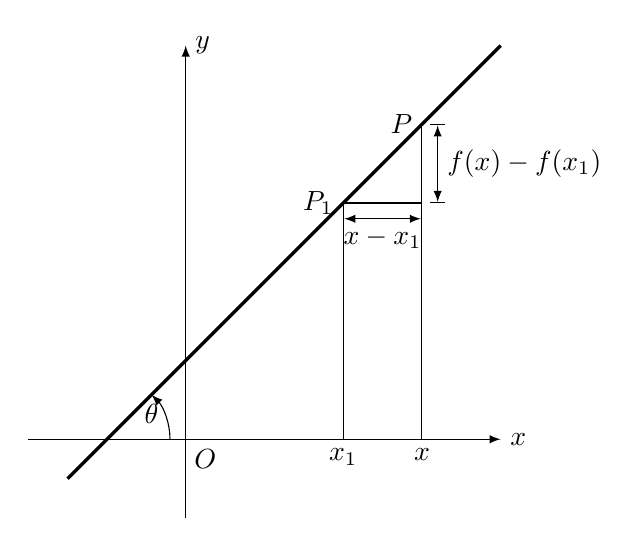
\begin{tikzpicture}[>=latex]
    \draw[->](-2,0)--(4,0)node[right]{$x$};
    \draw[->] (0,-1)--(0,5)node[right]{$y$};
    \draw[very thick] (-1.5,-.5)--(4,5);
\draw[->](-.2,0) arc (0:45:.8)node[below]{$\theta$};
\draw(2,3)node[left]{$P_1$}--(2,0)node[below]{$x_1$};
\draw(3,4)node[left]{$P$}--(3,0)node[below]{$x$};
\draw[|<->|](3.2,4)--node[right]{$f(x)-f(x_1)$}(3.2,3);
\draw[|<->|](2,2.8)--node[below]{$x-x_1$}(3,2.8);
\draw(2,3)--(3,3);\node at (.25,-.25){$O$};
\end{tikzpicture}
    \caption{}
\end{figure}

设$x_1$, $f(x_1)$和$x$, $f(x)$分别是直线上点$P_1$和$P$的坐标,为了反映函数变化快慢的问题,无论$x<x_1$还是$x>x_1$,自然地考虑在点$x_1$邻近,函数与自变量的相应的改变量的比:
\[\frac{f(x)-f(x_1)}{x-x_1}=\frac{(kx+b)-(kx_1+b)}{x-x_1}=k=\tan\theta\]
上面的表达式称为函数的\textbf{差商},它表示函数在区间$[x_1,x]$或$[x,x_1]$上对于自变量$x$的\textbf{平均变化率}.由于$k$是不随变量$x$变动而变动的常数,因此,一次函数在自变量的任何一个区间内的平均变化率都是常数.

如果让自变量的变化区间的长度无限地缩短,也就是让$x$无限地接近于$x_1$时,平均变化率所趋向的极限
\[\lim_{x\to x_1} \frac{f (x) -f (x_1)}{x-x_1} =k\]

\subsection{平滑曲线的切线与变率}
一般的函数$y=f(x)$的图象通常不是直线,由于函数
和它的图象的多样性,为了讨论的方便起见,我们先把讨论的范围限制在“平滑”的曲线上,常用的函数$y=f(x)$的图象往往是“平滑的”,平滑性的直观内涵是:用愈高倍的显微镜去观察曲线的微段,就愈象直线段,比较明确的几何说法是:一条曲线在$P$点的平滑性就是存在唯一的一条过$P$点的切线,它无限地逼近曲线在$P$点邻近的微段,于是,当$y=f(x)$的图象$C$在$P$点存在唯一的一条切线时,我们就说曲线$C$在$P$点平滑,而$P$点叫做曲线的平滑点,一条在每点都平滑的曲线叫做平滑的曲线,一个函数的图象平滑曲线时,我们就称这种函数为平滑函数.

同学可能会问这样一个问题:在曲线的点$P$存在唯一的一条切线的含义是什么?因为迄今我们对于一般的曲线的切
线还未下过定义呢!

我们从图2.2和2.3注意到不能把切线定义为与曲线只有一个交点的直线.这样的定义限制得既太紧同时又太松.因
为,照此定义,图2.2所示的直线就不是过曲线上$P$点的切线了,实际上,尽管图2.2的直线与曲线还有一个交点$Q$, 但它在曲
线$P$点邻近却与曲线密合,故仍应该是过曲线$P$点的切线;又图2.3表明过抛物线上任何一点$P$与$y$轴平行的直线虽然与抛物线只有一个交点,但它的其余部分却远离$P$点邻近的弧,故它不应该是抛物线的切线,定义切线的可行途径是从割线开始,并应用极限的概念.

\begin{figure}[htp]
    \centering
    \begin{minipage}[t]{0.48\textwidth}
    \centering
    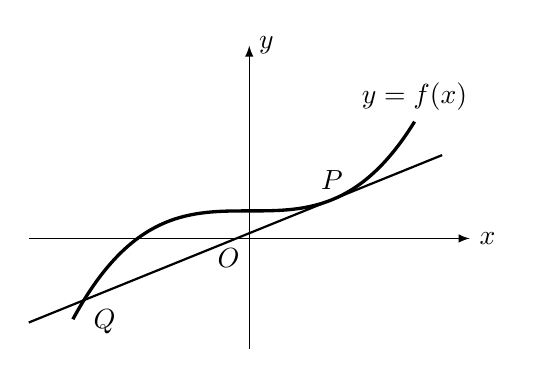
\begin{tikzpicture}[>=latex, scale=.7]
\draw[->](-4,0)--(4,0)node[right]{$x$};
\draw[->](0,-2)--(0,3.5)node[right]{$y$};
\draw[domain=-3.2:3, very thick, samples=100]plot(\x, {.06*\x^3+.5})node[above]{$y=f(x)$};
\node at (0,0)[below left]{$O$};
\node at (1.5,.7025)[above]{$P$};
\draw[domain=-4:3.5, samples=10, thick]plot(\x, {.405*\x+.095});
\node at (-3,-1.12)[below right]{$Q$};
    \end{tikzpicture}
    \caption{}
    \end{minipage}
    \begin{minipage}[t]{0.48\textwidth}
    \centering
    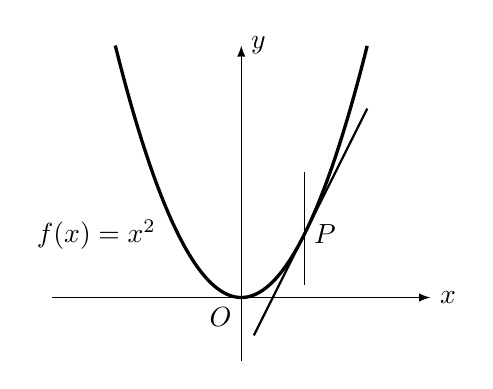
\begin{tikzpicture}[>=latex, scale=.8]
  \draw[->](-3,0)--(3,0)node[right]{$x$};
\draw[->](0,-1)--(0,4)node[right]{$y$};
\draw[domain=-2:2, very thick, samples=100]plot(\x, {\x*\x});
\node at (-1.2,1)[left] {$f(x)=x^2$};
\draw(1,0.2)--(1,2);
\node at (1,1)[right]{$P$};
\node at (0,0)[below left]{$O$};
\draw[domain=.2:2, samples=10, thick]plot(\x, {2*\x-1});


    \end{tikzpicture}
    \caption{}
    \end{minipage}
  \end{figure}



如图\ref{fig:PQ_tangent}所示,取曲线$y=f(x)$上点$P$附近的另一点$Q$, 通过这两点画一条直线,这直线叫做过曲线上$P$点的割线,让$Q$点沿曲线向点$P$移动,这条割线将达到极限位置,此极限位置与$Q$点从哪一侧趋向于$P$是无关的,我们称这个割线的极限位置为过曲线上$P$点的切线.

\begin{figure}[htp]
    \centering
\begin{tikzpicture}[>=latex, scale=1.5]
    \draw[->](-.5,0)--(4,0)node[right]{$x$};
    \draw[->](0,-.5)--(0,3)node[right]{$y$};
    \node at (0,0)[below left]{$O$};
    \draw[domain=.5:3.2, samples=100, very thick]plot(\x, {-.5*(\x-2.25)^2+2})node[right]{$y=f(x)$};
    \tkzDefPoints{1/1.22/P, 3/1.72/Q, 3.5/1.22/P'}
    \tkzLabelPoints[above](P,Q)
    \tkzDrawSegments(P,P')
    \draw[domain=.2:2, samples=10, thick]plot(\x, {1.25*\x-0.03});
    \tkzDefPoints{3/3.72/Q'}
    \tkzDrawLines(P,Q)
    \tkzMarkAngles[mark=none, size=.7](P',P,Q)
    \tkzMarkAngles[mark=none, size=.3](P',P,Q')
    \tkzLabelAngle[pos=.5](P',P,Q'){$\alpha_1$}
    \tkzLabelAngle[pos=.9](P',P,Q){$\alpha$}
\end{tikzpicture}
    \caption{}\label{fig:PQ_tangent}
\end{figure}

割线的这种极限位置的存在性这一假设,与曲线在点$P$具有唯一的一条切线或确定的方向的假设是等价的.

现在我们要对曲线$y=f(x)$用解析式子把割线的这种极限位置存在的过程表示出来.
设$\alpha$是割线$PQ$同正$x$轴构成的夹角,$\alpha_1$是过点$P$点的切线同正$x$轴构成的夹角,于是
\[\lim_{Q\to P}\alpha=\alpha_1\]
设$x_1,y_1$和$x,y$分别是点$P$和$Q$的坐标,这时,我们立即得到
\[\tan\alpha=\frac{y-y_1}{x-x_1}=\frac{f(x)-f(x_1)}{x-x_1}\]
因此,上述求极限的过程(不考虑垂直切线$\alpha_1=\frac{\pi}{2}$的情况)可由下式来表示:
\[\lim_{x\to x_1}\frac{f(x)-f(x_1)}{x-x_1}=\lim_{\alpha\to \alpha_1}\tan\alpha=\tan\alpha_1\]
这就是说过曲线$y=f(x)$上$P(x_1,y_1)$点的切线的斜率等于$y=f(x)$的差商当$x\to x_1$时的极限.

\begin{example}
    求抛物线$y=ax^2+bx+c$在$x_0$处的切线的斜率.
\end{example}

\begin{solution}
    解依题意$(x_0,f(x_0)=ax_0^2+bx_0+c)$在抛物线上,并设$(x_0+h,f(x_0+h))$是抛物线上点$(x_0,f(x_0))$的附近的一点,我们有
\begin{align*}
&\qquad \lim_{h\to 0}\frac{f(x_0+h)-f(x_0)}{(x_0+h)-x_0}\\
&=\lim_{h\to 0}\frac{[a(x_0+h)^2+b(x_0+h)+c]-[ax^2_0+bx_0+c]}{h}    \\
&=\lim_{h\to 0}\frac{(2ax_0+b)h+ah^2}{h}\\
&=\lim_{h\to 0}[(2ax_0+b)+ah]=2ax_0+b
\end{align*}
所以抛物线$y=ax^2+bx+c$在$x_0$处的切线的斜率是$2ax_0+b$.
\end{solution}

\begin{example}
    一质点沿一直线在$t$秒内移动的距离是$s=s(t)=t^2+4t$.
    
    求:质点的初速度;在两秒末的速度;前两秒内的平均速度.
\end{example}

\begin{analyze}
    如果质点从起点开始所走的距离$s$是时间$t$的线性函数,则由2.1知道该质点在每一时刻的速度都是常数,它的大小由平均速度来确定,即等于一次函数的斜率,此时我们说该质点作匀速运动,但是,如果运动不再是匀速的,即质点的速度每时每刻都是变的,那么我们将时刻$t$的速度(也叫做瞬时速度)理解成什么呢?为了回答这个问题,我们考察差商
\[\frac{\Delta s}{\Delta t}=\frac{s(t)-s(t_0)}{t-t_0}\]
或者写成\[\frac{s(t_0+\Delta t)-s(t_0)}{\Delta t}\]
这个差商称为在$t_0$和$t_0+\Delta t$之间的这段时间间隔上的质点的平均速度,对照着$s=s(t)=t^2+4t$的图象来看,这个平均速度也就是过曲线上的$P(t_0,s(t_0))$
点及它邻近一点$Q(t_0+\Delta t,s(t_0+\Delta t))$的割线的斜率(图2.5).当$\Delta t$ 很小时,可以认为,从时刻$t_0$到$t_0+\Delta t$这段时间内,速度来不及有很大变化,可以近似地看成匀速运动,因而这段时间内的平均速度就可以看成时刻$t_0$的瞬时速度的近似值.

\begin{figure}[htp]
    \centering
    \begin{tikzpicture}[>=latex, scale=.5]
\draw[->](-5.5,0)--(3,0)node[right]{$t$};
\draw[->](0,-5)--(0,7)node[right]{$s$};

\draw[domain=-5.25:0, samples=300, dashed]plot(\x, {\x*\x+4*\x});
\draw[domain=0:1.25, samples=100, thick]plot(\x, {\x*\x+4*\x});
\foreach \x in {-4,-3,-2,-1,1,2}
{
    \draw(\x,0)--(\x,.2);
}
\node at (-2,0)[below]{$-2$};
\node at (1,0)[below]{$1$};
\node at (0,0)[below left]{$O$};
    \end{tikzpicture}

    \caption{}
\end{figure}



显然,从时刻$t_0$到时刻$t_0+\Delta t$, 质点走过的路程为
\begin{align*}
    \Delta s&=s(t_0+\Delta t)-s(t_0)\\
    &=(t_0+\Delta t)^2+4(t_0+\Delta t)+(t^2_0+4t_0)\\
    &=(2t_0+4)\Delta t+(\Delta t)^2
\end{align*}
所以这段时间内的平均速度为
\begin{align*}
    \frac{\Delta s}{\Delta t}&=\frac{s(t_0+\Delta t)-s(t_0)}{\Delta t}\\
    &=\frac{(2t_0+4)\Delta t+(\Delta t)^2}{\Delta t}\\
    &=(2t_0+4)+\Delta t
\end{align*}
$\Delta t$越小,这个平均速度就越接近时刻$t_0$的瞬时速度$v_0$, 我们自然令$\Delta t\to 0$, 求差商的极限值,得到
\begin{align*}
    \lim_{\Delta t\to 0}\frac{s(t_0+\Delta t)-s(t_0)}{\Delta t}&= \lim_{\Delta t\to 0}[(2t_0+4)+\Delta t]\\
    &=2t_0+4
\end{align*}

这样平均速度$\frac{s(t_0+\Delta t)-s(t_0)}{\Delta t}$,当$\Delta t\to 0$时的极限值
就表达了质点在时刻$t_0$的瞬时速度,把它记作
\[s'(t_0)=   \lim_{\Delta t\to 0}\frac{s(t_0+\Delta t)-s(t_0)}{\Delta t}\]
\end{analyze}

\begin{solution}
\begin{enumerate}
\item 质点的初速度
\[s'(0)=2\x0+4=4(\ms)\]
\item 质点在两秒末的速度
\[s'(2)=2\x2+4=8(\ms)\]
\item \[\text{质点在前两秒内的平均速度}=\frac{\text{在前两秒内所走距离}}{\text{时间}}=\frac{2^2+4\x2}{2}
=6(\ms)\]
\end{enumerate}
\end{solution}

从这个问题可以看出质点在$t_0$时刻的瞬时速度$s'(t_0)$的几何意义就是曲线$s=s(t)$在$P(t_0,s(t_0))$点的切线的斜率,所以函数在某点的变率有确定值与函数的图象在该点有唯一的一条切线是两个密切相关的概念.

\subsection{微商(导数)的定义}
从上面所举的两个例子来看,问题来自不同的领域:
\begin{enumerate}
    \item 求过曲线上一点的切线,
    \item 求函数在某点的变率.
\end{enumerate}
但解决的方法却完全一样,就是计算函数的差商的极限,这种极限反映了自然界中很多不同现象在量方面的共性,因此有必要从这些具体问题中把它抽象出来加以研究,再反过来去解决这类具体问题.

\begin{blk}{定义}
    设$y=f(x)$是定义在闭区间$[a,b]$上的一个函数,$x_0\in (a,b)$, 如果极限
\[\lim_{\Delta x\to 0}\frac{f (x_0+\Delta x) -f (x_0)}{\Delta x}\]
存在,我们就说$f(x)$在点$x_0$处\textbf{可微},并称这极限为函数$f(x)$在$x_0$点的\textbf{微商}(或导数),记为$f'(x_0)$或
$\frac{\dd y}{\dd x}\Big|_{x=x_0}$.
\end{blk}

显然,$f'(x_0)$的值与点$x_0$有关,当点$x_0$在开区间$(a,b)$内变化时,$f'(x_0)$也将跟着变化,因此,如果函数$f(x)$在开区间$(a,b)$内每点都可微(即存在有限导数),那么$f'(x)$便是一个新的函数,称为$f(x)$的\textbf{导函数}.

求已知函数的导函数$f'(x)$的运算,称为微商 运算,计算过程如下:
\begin{enumerate}
\item 设$\Delta x$为自变量某个值$x$的改变量:
\item 计算$f(x)$在点$x$的相应改变量
\[\Delta y=f (x+\Delta x) -f (x) \]
\item 计算$f(x)$在点$x$的差商
\[\frac{\Delta y}{\Delta x}=\frac{f (x+\Delta x) -f (x)}{\Delta x}\]
\item 计算
\[\lim_{\Delta x\to 0}\frac{f (x+\Delta x) -f (x)}{\Delta x}=f'(x)=\frac{\dd y}{\dd x}\]
\end{enumerate}

应当注意,这里$\frac{\dd y}{\dd x}$是一个独立的记号,它表示函数$f(x)$
在点$x$的导数,不能把它当成一个分数来看待,必须把它看成一个整体.

从微商的定义可以看出:
\begin{enumerate}
\item 曲线在一点的切线的斜率,就是函数在这一点的变率(微商或导数).    
\item 微商所涉及的是函数的“局部”性质,也就是说,函数$y=f(x)$在一点$x_0$处是否可微只与函数$y=f(x)$在$x=x_0$处及其近旁的性质有关,而与其它地方无关.    
\item 如果$f(x)$在点$x$可微,按照极限存在的条件,必须且只须
\[\lim_{\Delta x\to 0^+}\frac{f (x+\Delta x) -f (x)}{\Delta x},\qquad \lim_{\Delta x\to 0^-}\frac{f (x+\Delta x) -f (x)}{\Delta x}\]
同时存在而且相等.

上面两式分别称为$f(x)$在点$x$的\textbf{右导数}和\textbf{左导数},记为$f'_+(x)$和$f'_-(x)$.
\end{enumerate}

\begin{example}
今有一个正在膨胀的肥皂泡,
\begin{enumerate}
\item 求肥皂泡的体积对于半径的增大率,
\item 如果肥皂泡的半径每秒增大0.1cm,问当半径为2cm时,体积的增大率是多少?
\end{enumerate}
\end{example}

\begin{solution}
    肥皂泡的体积$V$与半径$r$的函数关系是.
\[ V(r) =\frac{4}{3}\pi r^3\]
体积$V(r)$对于半径$r$的增大率,依导函数定义,就是$V(r)$对于$r$的导函数,故
\begin{align*}
    V'(r)&=\lim_{\Delta r\to 0}\frac{V(r+\Delta r)-V(r)}{\Delta r}\\
    &=\lim_{\Delta r\to 0}\frac{\frac{4\pi }{3}[(r+\Delta r)^3-r^3]}{\Delta r}\\
    &=\frac{4\pi }{3}\lim_{\Delta r\to 0}[3r^2+3r(\Delta r)+(\Delta r)^2]\\
    &=4\pi r^2
\end{align*}

因此,肥皂泡的体积$V$对于半径$r$的增大率是$4\pi r^2$. 当$r=2$时,\[V'(2)=4\pi \cdot 2^2=16\pi \]
上式表示在$r=2$时,肥皂泡体积对于半径的增大率是$16\pi$, 它
的含义也可以这样理解,体积增大的快慢在$r=2$时,是$16\pi$倍于半径增大的快慢.

由于半径的增大率是每秒0.1cm,故体积在半径等于2时的增大率是
\[16\pi \x0.1=1.6\pi ({\rm cm^3/s})\]
\end{solution}

\begin{ex}
\begin{enumerate}
    \item 设$y=\frac{1}{x},\quad (x\ne 0)$,求
\begin{enumerate}
    \item 当$x$取改变量$\Delta x$后,函数改变量$\Delta y$的表达式;
    \item 当$x=3$, $\Delta x=-1$时,$\Delta y$的值;
    \item 当$x=3$时,$\frac{\Delta y}{\Delta x}$的表达式和$\frac{\dd y}{\dd x}\Big|_{x=3}$的值.
\end{enumerate}

    \item 设$\phi(x)=\frac{2}{x^2},\quad (x\ne0)$, 求
\begin{enumerate}
\item 当$x=1$, $\Delta x=-0.5$时,$\Delta \phi(x)$的值;
\item 对于任何$x\; (x\ne 0)$, 在$\Delta x$的间隔内,$\phi(x)$的平均变率$\frac{\Delta \phi}{\Delta x}$的表达式;
\item $\phi(x)$在任何点$x\; (x\ne 0)$处的瞬时变率$\phi'(x)$.
\end{enumerate}

    \item 平均变化率$\frac{\Delta y}{\Delta x}=\frac{f (x+\Delta x) -f (x)}{\Delta x}$依赖于哪两个变量?在平均变化率取极限求瞬时变化率的过程中,$x$是变量还是常量?$\Delta x$是变量还是常量?
    \item 点$P(2, 8)$在抛物线$y=x^2+2x$上,点$Q$为抛物线上任何一点.
\begin{enumerate}
    \item 求割线$PQ$的斜率的表达式;
  \item 当$Q$点横坐标为$2.1, 1.9, 2.002, 1.998, 2+h$时,求割线斜率的值;
\item 求在$P(2, 8)$点处,抛物线$y=x^2+2x$的切线方程和法线方程.
\end{enumerate}    

\item 求圆面积对于它的半径的变率,对于它的直径的变率.
\item 圆的半径的变率为2cm/s, 求圆面积在半径等于4cm
时的变率.
\end{enumerate}
\end{ex}

\subsection{函数的可微性与连续性的关系}

\begin{blk}
    {定理} 如果函数$f(x)$在点$x_0$可微,那么$f(x)$在点$x_0$处连续.
\end{blk}

\begin{proof}
设$f(x)$在点$x_0$处是可微的,也就是$f(x)$在$x_0$处有导数,则
\[f'(x_0)=\lim_{x\to x_0}\frac{f(x)-f(x_0)}{x-x_0}\]
所以
\begin{align*}
    \lim_{x\to x_0}[f(x)-f(x_0)]&=\lim_{x\to x_0}\frac{f(x)-f(x_0)}{x-x_0}(x-x_0)\\
    &=\lim_{x\to x_0}\frac{f(x)-f(x_0)}{x-x_0}\cdot \lim_{x\to x_0}(x-x_0)\\
&=f'(x_0)\cdot 0=0
\end{align*}
\end{proof}

上面的定理说明函数在其有导数的点一定连续,在其不
连续的点一定没有导数.但是它的逆命题不一定成立,即连续的函数不一定有导数.前面我们曾指出一个函数可微的充分必要条件是它的左导数和右导数都存在而且相等,下面给出在某些点不可微的函数的例子.

\begin{example}
    求函数$f(x)=|x^2-1|$的导函数的定义域.
\end{example}

\begin{figure}[htp]
    \centering
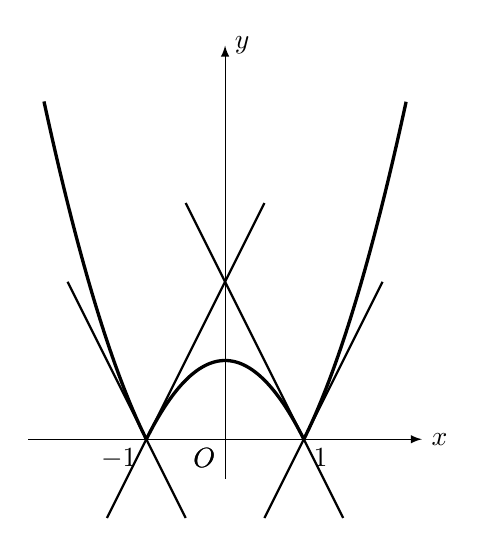
\begin{tikzpicture}[>=latex, scale=1]
    \draw[->](-2.5,0)--(2.5,0)node[right]{$x$};
    \draw[->](0,-.5)--(0,5)node[right]{$y$};
    \node at (0,0)[below left]{$O$};
    \draw[domain=-2.3:-1, samples=100, very thick]plot(\x, {\x*\x-1});
    \draw[domain=1:2.3, samples=100, very thick]plot(\x, {\x*\x-1});
    \draw[domain=-1:1, samples=100, very thick]plot(\x, {-\x*\x+1});
    \node at (0,0)[below left]{$O$};
    \node at (-1,0)[below left]{$-1$};
    \node at (1,0)[below right]{$1$};
    
    \draw[domain=-2:-.5, samples=10, thick]plot(\x, {-2*\x-2});
    \draw[domain=-1.5:.5, samples=10, thick]plot(\x, {2*\x+2});
    \draw[domain=-.5:1.5, samples=10, thick]plot(\x, {-2*\x+2});
    \draw[domain=.5:2, samples=10, thick]plot(\x, {2*\x-2});

\end{tikzpicture}
    \caption{}\label{fig:f(x)=|x^2-1|}
\end{figure}
    
\begin{solution}
函数$f(x)=|x^2-1|$是一个到处连续的函数,它的图象如图\ref{fig:f(x)=|x^2-1|}所示.

去掉函数式中的绝对值的符号,$f(x)$便可以写成分段函数式:
\[f(x)=\begin{cases}
    x^2-1,& x\le -1\quad \text{或}\quad x\ge 1\\
    -(x^2-1), & -1\le x\le 1
\end{cases}\]
所以
\[f'(x)=\begin{cases}
    2x ,&  x< -1\quad \text{或}\quad x> 1\\
    -2x,& -1<x<1
\end{cases}\]
但是当$x=-1$和1时,函数$f(x)$的左导数和右导数不相等,即此时导数不存在.因为当$x=-1$时,函数$f(x)$在$-1$点左邻域的表达式是
\[f (x) =x^2-1\]
而在$-1$点右邻域的表达式是
\[f (x) =- (x^2-1)\]
所以$f(x)$在$x=-1$点的左导数是
\begin{align*}
    f'_-(-1)&=\lim_{\Delta x\to 0^-}\frac{f(-1+\Delta x)-f(-1)}{\Delta x}\\
    &=\lim_{\Delta x\to 0^-}\frac{[(-1+\Delta x)^2-1]-0}{\Delta x}\\
    &=\lim_{\Delta x\to 0^-}(-2+\Delta x)=-2
\end{align*}
$f(x)$在$x=-1$点的右导数是
\begin{align*}
    f'_+(-1)&=\lim_{\Delta x\to 0^+}\frac{f(-1+\Delta x)-f(-1)}{\Delta x}\\
    &=\lim_{\Delta x\to 0^+}\frac{-[(-1+\Delta x)^2-1]-0}{\Delta x}\\
    &=\lim_{\Delta x\to 0^+}(2-\Delta x)=2 
\end{align*}
由于$f'_-(-1)\ne f'_+(-1)$, 所以我们说$f(x)$在$x=-1$处的导数不存在,同样可得
\[-2=f'_- (1)\ne f'_+(1)=2\]
故$f(x)$在$x=1$处也不可微.

因此,$f(x)=|x^2-1|$的导函数的定义域是$x\ne\pm 1$的点的集合,它的函数值如下:
\[f'(x)=\begin{cases}
    2x,& |x|>1\\
    -2x,& |x|<1
\end{cases}\]
\end{solution}

对照图\ref{fig:f(x)=|x^2-1|}来看,尽管函数$f(x)=|x^2-1|$处处连续,但是在$x=-1$和1这两点,曲线的特征是当动点由左侧趋于定
点1(或$-1$)时,割线的极限位置存在;当动点由右侧趋于定点1(或$-1$)时,割线的极限位置也存在,这两个极限位置分别叫1(或$-1$)点的\textbf{左、右切线},并且它们之间的夹角不为\textbf{平角},点$-1$和1分别是曲线的一种\textbf{角点}.
    
图\ref{fig:vertical_tangent}的情形是曲线$y=f(x)$在$P(x_0,y_0)$点连续并且在此点有平行于$y$轴的切线.现在我们来讨论图\ref{fig:vertical_tangent}中所示各函数在点$x_0$处的导数:

\begin{figure}[htp]
    \centering
\begin{tikzpicture}[>=latex]
\begin{scope}
\draw[->](-.5,0)--(4,0)node[right]{$x$};
\draw[->](0,-.5)--(0,4)node[right]{$y$};
\node at (2,-1){(a)};
\node at (0,0)[below left]{$O$};
\draw(2,0)node[below]{$x_0$}--(2,3.5);
\node at (2,2)[right]{$P(x_0,y_0)$};
\tkzDefPoints{1.5/.2/A, 2/2/B, 2.5/3.8/C}
\draw[very thick](A) to [bend right=18] (B) to [bend left=18](C);

\end{scope}
\begin{scope}[xshift=6cm]
    \draw[->](-.5,0)--(4,0)node[right]{$x$};
\draw[->](0,-.5)--(0,4)node[right]{$y$};
\node at (2,-1){(b)};
\node at (0,0)[below left]{$O$};
\draw(2,0)node[below]{$x_0$}--(2,3.5);
\node at (2,2)[right]{$P(x_0,y_0)$};
\tkzDefPoints{2.5/.2/A, 2/2/B, 1.5/3.8/C}
\draw[very thick](A) to [bend right=-18] (B) to [bend left=-18](C);

\end{scope}
\begin{scope}[yshift=-6cm]
    \draw[->](-.5,0)--(4,0)node[right]{$x$};
\draw[->](0,-.5)--(0,4)node[right]{$y$};
\node at (2,-1){(c)};
\node at (0,0)[below left]{$O$};
\draw(2,0)node[below]{$x_0$}--(2,3.5);
\node at (2,2)[right]{$P(x_0,y_0)$};
\tkzDefPoints{1.5/.2/A, 2/2/B, 2.5/.2/C}
\draw[very thick](A) to [bend right=18] (B) to [bend left=-18](C);


\end{scope}

\begin{scope}[xshift=6cm, yshift=-6cm]
    \draw[->](-.5,0)--(4,0)node[right]{$x$};
\draw[->](0,-.5)--(0,4)node[right]{$y$};
\node at (2,-1){(d)};
\node at (0,0)[below left]{$O$};
\draw(2,0)node[below]{$x_0$}--(2,3.5);
\node at (2,2)[right]{$P(x_0,y_0)$};
\tkzDefPoints{1.5/3.8/A, 2/2/B, 2.5/3.8/C}
\draw[very thick](A) to [bend right=-18] (B) to [bend left=18](C);



\end{scope}
\end{tikzpicture}
    \caption{}\label{fig:vertical_tangent}
\end{figure}

图(a)表示的函数在点$x_0$的邻近递增,因此过曲线上$P(x_0,y_0)$和$Q(x_0+\Delta x,y_0+\Delta y)$两点的割线,无论$Q$点在$P$点的哪一侧,$\Delta x$与$\Delta y$都有相同正、负号,于是
\[\frac{\Delta y}{\Delta x}=\frac{f(x_0+\Delta x)-f(x_0)}{\Delta x}>0\]
而且当$\Delta x\to 0$时,割线的倾斜角$\varphi$($0^{\circ}\le \varphi\le 180^{\circ}$)便以$\pi/2$为极限,从而
\[\lim_{\Delta x\to 0}\frac{f(x_0+\Delta x)-f(x_0)}{\Delta x}=\lim_{\varphi\to \tfrac{\pi^-}{2}}\tan\varphi=+\infty\]
可见$f(x)$在点$x_0$不可微(不存在有限导数),但是我们常常把这种情况:当$\Delta x\to 0$时,$\frac{\Delta y}{\Delta x}\to\infty$简略地叙述为函
数$f(x)$在$x_0$的导数为正无穷大,记作$f'(x_0)=+\infty$.

图(b)表示的函数$f$在点$x_0$的邻近递减,因此过曲线上$P(x_0,y_0)$和$Q(x_0+\Delta x,y_0+\Delta y)$两点的割线,无论$Q$点在$P$点的哪一侧,$\Delta x$与$\Delta y$都有相反的正、负号,于是
\[\frac{\Delta y}{\Delta x}=\frac{f(x_0+\Delta x)-f(x_0)}{\Delta x}<0\]
而且当$\Delta x\to 0$时,$\varphi\to \frac{\pi^+}{2}$,从而
\[\lim_{\Delta x\to 0}\frac{f(x_0+\Delta x)-f(x_0)}{\Delta x}=\lim_{\varphi\to \tfrac{\pi^+}{2}}\tan\varphi=-\infty\]
因此$f(x)$在点$x_0$处不可微,但是我们常常把这种情况叙述为函数$f(x)$在$x_0$处的导数为负无穷大,记作$f'(x_0)=-\infty$.

图\ref{fig:vertical_tangent}(c)表示的函数在点$x_0$处连续,让$x$由$x_0$变动到
$x_0+\Delta x$,于是由$\Delta x$所引起的相应的函数的改变量$\Delta y$的情形是:
\begin{itemize}
    \item 当$\Delta x<0$时,有$\Delta y<0$,从而$\frac{\Delta y}{\Delta x}>0$;
    \item 当$\Delta x>0$时,有$\Delta y<  0$,从而$\frac{\Delta y}{\Delta x}<0$.
\end{itemize}
于是:
\begin{itemize}
    \item 当$\Delta x\to 0^-$时,$\varphi\to \frac{\pi^-}{2}$,从而$\frac{\Delta y}{\Delta x}=\tan\varphi\to +\infty$;
    \item 当$\Delta x\to 0^+$时,$\varphi\to \frac{\pi^+}{2}$,从而$\frac{\Delta y}{\Delta x}=\tan\varphi\to -\infty$.
\end{itemize}
因此$f(x)$在点$x_0$不可微,但是我们常把这种情况叙述为$f(x)$在点$x_0$的左导数$f'_-(x_0)=+\infty$, 而它的右导数为$f'_+(x_0)=-\infty$, 曲线在$x_0$处由上升转为下降有一个尖点,它的切线垂直于$x$轴.

图(d)表示的函数在点$x_0$处连续,但是
\begin{itemize}
    \item 当$\Delta x\to 0^-$时,$\frac{\Delta y}{\Delta x}=\tan\varphi\to -\infty$;
    \item 当$\Delta x\to 0^+$时,$\frac{\Delta y}{\Delta x}=\tan\varphi\to +\infty$.
\end{itemize}
因此,$f(x)$在点$x_0$不可微,我们常常把这种情况叙述为$f'_-(x_0)=-\infty$和$f'_+(x_0)=+\infty$, 点$x_0$是曲线的一个尖点,它的切线垂直于$x$轴.

\begin{example}
设$f(x)=\begin{cases}
    0,& x=0\\
    x\sin\frac{1}{x},& x\ne 0
\end{cases}$

讨论它在0点的导数.
\end{example}

\begin{solution}
在第一章,我们已经说明了
\[\lim_{x\to 0}x\sin\frac{1}{x}=0=f(0)\]
因此,$f(x)$在点$x=0$连续,很明显$f(x)$在其它各点处也都连续,所以说$f(x)$是一个到处连续的函数,我们将说明它在原点不存在导数.

因为
\[\frac{f(0+\Delta x)-f(0)}{\Delta x}=\frac{\Delta x\sin\frac{1}{\Delta x}}{\Delta x}=\sin\frac{1}{\Delta x}\]
而当$\Delta x\to 0$时,$\sin\frac{1}{\Delta x}$
没有极限,故$f'(0)$不存在,就
其几何意义来说,当动点沿着曲线$y=x\sin\frac{1}{x}$趋于原点$O$
时,割线$OQ$不断地在$-\frac{\pi}{4}\le \theta\le \frac{\pi}{4}$这个幅度之内摆动,而不趋于任何极限位置,即切线不存在(图\ref{fig:x*sin(1/x)}).
\end{solution}

\begin{figure}[htp]
    \centering
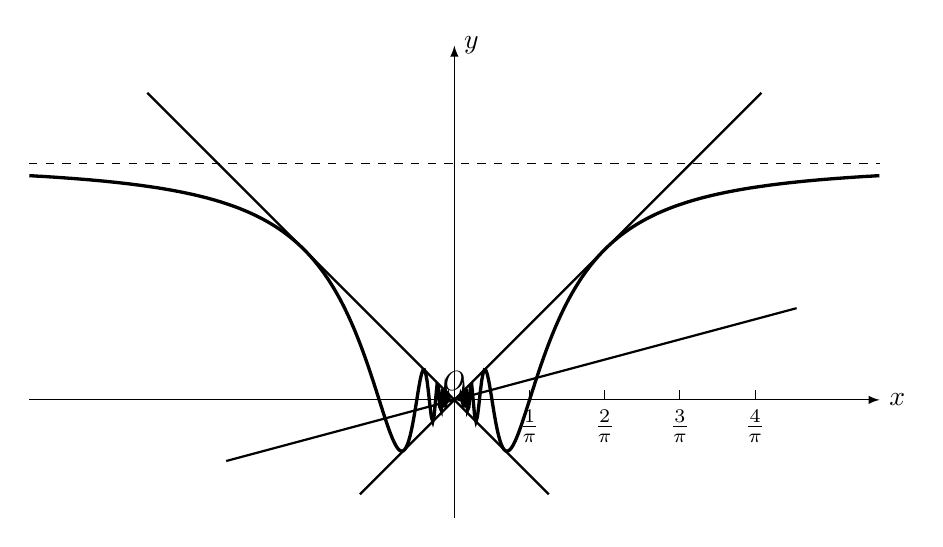
\begin{tikzpicture}[>=latex, scale=3]
\draw[->](-1.8,0)--(1.8,0)node[right]{$x$};
\draw[->](0,-.5)--(0,1.5)node[right]{$y$};
\draw[domain=.02:1.8, very thick, samples=300]plot(\x, {\x*sin(1/\x r)});
\draw[domain=.02:1.8, very thick, samples=300]plot(-\x, {\x*sin(1/\x r)});
\draw[thick](-.4,-.4)--(1.3,1.3);
\draw[thick](.4,-.4)--(-1.3,1.3);
\draw[thick](15:1.5)--(-165:1);
\draw[dashed](-1.8,1)--(1.8,1);

\foreach \x in {1,2,3,4}
{
   \draw(\x/pi,0)node[below]{$\frac{\x}{\pi}$}--(\x/pi,.04);
}

\node at (0,0)[above]{$O$};
\end{tikzpicture}
    \caption{}\label{fig:x*sin(1/x)}
\end{figure}

通过以上的例子,我们知道函数的连续点未必是它的可以微分点.几种常见的不可微分点如例2.4的角点,平行于$y$轴的切线的切点,特别是曲线上的尖点和在例2.5的曲线上的不存在割线的极限位置的点.

假如区间$[a,b]$上的函数$f(x)$, 在开区间$(a,b)$中存在着导数$f'(x)$, 并且$f'_+(a)$和$f'_-(b)$都存在,则称$f(x)$在闭区间上可以微分(可导).

\begin{ex}
\begin{enumerate}
    \item 说明下面函数在点$x=0$不可微:
\begin{multicols}{2}
\begin{enumerate}
    \item $f(x)=|x|$
    \item $f(x)=\begin{cases}
        x^2,& x\le 0\\
        x,& x\ge 0
    \end{cases}$
    \item $f(x)=\sqrt[3]{x}$
    \item $f(x)=\sqrt{|x|}$
\end{enumerate}
\end{multicols}
\item 说明函数$f(x)=\begin{cases}
    x^2,& x\ge 0\\
    -x^2,& x<0
\end{cases}$
    处处可微.
\item \begin{enumerate}
\item 假设$g(x)=f(x+c)$. 从定义出发证明$g'(x)=f'(x+c)$, 并绘图说明.    
\item 设$f$可微并有周期$\varphi$, 证明$f'$也是有周期的.
\end{enumerate}

\end{enumerate}
\end{ex}

\section{微商运算的基本法则}
\subsection{几个基本函数的微商(导数)}
\subsubsection{常数函数的导数恒等于0}

\begin{proof}
设$f(x)=c$ ($c$是常数),则根据常数函数的性质,由自变数$x$的改变量$\Delta x$引起的相应的函数的改变量为:
\[\Delta y=f (x+\Delta x) -f (x)=c-c=0\]
显然差商$\frac{\Delta y}{\Delta x}=\frac{0}{\Delta x}=0$, 故
\[f' (x) =\lim_{\Delta x\to 0}\frac{\Delta y}{\Delta x}=
\lim_{\Delta x\to 0} 0=0\]
这个事实是明显的,因为当自变数$x$有增、减时,函数值并无增、减,因此,它的变化率为零.
\end{proof}

\subsubsection{一次函数(直线函数)的导数是常数}

若$f(x)=kx+b$, 则$f'(x)=k$. 

\subsubsection{若$f(x)=x^n$ ($n$是正整数),则$f'(x)=nx^{n-1}$}

\begin{proof}
  由自变量的改变量$\Delta x$引起的函数改变量为
\[\Delta y=f (x+\Delta x) -f (x) = (x+\Delta x)^n-x^n\] 
按牛顿二项式定理展开,得  
\begin{align*}
\Delta y&= x^n+nx^{n-1}\Delta x+\frac{n(n-1)}{1\cdot 2}x^{n-2}(\Delta x)^2+\cdots+nx(\Delta x)^{n-1}+(\Delta x)^n-x^n\\
&=nx^{n-1}\Delta x+\frac{n(n-1)}{1\cdot 2}x^{n-2}(\Delta x)^2+\cdots+nx(\Delta x)^{n-1}+(\Delta x)^n
\end{align*}
其中差商
\[\frac{\Delta y}{\Delta x}=nx^{n-1}+\frac{n(n-1)}{1\cdot 2}x^{n-2}\Delta x+\cdots+nx(\Delta x)^{n-2}+(\Delta x)^{n-1}\]
式中除第一项外,其余各项随$\Delta x\to 0$而趋于0,因此:
\[f'(x)=\lim_{\Delta x\to 0}\frac{\Delta y}{\Delta x}=nx^{n-1}\]
\end{proof}

\subsubsection{若$f(x)=x^{\mu}$ (其中$\mu$是任意实数,函数的定义域依赖于$\mu$), 则$f'(x)=\mu x^{\mu-1}$}

\begin{proof}
    \[\frac{\Delta y}{\Delta x}=\frac{(x+\Delta x)^{\mu}-x^{\mu}}{\Delta x}=x^{\mu-1}\cdot \frac{\left(1+\frac{\Delta x}{x}\right)^{\mu-1}}{\frac{\Delta x}{x}}\]
利用第一章中已经算出的极限
\[\lim_{x\to 0}\frac{(1+x)^{\mu}-1}{x}=\mu\]
就得到
\[f'(x)=\lim_{\Delta x\to 0}\frac{\Delta y}{\Delta x}=\mu x^{\mu-1}\]
\end{proof}

特殊情形:
\begin{enumerate}
    \item 若$f(x)=\frac{1}{x}=x^{-1},\; (x\ne 0)$,则$f'(x)=(-1)x^{-2}=-\frac{1}{x^2}$
    \item 若$f(x)=\sqrt{x}=x^{\tfrac{1}{2}},\; (x\ge 0)$,则$f'(x)=\frac{1}{2}x^{-\tfrac{1}{2}}=\frac{1}{2\sqrt{x}}$
\end{enumerate}

\subsubsection{若$f(x)=\log_a x\; (0<a\ne 1,\; 0<x<+\infty)$,则$f'(x)=\frac{\log_a e}{x}$}

\begin{proof}
\begin{align*}
    \frac{\Delta y}{\Delta x}&=\frac{\log_a(x+\Delta x)-\log_a x}{\Delta x}\\
    &=\frac{1}{x}\cdot \frac{\log_a\left(1+\frac{\Delta x}{x}\right)}{\frac{\Delta x}{x}}\\
    &=\frac{1}{x}\cdot \log_a\left(1+\frac{\Delta x}{x}\right)^{\tfrac{1}{\Delta x/x}}
\end{align*}  

利用极限$\Lim_{t\to 0}(1+t)^{1/t}=e$,以及对数函数是连续函数,得到
\begin{align*}
    f'(x)&=\lim_{\Delta x\to 0}\frac{\Delta y}{\Delta x}=\frac{1}{x}\lim_{\tfrac{\Delta x}{x}\to 0}\log_a\left(1+\frac{\Delta x}{x}\right)^{\tfrac{1}{\Delta x/x}}\\
    &=\frac{1}{x}\log_a\left[\lim_{\tfrac{\Delta x}{x}\to 0}\left(1+\frac{\Delta x}{x}\right)^{\tfrac{1}{\Delta x/x}}\right]\\
    &=\frac{1}{x}\log_a e=\frac{\log_a e}{x}
\end{align*}

特别:当$f(x)=\ln x$时,$f'(x)=\frac{1}{x}$.
\end{proof}

上面的结果表明对数函数($a>1$时)的增大速度是与自
变数的值成反比的,当自变数无限增大时,增大速度就保持正值而趋向于0. 由于自然对数的导数比较简单,所以在理论研究中常常采用自然对数.

\subsubsection{若$f(x)=a^x\; (0<a\ne 1,\; -\infty<x<+\infty)$,则$f'(x)=a^x\cdot \ln a$}

\begin{proof}
    \[\frac{\Delta y}{\Delta x}=\frac{a^{x+\Delta x}-a^x}{\Delta x}=a^x\cdot \frac{a^{\Delta x}-1}{\Delta x}\]
利用$\Lim_{\Delta x\to 0}a^{\Delta x}=1$,则可设$a^{\Delta x}=1+\alpha$,且当$\Delta x\to 0$时,有$\alpha\to 0$. 在此等式的两边取对数,得:
\[\Delta x=\log_a(1+\alpha)\]
于是
\[\frac{\Delta y}{\Delta x}=a^x\cdot \frac{\alpha}{\log_a(1+\alpha)}=a^x\cdot \frac{1}{\log_a(1+\alpha)^{1/\alpha}}\]
因此
\begin{align*}
    f'(x)&=\lim_{\Delta x\to 0}\frac{\Delta y}{\Delta x}=a^x\cdot \frac{1}{\Lim_{\alpha\to 0}\log_a(1+\alpha)^{1/\alpha}}\\
    &=a^x\cdot \frac{1}{\log_a\left[\Lim_{\alpha\to 0}(1+\alpha)^{1/\alpha}\right]}\\
    &=a^x\cdot \frac{1}{\log_a e}
\end{align*}
又因为$\ln a=\frac{1}{\log_a e}$,所以
\[f'(x)=a^x\cdot \ln a\]

特别,若$f(x)=e^x$,则$f'(x)=e^x$.
\end{proof}

这个事实表明指数函数(当$a>1$时)的增大速度与函数值成正比例,当底数为$e$时,导数的结果特别简单.


\subsubsection{若$f(x)=\sin x$, 则$f'(x)=\cos x$}
\begin{proof}
    \begin{align*}
\frac{\Delta y}{\Delta x}&=\frac{\sin(x+\Delta x)-\sin x}{\Delta x}\\
&=\frac{2\cos\left(x+\frac{\Delta x}{2}\right)\sin\frac{\Delta x}{2}}{\Delta x}\\
&=\cos\left(x+\frac{\Delta x}{2}\right)\cdot \frac{\sin\frac{\Delta x}{2}}{\frac{\Delta x}{2}}
    \end{align*}
因此
\begin{align*}
    \lim_{\Delta x\to 0}\frac{\Delta y}{\Delta x}&=\lim_{\Delta x\to 0}\left[\cos\left(x+\frac{\Delta x}{2}\right)\cdot \frac{\sin\frac{\Delta x}{2}}{\frac{\Delta x}{2}}\right]\\
    &=\lim_{\Delta x\to 0}\cos\left(x+\frac{\Delta x}{2}\right)\cdot \lim_{\Delta x/2\to 0}\frac{\sin\frac{\Delta x}{2}}{\frac{\Delta x}{2}}
\end{align*}
根据$\cos x$的连续性与极限$\Lim_{t\to 0}\frac{\sin t}{t}=1$, 得到
$f' (x) =\cos x$.
\end{proof}

\subsubsection{若$f(x)=\cos x$, 则$f'(x)=-\sin x$}
\begin{proof}
\begin{align*}
\frac{\Delta y}{\Delta x}&=\frac{\cos(x+\Delta x)-\cos x}{\Delta x}\\
&=\frac{-2\sin\left(x+\frac{\Delta x}{2}\right)\cdot \sin\frac{\Delta x}{2}}{\Delta x}\\
&=-\sin\left(x+\frac{\Delta x}{2}\right)\cdot \frac{\sin\frac{\Delta x}{2}}{\frac{\Delta x}{2}}
    \end{align*}
因此
\begin{align*}
    \lim_{\Delta x\to 0}\frac{\Delta y}{\Delta x}&=-\lim_{\Delta x\to 0}\left[\sin\left(x+\frac{\Delta x}{2}\right)\cdot \frac{\sin\frac{\Delta x}{2}}{\frac{\Delta x}{2}}\right]\\
    &=-\lim_{\Delta x\to 0}\sin\left(x+\frac{\Delta x}{2}\right)\cdot \lim_{\Delta x/2\to 0}\frac{\sin\frac{\Delta x}{2}}{\frac{\Delta x}{2}}\\
    &=-\sin  x
\end{align*}
\end{proof}

现在将上面的导数公式列成下表:
\begin{enumerate}
    \item $\frac{\dd c}{\dd x}=0$
    \item $\frac{\dd(kx+b)}{\dd x}=k$
    \item $\frac{\dd x^n}{\dd x}=nx^{n-1}$\quad ($n$为自然数)
    \item $\frac{\dd x^\mu}{\dd x}=\mu x^{\mu-1}$\quad ($\mu$为任意实数)
    \item $\frac{\dd\log_a x}{\dd x}=\frac{\log_a e}{x},\qquad \frac{\dd \ln x}{\dd x}=\frac{1}{x}$
    \item $\frac{\dd a^x}{\dd x}=a^x\cdot \ln a,\qquad \frac{\dd e^x}{\dd x}=e^x$
    \item $\frac{\dd\sin x}{\dd x}=\cos x,\qquad \frac{\dd \cos x}{\dd x}=-\sin x$
\end{enumerate}

\subsection{求导的基本法则}

现在要建立一些求导数的公式,用这些公式等函数的导数.

\begin{blk}
{定理1} 函数和的导数等于各函数的导数的和,即:
\[[f (x) +g (x) ] '=f' (x) +g' (x)\] 
\end{blk}

\begin{proof}
    设$u(x)=f(x)+g(x)$, 任意固定$x$, 作取非零数$\Delta x$,有 
\begin{align*}
    \frac{\Delta u(x)}{\Delta x}&=\frac{[f(x+\Delta x)+g(x+\Delta x)]-[f(x)+g(x)]}{\Delta x}\\
    &=\frac{f(x+\Delta x)-f(x)}{\Delta x}+\frac{g(x+\Delta x)-g(x)}{\Delta x}\\
    &=\frac{\Delta f(x)}{\Delta x}+\frac{\Delta g(x)}{\Delta x}
\end{align*}
令$\Delta x\to 0$,即得:
\begin{align*}
    [f(x)+g(x)]'&=\lim_{\Delta x\to 0}\frac{\Delta u(x)}{\Delta x}\\
    &=\lim_{\Delta x\to 0}\frac{\Delta f(x)}{\Delta x}+\lim_{\Delta x\to 0}\frac{\Delta g(x)}{\Delta x}\\
    &=f'(x)+g'(x)
\end{align*}
\end{proof}

这个法则可以推广到任意有限个函数.

\begin{blk}
{定理2} $[A\varphi (x)]'=A\varphi'(x)$, 其中$A$是常数,即常因数不因微分法而改变.    
\end{blk}

\begin{proof}
设$f(x)=A\varphi(x)$, 
\begin{align*}
    [A\varphi(x)]'&=f'(x)=\lim_{\Delta x\to 0}\left[A\frac{\varphi(x+\Delta x)-\varphi(x)}{\Delta x}\right]\\
    &=A\lim_{\Delta x\to 0}\frac{\varphi(x+\Delta x)-\varphi(x)}{\Delta x}\\
    &=A\varphi'(x)
\end{align*}
\end{proof}

\begin{example}
    求$3x^2-7x-1$的导数.
\end{example}

\begin{solution}
\[  (3x^2-7x-1)'=(3x^2)'+(-7x)'+(-1)'=6x-7\]
\end{solution}    

\begin{blk}{推论}
设$f(x)=a_nx^n+a_{n-1}x^{n-1}+\cdots+a_1x+a_0\; (a_n\ne 0)$,则
\[f'(x)=na_nx^{n-1}+(n-1)a_{n-1}x^{n-2}+\cdots+a_1\]
\end{blk}

\begin{example}
求过抛物线$y=3x^2+6$外一点$P(2,-9)$所引抛物线的两条切线的方程.
\end{example}

\begin{solution}
在点$x$处的抛物线的切线的斜率为
\[k=y'_x=6x\]
故过抛物线上一点$T(x_1,y_1)$的切线方程为
\[y-y_1=6x_1 (x-x_1)\] 

$\because\quad y_1=3x^2_1+6$

$\therefore\quad $切线方程可化简为
\[    y=6x_1x-3x_1^2+6\]
设切线通过$P(2,-9)$点,于是
\[9=12x_1-3x_1^2+6\]
即:$x_1^2-4x_1-5=0$

$\therefore\quad x_1=-1$或$5$,从而$y_1=9$或81.

故所求切线方程为:
\[y-9=-6(x+1)\quad\text{和}\quad y-81=30(x-5)\]
即:
\[y+6x-3=0\quad\text{和}\quad  y-30x+69=0\]
\end{solution}

\begin{example}
求三次函数$f(x)=ax^3+3bx^2+3cx+d$的图象与$x$轴相切的条件.
\end{example}

    
\begin{solution}
由函数$f(x)=ax^3+3bx^2+3cx+d$求得它的图象任意一点$x=x_0$处的切线斜率为
\[f' (x) =3ax^2_0+6bx_0+3c=3 (ax^2_0+2bx_0+c) \]
    
要此曲线与$x$轴相切于$(x_0,0)$点,$x_0$必须满足条件
\begin{numcases}{}
    ax^3_0+3bx^2_0+3cx_0+d=0\\
    ax^2_0+2bx_0+c=0
\end{numcases}
将(2.1)改写成
\begin{equation}
    x_0(ax^2_0+2bx_0+c)+bx_0^2+2cx_0+d=0
\end{equation}
(2.2)代入得
\begin{equation}
    bx_0^2+2cx_0+d=0
\end{equation}
于是解(2.1)和(2.2)即解(2.2)和(2.4),要方程(2.2)和(2.4)有公共解,必须
\[D=\begin{vmatrix}
    a&2b\\b&2c
\end{vmatrix}=2(ac-b^2)\ne 0\]
于是
\[x^2_0=\frac{c^2-bd}{b^2-ac},\qquad x_0=\frac{ad-bc}{2(b^2-ac)}\; (b^2-ac\ne 0)\]
所以,$a,b,c,d$必须适合条件
\[\begin{cases}
    b^2-ac\ne 0\\
    \frac{c^2-bd}{b^2-ac}=\frac{(ad-bc)^2}{4(b^2-ac)^2}
\end{cases}\]
即
\[\begin{cases}
    b^2-ac\ne 0\\
   (ad-bc)^2 =4(b^2-ac)(c^2-bd)
\end{cases}\]
\end{solution}

\begin{blk}
    {定理3} 二函数之积的导数为两项之和,其中第一项是第一个因子的导数与第二个因子的乘积,而第二项是第二个因子的导数与第一个因子的乘积,即
\[[f (x) \cdot g (x) ] '=f' (x) \cdot g (x) +f (x) \cdot g' (x) \]
\end{blk}

\begin{proof}
    设 $h(x)=f(x)\cdot g(x)$, 任取非零数$\Delta x$, 则
\begin{align*}
    [f(x)\cdot g(x)]'&=\lim_{\Delta x\to 0}\frac{\Delta h(x)}{\Delta x}\\
    &=\lim_{\Delta x\to 0}\frac{f(x+\Delta x)g(x+\Delta x)-f(x)g(x)}{\Delta x}\\
    &=\lim_{\Delta x\to 0}\frac{1}{\Delta x}\Bigl[f(x+\Delta x)g(x+\Delta x)-f(x)g(x+\Delta x)\\
    &\qquad\qquad +f(x)g(x+\Delta x)-f(x)g(x) \Bigr]\\
    &=\lim_{\Delta x\to 0}\frac{f(x+\Delta x)-f(x)}{\Delta x}\cdot g(x+\Delta x)\\
    &\qquad +\lim_{\Delta x\to 0}f(x)\cdot \frac{g(x+\Delta x)-g(x)}{\Delta x}\\
    &=f' (x) \cdot g (x) +f (x) \cdot g' (x) 
\end{align*}
\end{proof}

重复应用这个定理,我们便可以求两个以上的函数之积的导数,例如
\[\frac{\dd }{\dd x}(uvw)=(vw)\frac{\dd u}{\dd x}+u\frac{\dd }{\dd x}(vw)\]
但是
\[\frac{\dd }{\dd x}(vw)=w\frac{\dd v}{\dd x}+v\frac{\dd w}{\dd x}\]
代入上式便得到
\[\frac{\dd }{\dd x}(uvw)=vw\frac{\dd u}{\dd x}+uw\frac{\dd v}{\dd x}+uv\frac{\dd w}{\dd x}\]


\begin{example}
    设$f(x)=\sqrt{x}(x^2-3)$,求$f'(x)$
\end{example}


\begin{solution}
    \begin{align*}
f'(x)&=\left[\sqrt{x}(x^2-3)\right]'\\
&=\left(\sqrt{x}\right)'(x^2-3)+\sqrt{x}(x^2-3)'\\
&=\frac{7}{2\sqrt{x}}(x^2-3)+\sqrt{x}\cdot 2x = \frac{5x^2-3}{2\sqrt{x}}
    \end{align*}
\end{solution}

\begin{example}
    设$f(x)=\frac{1}{2}\sin^2 x+x\sin x+\frac{7}{x^2}$,求$f'(x)$
\end{example}

\begin{solution}
\begin{align*}
    f'(x)&=\left(\frac{1}{2}\sin^2 x\right)'+(x\sin x)'+\left(\frac{7}{x^2}\right)'\\
    &=\frac{1}{2}\left[(\sin x)'\sin x+\sin x(\sin x)'\right]+(\sin x+x\cos x)-\frac{14}{x^3}\\
    &=\sin x\cos x+\sin x+x\cos x-\frac{14}{x^3}
\end{align*}
\end{solution}

\begin{blk}
    {定理4} 两个函数的商的导数,等于分子的导数与分母的积,减去分母的导数与分子的积,再除以分母的平方,即
\[\left(\frac{u(x)}{v(x)}\right)'=\frac{v(x)\cdot u'(x)-u(x)\cdot v'(x)}{[v(x)]^2}\]
\end{blk}

\begin{proof}
    设$f(x)=\frac{u(x)}{v(x)}$,任取非零数$\Delta x$,则
\begin{align*}
    \left(\frac{u(x)}{v(x)}\right)'&=\lim_{\Delta x\to 0}\frac{\Delta f(x)}{\Delta x}=\lim_{\Delta x\to 0}\frac{\frac{u(x+\Delta x)}{v(x+\Delta x)}-\frac{u(x)}{v(x)}}{\Delta x}\\
    &=\lim_{\Delta x\to 0}\frac{1}{\Delta x}\left\{\frac{u(x+\Delta x)\cdot v(x)-u(x)\cdot v(x+\Delta x)}{v(x+\Delta x)\cdot v(x)}\right\}\\
    &=\lim_{\Delta x\to 0}\frac{1}{\Delta x}\left\{\frac{v(x)[u(x+\Delta x)-u(x)]}{v(x)v(x+\Delta x)}-\frac{u(x)[v(x+\Delta x)-v(x)]}{v(x)v(x+\Delta x)}\right\}\\
    &=\frac{v(x)\Lim_{\Delta x\to 0}\frac{u(x+\Delta x)-u(x)}{\Delta x}}{v(x)\Lim_{\Delta x\to 0}v(x+\Delta x)}-\frac{u(x)\Lim_{\Delta x\to 0}\frac{v(x+\Delta x)-v(x)}{\Delta x}}{v(x)\Lim_{\Delta x\to 0}v(x+\Delta x)}\\
    &=\frac{v(x) u'(x)-u(x) v'(x)}{v^2(x)}
\end{align*}
\end{proof}


\begin{example}
求证:$(\tan x)'=\sec^2 x,\qquad (\cot x)'=-csc^2 x$
\end{example}

\begin{proof}    
\begin{align*}
    (\tan x)'&=\left(\frac{\sin x}{\cos x}\right)'\\
    &=\frac{\cos x(\sin x)'-\sin x(\cos x)'}{\cos^2 x}\\
    &=\frac{\cos^2 x+\sin^2 x}{\cos^2x}\\
    &=\frac{1}{\cos^2 x}=\sec^2 x
\end{align*}
\[(\cot x)'=\left(\frac{\cos x}{\sin x}\right)'=\frac{-\sin^2 x-\cos^2 x}{\sin^2 x}=-\csc^2 x\]    
\end{proof}

\begin{example}
    求$\left(\frac{2x-1}{x^2+1}\right)'$
\end{example}

\begin{solution}
\begin{align*}
    \left(\frac{2x-1}{x^2+1}\right)'&=\frac{(x^2+1)(2x-1)'-(2x-1)(x^2+1)'}{(x^2+1)^2}\\
&=\frac{(x^2+1)\cdot 2-(2x-1)(2x)}{(x^2+1)^2}\\
&=\frac{2(x^2+1)-(4x^2-2x)}{(x^2+1)^2}\\
&=\frac{-2(x^2-x-1)}{(x^2+1)^2}
\end{align*}
\end{solution}

\begin{ex}
\begin{enumerate}
    \item  求下面各函数的导函数:
\begin{multicols}{2}
\begin{enumerate}
    \item $3 x^{3}-1$
    \item  $x+2 x^{2}+3 x^{3}$
    \item  $1-\frac{1}{x^{2}}$
    \item $\frac{x^{2}+1}{x}$
    \item  $1+\frac{1}{x}-\frac{1}{x^{2}}$
    \item  $\frac{2 x^{5}-7 x^{3}-3 x^{2}}{6 x^{2}}$
    \item  $(x+2)\left(x^{2}+1\right)$
    \item  $x+\sqrt{x}$
    \item $x-\frac{1}{\sqrt{x}}$
    \item  $\frac{x+1}{\sqrt{x}}$
    \item  $\frac{2 x \sqrt{x}-x^{\tfrac{5}{2}}+3 x^{\tfrac{1}{2}}}{-\sqrt{x}}$ \item  $e^{x}-e^{-x}$
    \item $\frac{x^{n}-x^{-n}}{x} $
    \item $\sin x+\cos x$
    \item $\sin x-\cos x$
\end{enumerate}
\end{multicols}
\item  求下面各函数的导函数:
\begin{multicols}{2}
\begin{enumerate}
    \item $\left(x^{2}+1\right)^{3} \sqrt{x}$
    \item $\frac{x+1}{\sqrt{x}}$
    \item  $x \sin x$
    \item $x \cot  x$
    \item  $\frac{\tan  x}{x}$;
    \item  $x \log _{2} x+x^{2} \tan  x$
    \item  $\frac{x^{2}}{x^{3}+c^{3}}$
    \item  $x^{3} e^{-x}$;
    \item  $a^{-x} \sin x$ 
    \item $a^{x}\{(x+1) \cos x+\log_2 x\}$
    \item $\frac{\sqrt{x}+1}{2 x+1}$ 
    \item $\frac{2 x-1}{x^{2}+1}$
    \item $\frac{(x-3)(x-4)}{(x-5)}$
    \item  $\frac{x^{2}\left(x^{2}-1\right)\left(x^{3}-1\right)}{x+1}$
    \item  $\frac{x}{x+1}-\frac{1}{x-1}$
    \item  $x \sin x \cos x$
    \item $\sec x $ 
    \item $\csc x$
    \item $\frac{\sin x}{1+\tan  x}$
\end{enumerate}
\end{multicols}

\item 已知抛物线$y=x^2-x$上一点的切线平行于直线$y=x$.求此点的坐标.
\item 求曲线$y=x^3-x^2$上这样的点,使过该点的切线与$x$轴平行.
\item 若抛物线$y=ax^2+bx+c$通过原点,且过该点的切线的斜率等于2, 又抛物线过$(1, 1)$点,求$a$、$b$、$c$.
\item 对于函数$f(x)=x^3+ax^2+bx+c$, 方程$f(x)+\frac{1}{2}x=0$
有不相等的三根$2,\alpha,\beta$, 若$f'(\alpha)=f'(\beta)$, $f'(1)=0$, 求$a,b,c$.
\item 求三次函数$y=f(x)$, 使它同时满足下面的条件:
\begin{enumerate}
    \item 用$x+1$去除$f(x)$与用$(x-1)(x-2)$去除,$f(x)$所得余式相同;
    \item 过曲线$y=f(x)$上的点$(1,f(1))$的切线方程是
$y=-2x+1$
\end{enumerate}
\item 
过$(2, 0)$点求与曲线$y=\frac{1}{x}$相切的直线方程.
\item 
\begin{enumerate}
\item 在抛物线$y=x^2$上求这样一点,使过该点的切线与过$(a,a^2)$点的切线垂直;
\item 求抛物线两条正交切线交点的轨迹方程.
\end{enumerate}

\item 设抛物线方程为$y=x^2+ax+b$, 试问点$(x_0,y_0)$位于
何处时,可以从点$(x_0,y_0)$对此抛物线作出两条切线或一条切线,或作不出切线?
\item 求抛物线$y=x^2+ax$, $y=x^2+bx\; (a\ne b)$的公切线的方
程.
\end{enumerate} 
\end{ex}

\subsection{复合函数的求导法则}
\begin{blk}
    {定理} 假设函数$y=g(x)$在点$x$可导,而函数$z=f(y)$在点$g(x)$可导,那么复合函数$z=\varphi(x)=f(g(x))$在点$x$可导,并且
\[[f(g(x))]'=f'(g(x))\cdot g'(x)\]
简写成$[f(g(x))]'=f'_g\cdot g'_x$,或者写成
\[\frac{\dd z}{\dd x}=\frac{\dd z}{\dd y}\cdot \frac{\dd y}{\dd x}\]
\end{blk}

\begin{proof}
    设$D_g$, $D_f$分别是函数$g(x),f(y)$的定义域,令$x\in D_g$, $g(x)\in D_f$, 任取非零数$\Delta x$, 且使$g(x+\Delta x)\in D_f$,于是$\Delta g=g(x+\Delta x)-g(x)$, 又根据$g(x)$在点$x$连续,故当$x\to 0$时,$\Delta y\to 0$. 因为$g(x)$在点$x$可导,可以设
\begin{equation}
    \alpha=\frac{\Delta y}{\Delta x}-g'(x)
\end{equation}
而且由上式知道
\[\lim_{\Delta x\to 0}\alpha=\lim_{\Delta x\to 0}\left(\frac{\Delta y}{\Delta x}-g'(x)\right)=g'(x)-g'(x)=0\]
把(2.5)改写成
\begin{equation}
    \Delta y=g'(x)\Delta x+\alpha\Delta x
\end{equation}
其中$\alpha$随$\Delta x$一同趋向于零,且$\alpha \Delta x$是比$\Delta x$更小的量.

\begin{enumerate}
    \item 若$g'(x)\ne 0$,只要$\Delta x$够小,由(2.6)知$\Delta y\ne 0$,那么
\begin{align*}
    \frac{\varphi(x+\Delta x)-\varphi(x)}{\Delta x}&=\frac{f(g(x+\Delta x))-f(g(x))}{g(x+\Delta x)-g(x)}\cdot \frac{g(x+\Delta x)-g(x)}{\Delta x}\\
    &=\frac{f(g(x)+\Delta y)-f(g(x))}{\Delta y}\cdot \frac{\Delta y}{\Delta x}
\end{align*}
令$\Delta x\to 0$,由上式得
\[\varphi'(x)=f'(g(x))\cdot g'(x)\]
即
\[[f(g(x))]'=f'(g(x))\cdot g'(x)\]

\item 如果$g'(x)=0$,则当$\Delta x\to 0$时,有两种情形:
\begin{enumerate}
    \item 若$\Delta y=g(x+\Delta x)-g(x)=0$,则
\begin{align*}
    \frac{\varphi(x+\Delta x)-\varphi(x)}{\Delta x}&=\frac{f(g(x+\Delta x))-f(g(x))}{\Delta x}\\
    &=\frac{f(g(x))-f(g(x))}{\Delta x}=0
\end{align*}
\item 若$\Delta y\ne 0$,则
\[\frac{\varphi(x+\Delta x)-\varphi(x)}{\Delta x}=\frac{f(g(x+\Delta y))-f(g(x))}{\Delta y}\cdot \frac{\Delta y}{\Delta x}\]
令$\Delta x\to 0$,得到
\[\varphi'(x)f'(g(x))\cdot 0=0\]
\end{enumerate}
合并上述两种情形,都有
\[\varphi'(x)=[f(g(x))]'=0\]
于是定理得证.
\end{enumerate}
\end{proof}

这个定理是说:复合函数对自变量的导数,等于已知函数对中间变量的导数,乘以中间变量对自变量的导数.


\begin{example}
    设$\varphi (x)=2^{\sin x}$, 求$\varphi'(x)$.
\end{example}

    
\begin{solution}
    把$\varphi (x)$看成$u=\sin x$和$f(u)=2^u$的复合函数,于是$\varphi  (x) =2^{\sin x}=f (\sin x)$.

依上述定理,得
\begin{align*}
  \varphi' (x) &= [f (u) ]'\cdot u'_x= (2^u)'\cdot (\sin x)'\\
&=2^u\ln2 \cdot \cos x\\
&=2^{\sin x}\cdot \cos x \cdot \ln2  
\end{align*}
\end{solution}

\begin{example}
    设$y=\sin(x^2+x+1)\cdot \cos(x^3+2x^2)$, 求$y'_x$.
\end{example}

\begin{solution}
    设$u=x^2+x+1$, $v=x^3+2x^2$, 则
\begin{align*}
  y'&= (\sin u)'\cdot u'_x\cdot \cos v+\sin u\cdot (\cos v)'\cdot v'_x\\
&=\cos u\cdot u_x'\cdot \cos v-\sin u\cdot \sin v\cdot  v'_x\\
&= (2x+1) \cos (x^2+x+1) \cos (x^3+2x^2)\\
&\qquad - (3x^2+4x) \sin (x^2+x+1) \sin (x^3+2x^2)  
\end{align*}
\end{solution}
    
\begin{example}
设$f(x)=\frac{x}{\sqrt{9+x^2}}$,求$f'(x)$.
\end{example}


\begin{solution}
\begin{align*}
    f'(x)&=\frac{\sqrt{9+x^2}(x)'-x\left(\sqrt{9+x^2}\right)'}{9+x^2}\\
    &=\frac{\sqrt{9+x^2}-x\cdot \frac{1}{2}(9+x^2)^{-\tfrac{1}{2}}(9+x^2)'}{9+x^2}\\
    &=\frac{\sqrt{9+x^2}-\frac{x^2}{\sqrt{9+x^2}}}{9+x^2}=\frac{9}{\left(9+x^2\right)^{3/2}}
\end{align*}
\end{solution}
    
\begin{blk}
{推论1} 如果函数有两个以上的中间变量,上面的求导法则可以推广使用.
\end{blk}

例如,设$y=f(u)$, $u=g(v)$, $v=h(x)$, 那么对于复合函数.$y=\varphi (x)=f\{g[h(x)]\}$的导数可以这样来求:
\[\frac{\dd y}{\dd x}=\frac{\dd y}{\dd u}\cdot \frac{\dd u}{\dd v}\cdot \frac{\dd v}{\dd x}\]
即:$y'_x=y'_u\cdot u'_v\cdot v'_x$

事实上,依前定理有
\[\frac{\dd y}{\dd x}=\frac{\dd y}{\dd u}\cdot \frac{\dd u}{\dd x}\]
这里$u=g[h(x)]$.再用同一定理
\[\frac{\dd u}{\dd x}=\frac{\dd u}{\dd v}\cdot \frac{\dd v}{\dd x}\]
所以
\[\frac{\dd y}{\dd x}=\frac{\dd y}{\dd u}\cdot \frac{\dd u}{\dd v}\cdot \frac{\dd v}{\dd x}\]


\begin{example}
    设$y=\ln\sqrt{5-2x+3x^4},\quad (5-2x+3x^4>0)$,求$y'_x$.
\end{example}

    
\begin{solution}
    设$y=\ln u$,$u=\sqrt{v}$,$v=5-2x+3x^4$,于是:
\begin{align*}
    \frac{\dd y}{\dd x}&=\frac{\dd y}{\dd u}\cdot \frac{\dd u}{\dd v}\cdot \frac{\dd v}{\dd x}\\
    &=\frac{1}{u}\cdot \left(\frac{1}{2}v^{-\tfrac{1}{2}}\right)\cdot (-2+12x^3)\\
    &=\frac{1}{\sqrt{5-2x+3x^4}}\cdot \frac{1}{2}\frac{1}{\sqrt{5-2x+3x^4}}\cdot (-2+12x^3)\\
    &=\frac{6x^3-1}{5-2x+3x^4}
\end{align*}
\end{solution}

求复合函数的导数,关键在于分析清楚函数的复合关系,适当选定中间变量,根据复合函数求导法则由外向里逐层求导,直到最后一个中间变量对自变量求导为止,每次求导时,必须明确是哪个变量对哪个变量求导,所有这些导数的乘积就是复合函数的导数.

\begin{blk}{推论}
    \[(\ln|g(x)|)'=\frac{g'(x)}{g(x)}\quad (g(x)\ne 0)\]
\end{blk}

\begin{proof}
  \[\ln|g(x)|\text{有意义}\quad \Longleftrightarrow\quad g(x)\ne 0\]  
又
\[|g(x)|'\text{存在}\quad \Longleftrightarrow\quad g(x)\ne 0\]
所以由
\[|g(x)|'=\begin{cases}
    g'(x) ,  & g(x)>0\\
    [-g(x)]'=-g'(x), & g(x)<0
\end{cases}\]
和复合函数求导法则,便得
\[[\ln|g(x)|]'=\frac{1}{|g(x)|}\cdot |g(x)|=\frac{g'(x)}{g(x)}\quad (g(x)\ne 0)\]
\end{proof}

\begin{example}
    求$(\ln|x^2-5x+4|)'$
\end{example}

\begin{solution}
\[(\ln|x^2-5x+4|)'=\frac{(x^2-5x+4)'}{x^2-5x+4}=\frac{2x-5}{x^2-5x+4}\]
其中:$x^2-5x+4\ne 0$,即$x\ne 1$和$x\ne 4$.
\end{solution}



\begin{example}
求$\left[\frac{(x^2+1)^{\tfrac{1}{2}}(x-1)^2}{(x+1)^{\tfrac{3}{2}}}\right]'$
\end{example}

    
\begin{solution}
设$y=\frac{(x^2+1)^{\tfrac{1}{2}}(x-1)^2}{(x+1)^{\tfrac{3}{2}}}$,则
\begin{align*}
    \ln|y|&=\frac{1}{2}\ln(x^2+1)+2\ln|x-1|-\frac{3}{2}\ln|x+1|\\
    \frac{1}{y}\cdot y'&=\frac{1}{2}\frac{2x}{x^2+1}+\frac{2}{x-1}-\frac{2}{2(x+1)}\\
    &=\frac{3x^3+7x^2-x+7}{2(x^2+1)(x-1)(x+1)}
\end{align*}    
\begin{align*}
    y'&=\frac{3x^3+7x^2-x+7}{2(x^2+1)(x-1)(x+1)}\cdot \frac{(x^2+1)^{\tfrac{1}{2}}(x-1)^2}{(x+1)^{\tfrac{3}{2}}}\\
    &=\frac{(3x^3+7x^2-x+7)(x-1)}{2(x^2+1)^{\tfrac{1}{2}}(x+1)^{\tfrac{5}{2}}}
\end{align*}
    
\end{solution}

\begin{example}
设$f(x)=u(x)^{v(x)}\quad (u(x)>0)$,求$f'(x)$.
\end{example}

\begin{solution}
先求此函数的对数,有
\[\ln f(x)=v(x)\ln u(x)\]
两边对$x$求导,即得
\[-\frac{1}{f(x)}\cdot f'(x)=v'(x)\ln u(x)+v(x)\cdot\frac{1}{u(x)}\cdot u'(x)\]
    所以
\[f'(x)=u(x)^{v(x)}\left[v'(x)\ln u(x)+\frac{v(x)u'(x)}{u(x)}\right]\]
\end{solution}

\begin{example}
一人在放风筝,且知风筝在80米的高度飘行,放线速度为2米/秒,求当线长为100米时,风筝和此人之间的水平距离的变率.
\end{example}


\begin{solution}
    设在某时刻$t$, 线长为$\ell(t)$米,水平距离为$x(t)$米,根据勾股定理得到绳长和水平距离的关系式
\[\ell^2 (t) =x^2 (t) +6400\]
两边对时间$t$求导数,得到
\[\frac{\dd \ell^2}{\dd \ell}\cdot \frac{\dd \ell}{\dd t}=\frac{\dd(x^2+6400)}{\dd x}\cdot \frac{\dd x}{\dd t}\]
即
\[\ell\cdot \frac{\dd \ell}{\dd t}=x\cdot \frac{\dd x}{\dd t}\]
但是已知$\frac{\dd\ell}{\dd t}=2({\rm m/s})$,又当$\ell=100$时,
\[x=\sqrt{100^2-6400}=\sqrt{3600}=60\]
于是
\[60\frac{\dd x}{\dd t}=100\times 2\]

$\therefore\quad \frac{\dd x}{\dd t}=\frac{10}{3}=3\frac{1}{3}({\rm m/s})$

答:当$\ell=100$米时,风筝和人之间的水平距离的变率为$3\frac{1}{3}$(米/秒).
\end{solution}

\begin{ex}
\begin{enumerate}
    \item 求下面函数对于 $x$ 的导数:
\begin{multicols}{2}
\begin{enumerate}
    \item $(x+1)^{2} $ 
\item $(1-3 x)^{3} $
\item  $\sqrt{x+1}$
\item  $\frac{1}{\sqrt{x+1}}$
\item  $\sqrt{x^{2}+1}$
\item  $\frac{1}{\sqrt{x^{2}+1}}$
\item  $\sqrt{2 x^{2}+x-1}$
\item  $\frac{1}{\sqrt{\tan x}}$
\item  $\frac{1}{\sin ^{3} x} $
\item  $\cos (a x+b)$
\item  $\cos ^{3}(a x+b) $
\item  $\cot \sqrt{x} $
\item  $\sec \left(\frac{1}{x}\right)$
\item  $x \sqrt{\sin x}$
\item  $x^{2} \sqrt{\sec 2x}$
\item  $\ln \left(1+x^{2}\right)$
\item $\log _{a}(\sin x)$
\item $\log _{a}(\sec x)$
\item  $\sqrt{\ln x}$
\item $e^{a x^{2}}$
\item $e^{1+x-x^{2}}$
\item  $a^{\sqrt{2x+1}}$
\end{enumerate}
\end{multicols}

 \item    对下面各函数先取对数再求导数:
 \begin{multicols}{2}
    \begin{enumerate}
        \item   $\frac{x-1}{(x+1)^{2}}$
        \item   $\frac{\sqrt{x-1}(x+1)}{x^{2}+1}$
        \item   $\frac{(x-3)(x-4)}{(x-5)}$
        \item   $\sqrt{\frac{x-1}{x+1}}$ 
        \item  $(x+2)^{2}(x+3)^{3}(x+4)^{4}$
\end{enumerate}
\end{multicols}
\item  求下列函数对于 $x$ 的微商:
\begin{enumerate}
\begin{multicols}{2}
  \item $e^{2 x}(2 \cos 3 x+3 \sin 3 x)$
\item $\ln \left(x+\sqrt{x^{2} \pm a^{2}}\right)$
\item $\frac{2 x+1}{\sqrt{3-4 x-4 x^{2}}}$  
\item $\cos[\ln(x^2+9)]$
\item $\ln(1-\tan^2 x)$
\item $x^x+(\ln x)^x$
\end{multicols}
\item $(1-x)^{\tfrac{1}{2}}(1+3x)^{\tfrac{3}{20}}(1-2x)^{-\tfrac{2}{5}}$
\end{enumerate}

\item 若$y=e^{ax}\cos(bx+c)$,求证:
\[\frac{1}{\sqrt{a^2+b^2}}\frac{\dd y}{\dd x}=e^{ax}\cos(bx+c+r)\]
其中:$\tan r=b/a$.

\item 设$f(x)=\begin{cases}
    x^2\sin\frac{1}{x},& x\ne 0\\
    0,& x=0
\end{cases}$,求$f(x)$的导函数.

(提示:对于$x\ne 0$,可用本节的方法得出,而$f'(0)$需直接由定义得出).

\item 有一个长度为5米的梯子贴靠在铅直的墙上,假设其下端
沿地板以3米/秒的速率离开墙脚而滑动,则
\begin{enumerate}
    \item 当其下端离开墙脚1.4米时,梯子上端下滑之速率为多少?
    \item 何时梯子的上下端能以相同的速率移动?
    \item 何时其上端下滑之速度为4米/秒?
\end{enumerate}

\item 求曲线$y=\cos^2\sqrt{x}$在点$x=0$处的切线方程.
\item 在$\triangle ABC$中,$a=7$cm, $b=5$cm, $c=8$cm, $P$为$AB$边上
一动点,从$A$往$B$以每秒2厘米的速度运动.当$P$点在
$AB$边中点时,$CP$长度的变率是多少?
\item 求曲线$y=2\left(e^x+\frac{1}{5}e^{-3x}\right)$在横坐标$x_0=0$的点的切线方程.
\item 试由公式$1+x+x^2+\cdots+x^n=\frac{x^{n+1}-1}{x-1}$分别导出$1+2x+3x^2+\cdots+nx^{n-1}$与$x+2^2x^2+3^2x^3+\cdots +n^2x^n$的公式.
\end{enumerate}  
\end{ex}


\subsection{反函数求导法则}

\begin{blk}
    {定理} 若函数$y=f(x)$在$x_0$的某一邻域内连续,且严格单调,又函数$f(x)$在点$x_0=f^{-1}(y_0)$的导数$f'(x_0)$存在并且异于零,则反函数$x=f^{-1}(y)$在对应点$y_0=f(x_0)$
的导数存在,并且等于$\frac{1}{f'(x_0)}=\frac{1}{f'(f^{-1}(y_0))}$
,即
\[[f^{-1}(y_0)]'=\frac{1}{f'(x_0)}=\frac{1}{f'[f^{-1}(y_0)]}\]
\end{blk}

\begin{proof}
给数值$y=y_0$以任意增量$\Delta y$, 则反函数$x=f^{-1}(y)$也得到对应增量$\Delta x$, 当$\Delta y\ne 0$时,由于$y=f(x)$的严格单调性,从而$x=f^{-1}(y)$也是严格单调的,也有$\Delta x\ne 0$, 于是有
\begin{align*}
    \frac{f^{-1}(y_0+\Delta y)-f^{-1}(y_0)}{\Delta y}&=\frac{\Delta x}{f(x_0+\Delta x)-f(x_0)}\\
    &=\frac{1}{\frac{f(x_0+\Delta x)-f(x_0)}{\Delta x}}
\end{align*}
现在令$\Delta y\to 0$,则由于反函数$x=f^{-1}(y)$也是连续的,故增量$\Delta x\to 0$,于是
\[\lim_{\Delta y\to 0}\frac{f^{-1}(y_0+\Delta y)-f^{-1}(y_0)}{\Delta y}=\frac{1}{\Lim_{\Delta y\to 0}\frac{f(x_0+\Delta x)-f(x_0)}{\Delta x}}\]
上面等式右边的分母就趋于极限$f'(x_0)\ne 0$,而左边按定义就是$[f^{-1}(y_0)]'$,因此
\[[f^{-1}(y_0)]'=\frac{1}{f'(x_0)}\]
再将$x_0=f^{-1}(y_0)$代入上式,得到
\[[f^{-1}(y_0)]'=\frac{1}{f'[f^{-1}(y_0)]}\]
\end{proof}

\begin{blk}{推论}
\begin{align*}
    (\arcsin x)'&=\frac{1}{\sqrt{1-x^2}},\qquad -1<x<1\\
    (\arccos x)'&=\frac{-1}{\sqrt{1-x^2}},\qquad -1<x<1\\
    (\arctan x)'&=\frac{1}{{1+x^2}},\qquad -\infty<x<\infty\\
    (\arccot x)'&=\frac{-1}{{1+x^2}},\qquad -\infty<x<\infty\\
\end{align*}
\end{blk}

\begin{proof}
如果我们限制正弦函数$x=\sin y$的定义域为$\left(-\frac{\pi}{2},\frac{\pi}{2}\right)$,那么$x=\sin y$的反函数存在,即
\[    y=\arcsin x,\qquad x\in (-1, 1)\]
于是
\[    (\arcsin x)'=\frac{1}{(\sin y)'}=\frac{1}{\cos y}=\frac{1}{\cos(\arcsin x)}\]
由于$\arcsin x\in \left(-\frac{\pi}{2},\frac{\pi}{2}\right)$,
所以$\cos y>0$, 从而
\[    \cos (\arcsin x) =\sqrt{1-\sin^2 (\arcsin x)} =\sqrt{1-x^2}\]
    最后得到
\[  (\arcsin x)'=\frac{1}{\sqrt{1-x^2}},\qquad x\in (-1, 1) \]

我们除去了数值$x=\pm 1$, 因为在它的对应值$y=\pm\frac{\pi}{2}$
处导数$(\sin y)'=\cos y=0$.

在第四册, 我们已经证明$\arcsin x+\arccos x=\frac{\pi}{2}$,所以
\[(\arccos x)'=\left(\frac{\pi}{2}-\arcsin x\right)'=-\frac{1}{\sqrt{1-x^2}},\qquad -1<x<1\]
其余同理可证.
\end{proof}

\begin{example}
求$(\arcsec x)'$.
\end{example}


\begin{solution}
函数$x=\sec y$在区间$\left(0,\frac{\pi}{2}\right)$上,由1递增到$+\infty$,而在区间$\left(\frac{\pi}{2},\pi\right)$上,由$-\infty$递增到$-1$.因此,$x=\sec y$,$y\in\left(0,\frac{\pi}{2}\right)\cup \left(\frac{\pi}{2},\pi\right)$有反函数存在,即:
\[y=\arcsec x,\qquad x\in (-\infty,-1)\cup(1,+\infty)\]

依反函数求导法则,有
\begin{align*}
    (\arcsec x)'&=\frac{1}{(\sec y)'}=\frac{1}{\sec y\cdot \tan y}\\
    &=\frac{1}{\sec(\arcsec x)\cdot \tan(\arcsec x)}\\
    &=\begin{cases}
        \frac{1}{x\sqrt{\sec^2(\arcsec x)-1}}, & 0<\arcsec x<\frac{\pi}{2}\\
        \frac{1}{x\left(-\sqrt{\sec^2(\arcsec x)-1}\right)}, & \frac{\pi}{2}<\arcsec x<\pi \\
    \end{cases}\\
    &=\begin{cases}
        \frac{1}{x\sqrt{x^2-1}}, & x>1\\
       - \frac{1}{x\sqrt{x^2-1}}, & x<-1
    \end{cases}
\end{align*}
\end{solution}

\begin{example}
若已知$(\log_a x)'=\frac{\log_a e}{x},\quad x\in(0,+\infty)$,试利用反函数求导法则求$(a^x)'$    
\end{example}

\begin{solution}
    因为$y=a^x,\quad (a>0,\; a\ne 1,\; -\infty<x<+\infty)$是$x=\log_a y\; (y>0)$的反函数,所以
\begin{align*}
    (a^x)'&=\frac{1}{(\log_a y)'}=\frac{1}{\frac{\log_a e}{y}}=\frac{y}{\log_a e}\\
    &=\ln a\cdot (a^x)=a^x\ln a
\end{align*}
\end{solution}

\begin{example}
求函数$f(x)=2x\arctan 2x-\ln\sqrt{1+4x^2}$的导数.
\end{example}

\begin{solution}
\begin{align*}
    f'(x)&=\left[(2x)'\arctan 2x+2x\cdot \frac{1}{1+(2x)^2}\cdot (2x)'\right]\\
    &\qquad -\frac{1}{\sqrt{1+4x^2}}\cdot \frac{1}{2\sqrt{1+4x^2}}\cdot (1+4x^2)'\\
    &=2\arctan 2x+\frac{4x}{1+4x^2}-\frac{4x}{1+4x^2}\\
    &=2\arctan 2x
\end{align*}
\end{solution}


\begin{example}
求曲线$y=\arcsin x$和$y=\arccos x$的交角.
\end{example}

\begin{solution}
设这两条曲线交于$T(x_0,y_0)$点,则
\[y_0=\arcsin x_0=\arccos x_0,\qquad 0<y_0<\frac{\pi}{2}\]
  由此得
\begin{equation}
    \sin(\arcsin x_0)=\sin(\arccos x_0)
\end{equation}  
即
\[x_0=\sqrt{1-x^2_0}\]
解得
\[x_0=\pm\frac{1}{\sqrt{2}}\]
因为$0<y_0<\frac{\pi}{2}$,所以$x_0>0$. 如此应取$x_0=\frac{1}{\sqrt{2}}$. 由于
\[(\arcsin x)'=\frac{1}{\sqrt{1-x^2}},\qquad (\arccos x)'=\frac{-1}{\sqrt{1-x^2}}\]
所以在点$x=\frac{1}{\sqrt{2}}$处,$y=\arcsin x$的切线的斜率为
\[\tan\alpha\Big|_{x=\tfrac{1}{\sqrt{2}}}=\frac{1}{\sqrt{1-\frac{1}{2}}}=\sqrt{2}\]
又$y=\arccos x$的切线的斜率是
\[\tan\beta\Big|_{x=\tfrac{1}{\sqrt{2}}}=\frac{-1}{\sqrt{1-\frac{1}{2}}}=-\sqrt{2}\]

设$\theta$是这两条曲线在交点$\left(\frac{1}{\sqrt{2}},\frac{\pi}{4}\right)$的夹角,也就是过$T$点的两条切线的交角,于是
\[\tan\theta=\frac{\tan\beta-\tan\alpha}{1+\tan\beta\tan\alpha}=\frac{-\sqrt{2}-\sqrt{2}}{1+\left(-\sqrt{2}\right)\sqrt{2}}=\frac{-2\sqrt{2}}{-1}=2\sqrt{2}\]
因此,这两条曲线的交角$\theta=\arctan 2\sqrt{2}$. 
\end{solution}

\begin{example}
一飞机在离地面2公里的高度,以每小时200公里的速度飞临某目标的上空,以便进行航空摄影,试求飞机飞至该目标正上方时摄影机转动的角速度(图2.9).
\end{example}

\begin{solution}
我们把该目标取为坐标原点,设飞机和目标的水平距离为$x$, 显然它是时间$t$的函数$x=x(t)$. 现在要求出飞机在目标正上方时,$\frac{\dd \theta}{\dd t}$之值,
为此,先找出$\theta$和$x$的关系,从图2.9中可以看出
\[\tan\theta=\frac{2}{x},\quad  0<\theta\le \frac{2}{\pi}\]

$\therefore\quad \theta=\arctan \frac{2}{x}$
于是
\[\frac{\dd \theta}{\dd t}=\frac{-2}{x^2+4}\frac{\dd x}{\dd t}\]
但根据题意知道$\frac{\dd x}{\dd t}=-200$, 这里负号表示$x$在减小,故得
\[\frac{\dd \theta}{\dd t}=\frac{400}{x^2+4}\]
当飞机在目标正上方时,即$x=0$时,
$\frac{\dd \theta}{\dd t}=100\text{弧度/时}$,将弧度化为角度即为$\frac{\dd \theta}{\dd t}=\frac{5}{\pi}\text{度/秒}$
\end{solution}

\begin{figure}[htp]
    \centering
    \begin{minipage}[t]{0.48\textwidth}
    \centering
\begin{tikzpicture}[>=latex, scale=.9]
\draw[->](-1,0)--(5,0)node[right]{$x$};
\draw[->](0,-1)--(0,4.5)node[right]{$y$};
\node at (0,0)[below left]{$O$};
\draw[dashed](0,3.5)--(4,3.5);
\draw[very thick](4,3.5)--(0,0);
\draw[<->](4,3.5)--node[fill=white]{2}(4,0);
\draw[<->](1,0) arc (0:41.2:1)node[below right]{$\theta$};
\draw[<->](3,3.5) arc (180:180+41.2:1)node[above left]{$\theta$};
\draw[ultra thick, <-](4,3.5)--(4.6,3.5);
\end{tikzpicture}
    \caption{}
    \end{minipage}
    \begin{minipage}[t]{0.48\textwidth}
    \centering
    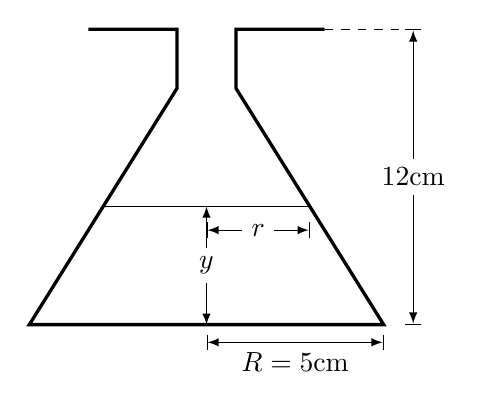
\begin{tikzpicture}[>=latex, scale=1.5]
        \draw[very thick](-1,2.5)--(-.25,2.5)--(-.25,2)--(-1.5,0)--(1.5,0)--(.25,2)--(.25,2.5)--(1,2.5);
\draw[|<->|](1.75,0)--node[fill=white]{12cm}(1.75,2.5);
\draw[dashed](1,2.5)--(1.75,2.5);
\draw[|<->|](0,-.15)--node[below]{$R=5$cm}(1.5,-.15);
\draw(-1.75/2,1)--(1.75/2,1);
\draw[<->](0,0)--node[fill=white]{$y$}(0,1);
\draw[|<->|](0,.8)--node[fill=white]{$r$}(1.75/2,.8);
    \end{tikzpicture}
    \caption{}
    \end{minipage}
    \end{figure}

\begin{example}
有一底半径为5cm, 高为12cm的正圆锥形容器(图2.10), 以每秒2$\rm cm^3$的速度往容器中倒水,试求容器水位等于锥高一半时,水面上升速度.
\end{example}


\begin{solution}
    设在某时刻$t$, 容器水高为$y$, 则此时水的体积$V$为
 \begin{align*}
     V&=\frac{\pi R^2h}{3}-\frac{\pi r^2}{3}(h-y)\\
     &=\frac{\pi}{3}\cdot 5^2\cdot 12-\frac{\pi r^2}{3}(12y)\\
     &=100\pi-\frac{\pi r^2}{3}(12-y)
 \end{align*}
而
\[\frac{r}{R}=\frac{h-y}{h}\]
即
\[r=\frac{R}{h}(h-y)=\frac{5}{12}(12-y)\]
代入上式,得
\begin{align*}
    V&=100\pi-\frac{\pi}{3}\cdot \frac{5^2}{12^2}(12-y)^3\\
    &=100\pi-\frac{25\pi}{432}(12-y)^3
\end{align*}
又由题设知:$V=2t$,所以
\[2t=100\pi-\frac{25\pi}{432}(12-y)^3\]
即
\begin{equation}
    t=50\pi-\frac{25\pi}{864}(12-y)^3
\end{equation}
这就确定了水的高度与时间$t$的关系,水面上升速度就是
$y$关于时间$t$的变化率,也就是$\frac{\dd y}{\dd t}$.根据反函数求导法则,有
\[\frac{\dd y}{\dd t}=\frac{1}{\frac{\dd t}{\dd y}}\]
由(2.8)得
\[\frac{\dd t}{\dd y}=\frac{25\pi}{864}\cdot 3(12-y)^2(12-y)'=\frac{25\pi}{288}(12-y)^2\]

$\therefore\quad \frac{\dd y}{\dd t}=\frac{288}{25\pi(12-y)^2}$

当$y=\frac{1}{2}h=6$时,
\[\left.\frac{\dd y}{\dd t}\right|_{y=6}=\frac{288}{25\x 36\pi}\approx 0.102({\rm cm/s})\]

答:水面上升速度为每秒0.102厘米.
\end{solution}

\begin{ex}
\begin{enumerate}
    \item 求下列函数的微商:
\begin{multicols}{2}
\begin{enumerate}
  \item $\arcsin \frac{x}{4}$
\item  $\arccos x^{2}$
\item  $\arctan \frac{1}{x}$
\item  $\arcsin \sqrt{x}$
\item  $(\arcsin x)^{2}$
\item  $\arctan (\tan  x)$
\item $\arctan \frac{2 x}{1-x^{2}}$
\item  $\arctan (2 \tan  x)$
\item $x^{2} \arccot \frac{x}{a}$
\item $\ln \sqrt{1+4 x^{2}} \cdot \arccot \frac{1-x}{1+x}$
\item  $\frac{1-\arccos 2 x}{\arctan x}$
\item  ${\rm arccsc}\, x$
\end{enumerate}
\end{multicols}

\item 证明
   \[
    \frac{\dd}{\dd x}\left\{\arctan \left(\frac{\sin x}{\cos 2 x}\right)\right\}=\frac{3 \cos x-\cos 3 x}{2(1-\sin x \sin 3 x)}
   \]
    \item 求下列函数的导数:
\begin{enumerate}
\item $\arcsin \cdot \frac{6 x^{2}}{\sqrt{4+81 x^{8}}}$
\item $\arctan \frac{1}{1-3 x^{2}}-\arctan \frac{1}{1+3 x^{2}}$
\item $\arccot \frac{4 \sqrt{x}}{1-4 x}$
\end{enumerate}

\item 一圆锥形容器,深10尺,上顶圆半径为4尺;求
\begin{enumerate}
    \item 灌入水时,水的体积$V$对水面高度$h$的变化率;
    \item 体积$V$对容器截面圆半径$R$的变化率.
\end{enumerate}

\item 一圆锥形容器底面朝上放着,它的顶角为$2\arctan\frac{3}{4}$, 
今向里面倒进某种液体,试求
\begin{enumerate}
\item 当液面半径$r$为3, 半径增加的速度$\frac{\dd r}{\dd t}$为$\frac{1}{4}$时,
体积增加的速度$\frac{\dd V}{\dd t}$;
\item 当液面半径为6, 体积增加的速度为24时,半径增加的速度.
\end{enumerate}

\item 水从高为18厘米,底半径为6厘米的圆锥形漏斗中流入半
径为5厘米的圆柱形筒内.已知此漏斗中水深为12厘米时,漏斗中水面的下降速度为1厘米/分,求此时圆筒中水面的上升速度.
\item 底数$a$为什么值时,直线$y=x$才能与对数曲线$y=\log_a x$相切?在何处相切?
\item 求曲线$y=e^{-x}$上的一点,使过该点的切线与直线$y=-ex$平行,并写出该点的法线方程.
\item 求曲线$y=\frac{1}{2}(1+2x^2\pm \sqrt{1+4x^2})$上横坐标$x=u$的点
处的切线方程.这切线还与曲线交于何处?$y$的反函数为何?
\end{enumerate}    
\end{ex}

\subsection{隐函数的导数}

到现在为止,我们所讨论的函数都是可以由自变量明显地表示出来的函数,例如,方程
$y=x^3+1$
就定义了一个明显的函数$f$, 这里$f(x)=x^3+1$. 这种函数叫做显函数.但是并不是所有的函数都可以用这种明显的表达式来定义的,例如由下面的$x,y$的方程
\[x^3-x=y^3-y^2+24\]
就不容易解出用$x$表示$y$的解,或用$y$表示$x$的解.但是,却有可能存在一个函数$f$, 使得方程
\[x^3-x=f^3(x)-f^2(x)+24\]
对于函数$f$的定义域中的一切$x$值都成立,这样一个函数,如果存在的话,就叫做被这个方程定义的隐函数.最简的情形是二元一次方程:
\[Ax+By+C=0\]
当$B\ne 0$时,就定义一个隐函数$f:\; \mathbb{R}\mapsto \mathbb{R}$, 这里$f(x)=-\frac{A}{B}x-\frac{C}{B}$. 

应该注意:
\begin{enumerate}
\item 方程$F(x,y)=0$的解有可能不存在,例如方程$x^2+y^2+1=0$没有实数解,因此,由它不能定义一个隐函数.
\item 由方程$F(x,y)=0$可能定义几个函数.例如,由方程
$x^2+y^2=16$
就定义了两个函数:
\[f_1 (x) =\sqrt{16-x^2},\qquad x\in [-4, 4] \]
和
\[f_2 (x) =-\sqrt{16-x^2},\qquad x\in  [-4, 4] \]
\end{enumerate}

\begin{blk}
    {定义} 方程
    \begin{equation}
 F (x,y) =0       
    \end{equation}
给出了变元$x,y$之间的一个关系.如果存在一个函数$y=
f(x)$, 或$x=g(y)$使得对于函数的定义域中的一切值,等式$F(x,f(x))=0$或$F(g(x),y)=0$恒成立,我们就说方程(2.8)定义了一个\textbf{隐函数}:
\[y=f(x)\qquad \text{或}\qquad x=g(y)\]
\end{blk}

要对方程(2.8)给出的隐函数求导数,通常的办法是直接对这个方程求导数,而不是先解出显函数,再来求导数.


\begin{example}
设$xy+x^2-1=0$,求$y'_x$.
\end{example}

\begin{solution}
先把$y$看成$x$的函数,即$y=f(x)$, 然后,在等式
$xf (x) +x^2-1=0$
的两边对$x$求导数,得到
\begin{align*}
    (x\cdot f(x))'+(x^2)'&=0\\
xf'(x)+f(x)+2x&=0
\end{align*}

$\therefore\quad f (x) =-\frac{2x+f (x)}{x}=-\frac{2x+\frac{1-x^2}{x}}{x}=-\frac{1+x^2}{x^2}$    
\end{solution}

\begin{example}
    方程$x^2+y^2=16$定义了两个可微函数:
$y=\sqrt{16-x^2}$和$y=-\sqrt{16-x^2},\; x\in [-4, 4]$. 求每一个函数的导数.
\end{example}


\begin{solution}
    我们用$f(x)$代表上面两个函数中的任何一个,则
\[x^2+f^2 (x) =16,\qquad  x\in  [-4, 4] \]
对上面等式的两边微分,得到
\begin{align*}
    2x+2f (x) \cdot f' (x) &=0\\
    f'(x)&=-\frac{x}{f(x)}
\end{align*}
即
\begin{align*}
    \left(\sqrt{16-x^2}\right)'&=-\frac{x}{\sqrt{16-x^2}}\\
    \left(-\sqrt{16-x^2}\right)'&=\frac{x}{\sqrt{16-x^2}},\qquad x\in[-4,4]
\end{align*}
\end{solution}

\begin{rmk}
应用这个方法求隐函数的导数时,我们作了两点假设:
\begin{enumerate}
    \item 存在一个由方程$F(x,y)=0$定义的函数;
    \item 这样定义的函数是可微的.
\end{enumerate} 
至于在什么条件下,这种假设是合理的问题,已经超出了本书的范围,故不在此讨论.
\end{rmk}

\begin{example}
求证椭圆$\frac{x^2}{a^2}+\frac{y^2}{b^2}=1$在点$(x_0,y_0)$处切线的方程为$\frac{x_0x}{a^2}+\frac{y_0y}{b^2}=1$.
\end{example}

\begin{proof}
\begin{align*}
    \left(\frac{x^2}{a^2}+\frac{y^2}{b^2}\right)'_x&=(1)'_x\\
    \frac{2x}{a^2}+\frac{2y}{b^2}\cdot y_x&=0
\end{align*}
若$y\ne 0$,则:
\[y'_x=-\frac{b^2x}{a^2y}\]
于是,在点$(x_0,y_0)$处(这里$y_0\ne 0$)的切线方程为
\[y-y_0=-\frac{b^2x}{a^2y}(x-x_0)\]
即:$b^2x_0x+a^2y_0y=b^2x^2_0+a^2y^2_0$

$\because\quad $点$(x_0,y_0)$在椭圆上,

$\therefore\quad b^2x_0^2+a^2y^2_0=a^2b^2$,因此,所求切线方程是
\[b^2x_0 x+a^2y_0 y=a^2b^2\]
也就是
\[\frac{x_0x}{a^2}+\frac{y_0y}{b^2}=1\]

若$y=0$则$x=\pm a$, 显然在点$(-a,0)$和点$(a,0)$处的切线方程分别是$x=-a$, $x=a$, 它们是方程$\frac{x_0x}{a^2}+\frac{y_0y}{b^2}=1$的特殊形式.
\end{proof}
    
\begin{example}
    如果将抛物线$y^2=2px$绕它的对称轴旋转成旋转挑物面,那么与对称轴平行的光线射到曲面上,经曲面反射后通过焦点,试证明之.
\end{example}


\begin{proof}
从物理学知道,光线经镜面反射后,要服从光的反射定律:
\begin{enumerate}
    \item 在均匀介质中,光沿直线传播.
    \item 当光线碰到平面镜时,光线要反射.入射线与镜面法线夹角(记作$i$)等于反射线与镜面法线的夹角(记作$r$),见图2.11, 角$i$称为入射角,角$r$称为反射角.
\item 光从曲面镜的反射也遵守同样的法则:
  \[  \text{入射角}i=\text{反射角}r\]
    此时镜面的法线定义为与镜面在入射点的切线相垂直的直线.
\end{enumerate}

\begin{figure}[htp]
    \centering
    \begin{tikzpicture}[>=latex, scale=1]
        \fill[pattern=north east lines](-2,-.25) rectangle (2,0);
        \draw(-2,0)node[left]{镜面}--(2,0);
        \draw[->, very thick](140:3)node[left]{入射线}--(140:2);
        \draw[->, very thick](140:2)--(0,0)--(40:3)node[right]{反射线};
        \draw(0,0)--(0,3)node[above]{法线};
        \draw[<->, thick](90:1.8) arc (90:40:1.8);
        \draw[<->, thick](90:1.8) arc (90:140:1.8);
        \node at (60:2){$r$};
        \node at (120:2){$i$};
            \end{tikzpicture}
    \caption{}
\end{figure}

假设光线经位于$xy$平面上的抛物线$y^2=2px$形的镜面反射.当入射线与x轴平行且与抛物线交于$P_1(x_1,y_1)$点时,我们要求反射线的方
程,并证明它通过焦点$F\left(\frac{p}{2},0\right)$. 如果过$P_1(x_1,y_1)$点的切线与$x$轴成$\theta$角,那么平行于$x$轴的入射光线与法线的夹角是$90^{\circ}-\theta$. 由光的反射定律,反射光线与法线的夹角也是$90^{\circ}-\theta$. 于是,从图2.12上看出,反射光线与$x$轴的夹角是$2\theta$.

现在,在方程$y^2=2px$的两边对$x$求导数,得到
\[2yy'=2p\quad \Rightarrow\quad y'=\frac{2p}{2y}=\frac{p}{y}\]
所以,由导数的几何意义得出,在$P_1(x_1,y_1)$点的切线的斜率是
\[\tan\theta=y'_{x_1}=\frac{p}{y_1}\]
于是反射光线的斜率是
\begin{align*}
    \tan2\theta=\frac{2\tan\theta}{1-\tan^2\theta}&=\frac{2\cdot \frac{p}{y_1}}{1-\frac{p^2}{y^2_1}}\\
    &=\frac{2py_1}{y^2_1-p^2}=\frac{2py_1}{2px_1-p^2}=\frac{2y_1}{2x_1-p}
\end{align*}
从而,得出反射线方程
\[y-y_1=\frac{2y_1}{2x_1-p}(x-x_1) \]
令$y=0$, 得到反射光线与$x$轴交点的横坐标,
\[0-y_1=\frac{2y_1}{2x_1-p}(x-x_1)\quad \Rightarrow\quad x=\frac{p}{2}\]
即反射线通过焦点$F\left(\frac{p}{2},0\right)$. 由于$P_1(x_1,y_1)$是抛物线上
任意一点,所以只要入射光线与$x$轴平行,反射光线必通过焦
点.如果把光源放在焦点$F\left(\frac{p}{2},0\right)$上,那么从焦点发出的
光线经抛物线镜面反射后的反射光线是与对称轴($x$轴)平行的光线.我们常利用这个原理获得平行光.
\end{proof}

\begin{figure}[htp]\centering
\begin{tikzpicture}[>=latex, scale=1.2]
\draw[->](-1.5,0)--(5,0)node[right]{$x$};
\draw[->](0,-3)--(0,3)node[right]{$y$};
\draw[domain=2.5:-2.5, samples=100, very thick]plot({0.5*\x*\x}, \x)node[right]{$y^2=2px$};
\draw[domain=-1:3.5, samples=10, thick]plot(\x, {0.707*(\x+1)});
\draw[thick](.5,0)node[below right]{$F\left(\frac{p}{2},0\right)$}--(1,1.414)--(4,1.414);
\draw[->, thick](4,1.414)--(3,1.414);
\tkzDefPoints{-1/0/A, 1/1.414/P, .5/0/F, 4/1.414/B, 3/2.828/C, 5/0/D}
\tkzMarkAngles[mark=none, size=.45](D,A,P D,F,P A,P,F B,P,C)
\tkzLabelAngle[pos=.6](D,A,P){$\theta$}
\tkzLabelAngle[pos=.6](D,F,P){$2\theta$}
\tkzLabelAngle[pos=.6](A,P,F){$\theta$}
\tkzLabelAngle[pos=.6](B,P,C){$\theta$}

\draw[domain=.5:1.5, samples=10]plot(\x, {1.414*(-\x+2)});
\tkzDefPoints{1.5/0.707/E}
\tkzMarkAngles[mark=none, size=.6, <->](E,P,B)
\tkzLabelAngle[pos=1.2](E,P,B){$90^{\circ}-\theta$}
\node at (P) [left]{$P_1(x_1,y_1)$};
\node at (0,0)[below left]{$O$};
\end{tikzpicture}
\caption{}
\end{figure}

\begin{ex}
\begin{enumerate}
    \item 求下列隐函数在指定点的导数$\frac{\dd y}{\dd x}$:
\begin{enumerate}
    \item $y=\cos x+\frac{1}{2}\sin y$, 点$\left(\frac{\pi}{2},0\right)$
    \item $ye^x+\ln y=1$, 点$\left(0,1\right)$
    \item $x^2+xy+y^2=1$, 点$\left(1,-1\right)$
    \item $x^2y^2+x^2+y^2=9$, 点$\left(1,2\right)$
\end{enumerate}
    \item 求下列隐函数的导数$\frac{\dd y}{\dd x}$:
\begin{multicols}{2}
\begin{enumerate}
    \item $\frac{x^2}{a^2}+\frac{y^2}{b^2}=1$
    \item $y^2=8x$
    \item $x^2=2y$
    \item $\sqrt{x}+\sqrt{y}=1$
    \item $x^3+y^3=a^3$
    \item $x^{\tfrac{2}{3}}+y^{\tfrac{2}{3}}=a^{\tfrac{2}{3}}$
    \item $y-\cos(x+y)=0$
    \item $y=x+\arctan y$
    \item $y=1-\ln(x+y)+e^y$
    \item $\arctan \frac{y}{x}=\ln\sqrt{x^2+y^2}$
\end{enumerate}
\end{multicols}

\item 求下列方程在指定点的导数$\frac{\dd y}{\dd x}$:
\begin{enumerate}
    \item $x-\sqrt{xy}+y=2$,点$(x_1,y_1)$
    \item $(ax)^{\tfrac{2}{3}}-(by)^{\tfrac{2}{3}}=(a^2+b^2)^{\tfrac{2}{3}}$,点$(x_0,y_0)$
    \item $(x+y)^{\tfrac{2}{3}}+(x-y)^{\tfrac{2}{3}}=2a^{\tfrac{2}{3}}$在$x=0$的点;在$x=y$的点;在$x=-y$的点
    \item $x^2+xy+y^2=c^2$,在斜率等于$-1$的点
\end{enumerate}
\item 若$x\sqrt{y}+y\sqrt{x}=c$,求$\frac{\dd y}{\dd x}$和$\frac{\dd x}{\dd y}$.
\item 求椭圆$x^2+4y^2=9$的切线方程,使它和直线$2x+3y=0$
平行.
\item 曲线$y=(x-2)(x-3)(x-4)$和$x$轴交于$P(2, 0)$, $Q(3,0)$和$R(4, 0)$点.
\begin{enumerate}
    \item 求证在$P$点和$R$点处的切线互相平行;
    \item 求曲线在$Q$点处的法线与$y$轴的交点.
\end{enumerate}
\item 求曲线 $2x^3-xy+8=0$上的$P$点,使在该点的切线通过
原点,过$P$点的切线与曲线交于另一点$Q$的坐标.
\item \begin{enumerate}
    \item 求证直线$\ell x +my+n=0$与椭圆$\frac{x^2}{a^2}+\frac{y^2}{b^2}=1$, 双曲线$\frac{x^2}{a^2}-\frac{y^2}{b^2}=1$, 抛物线$y^2=2px$相切的条件分别是$a^2\ell^2+b^2m^2=n^2$, $a^2\ell^2-b^2m^2=n^2$, $pm^2=2n\ell$.
    \item 证明对于任意$k$, 直线$y=kx+\sqrt{a^2k^2+b^2}$是椭圆曲线$\frac{x^2}{a^2}+\frac{y^2}{b^2}=1$的切线.    
\end{enumerate}
\item \begin{enumerate}
    \item 求过$P(5, 3)$点与椭圆$\frac{x^2}{16}+{y^2}=1$相切的直线
    方程.
    \item 求过(a)中的两切点的直线方程.
\end{enumerate}

\item 椭圆$\frac{x^2}{16}+{y^2}=1$的切线与$x$轴成$60^{\circ}$角,求该切线的方程.
\item 通过双曲线$\frac{x^2}{a^2}-\frac{y^2}{b^2}=1$的焦点而与横轴垂直的弦的
两个端点分别记作$A$和$B$, 求证过$A$、$B$两点的切线交于
横轴上的点$Q$, 且$Q$点离中心的距离等于$\frac{a}{e}$.
\item 求证过双曲线上一点$P$的切线与过$P$点的焦点半径成等角.
\end{enumerate}
\end{ex}

\subsection{高阶导数}
对于给定的可微函数$f(x)$, 它的导数$f'(x)$仍是$x$的函数.如果$f'(x)$是可微的,它的导函数$(f'(x))'=f''(x)$或$f^{(2)}(x)$称为$f(x)$的\textbf{二阶导函数},……如此类推,$f(x)$
的$n$阶导函数$f^{(n)}(x)$, 可以归纳地定义为:
\begin{align*}
  f ^{(1)} (x)&=f'(x)\\
  f ^{(n)} (x)&=\left(f^{(n-1)}(x)\right)',\qquad n=2,3,\ldots  
\end{align*}
因此,求高阶导函数,实际上就是连续地求一阶导函数.

高阶导函数有时也记作$\frac{\dd^n y}{\dd x^n}$或$\frac{\dd^n }{\dd x^n}f(x)$. 例如
\begin{align*}
    f''(x)&=\frac{\dd}{\dd x}f'(x)=\frac{\dd}{\dd x}\left(\frac{\dd y}{\dd x}\right)=\frac{\dd^2 y}{\dd x^2}\\
    f^{(3)}(x)&=\frac{\dd}{\dd x}\left(\frac{\dd^2 y}{\dd x^2}\right)=\frac{\dd^3 y}{\dd x^3}
\end{align*}

二阶导数有它的实际意义,例如动点的速度$v$等于它所
经过的路程$S$对于时间$t$的变率:$v=\frac{\dd S}{\dd t}$;而加速度$a$是速度$v$
对于时间$t$的变率:$a=\frac{\dd v}{\dd t}$,
这就是说加速度是路程$S$对于时间$t$的二阶导数:$a=\frac{\dd^2 S}{\dd t^2}$.
在以后的学习中,我们还会知道二阶导数有它的重要的几何意义.我们已经知道一次函数$f(x)=ax+b\; (a\ne 0)$的图象是一条直线,而它的二阶导数$f''(x)=(f'(x))'=(a)'=0$. 因此,若一函数的二阶导数$f''(x)\ne 0$, 那么它的图象就不是直线.

\begin{example}
设$y=\frac{x}{1-x}$,求$\frac{\dd^2 y}{\dd x^2}$, $\frac{\dd^3 y}{\dd x^3}$.
\end{example}

\begin{solution}
\begin{align*}
    y&=\frac{x}{1-x}=-1+\frac{1}{1-x}\\
\frac{\dd y}{\dd x}&=-\frac{(1-x)'}{(1-x)^2}=\frac{1}{(1-x)^2}
\end{align*}
\begin{align*}
    \frac{\dd^2 y}{\dd x^2}&=\frac{-[(1-x)^2]'}{(1-x)^4}=\frac{-2(1-x)(-1)}{(1-x)^4}=\frac{2}{(1-x)^3}\\
    \frac{\dd^3 y}{\dd x^3}&=\frac{-2[(1-x)^3]'}{(1-x)^6}=\frac{2\cdot 3(1-x)^2(-1)}{(1-x)^6}=\frac{6}{(1-x)^4}  
\end{align*}
\end{solution}


\begin{example}
若$f(x)=\sqrt{a^2+x^2}$,求$f''(x)$
\end{example}


\begin{solution}
\textbf{解法1: }
\begin{align*}
    f'(x)&=\frac{1}{2}(a^2+x^2)^{-\tfrac{1}{2}}(a^2+x^2)'\\
    &=\frac{1}{2}(a^2+x^2)^{-\tfrac{1}{2}}(2x)=\frac{x}{\sqrt{a^2+x^2}}\\
\end{align*}
\begin{align*}
f''(x)&=\frac{\sqrt{a^2+x^2}\cdot x'-x\left(\sqrt{a^2+x^2}\right)'}{a^2+x^2}\\
&=\frac{\sqrt{a^2+x^2}-\frac{x^2}{\sqrt{a^2+x^2}}}{{a^2+x^2}}\\
&=\frac{a^2+x^2-x^2}{(a^2+x^2)^{\tfrac{3}{2}}}=\frac{a^2}{(a^2+x^2)^{\tfrac{3}{2}}}
\end{align*}

\textbf{解法2: } 将原来的函数变形为隐函数,用隐函数微分法求二阶导数.

设$y=\sqrt{a^2+x^2}$, 则$y^2=a^2+x^2$, 对$x$微分得:
\[y\cdot y_x=x\]    
再对$x$微分得:
\[y\cdot y_x''+(y_x')^2=1\]
将$y'=\frac{x}{y}$代入,得
\[y\cdot y''_x+\frac{x^2}{y^2}=1\]
因此:
\[y''_x=\frac{1-\frac{x^2}{y^2}}{y}=\frac{1-\frac{x^2}{x^2+a^2}}{\sqrt{a^2+x^2}}=\frac{a^2}{(a^2+x^2)^{\tfrac{3}{2}}}\]
\end{solution}

\begin{example}
    若$y=\frac{x^2}{\sqrt{x^2+1}}$,求证:
\[(x^2+1)\frac{\dd^2 y}{\dd x^2}+3x\frac{\dd y}{\dd x}-y=2\sqrt{x^2+1}\]
\end{example}

\begin{proof}
将原式去分母
\[y\sqrt{x^2+1}=x^2\]
对$x$微分得
\[\sqrt{x^2+1}\cdot\frac{\dd y}{\dd x}+y\cdot \frac{x}{\sqrt{x^2+1}}=2x\]
两边乘以$\sqrt{x^2+1}$,得到
\[(x^2+1)\cdot \frac{\dd y}{\dd x}+y\cdot x=2x\sqrt{x^2+1}\]
再对$x$微分得:
\[(x^2+1)\frac{\dd^2 y}{\dd x^2}+(2x)\cdot \frac{\dd y}{\dd x}+x\frac{\dd y}{\dd x}+y=2\sqrt{x^2+1}+\frac{2x^2}{\sqrt{x^2+1}}\]
即:
\[(x^2+1)\frac{\dd^2 y}{\dd x^2}+3x\frac{\dd y}{\dd x}+y=2\sqrt{x^2+1}+2y\]
因此:
\[(x^2+1)\frac{\dd^2 y}{\dd x^2}+3x\frac{\dd y}{\dd x}-y=2\sqrt{x^2+1}\]
\end{proof}

有时需要求一些函数的$n$阶导数,但是在一般情形下,函数的$n$阶导数是如此的复杂,以致求函数的$n$阶导数的通式是办不到的,然而有一些函数,我们不难写出它的$n$阶导数的通式.

\begin{example}
  设$y=(ax+b)^m$, 求$y^{(n)}\; (m>n)$  
\end{example}

\begin{solution}
\begin{align*}
y'&=ma(ax+b)^{m-1}\\
y''&=m(m-1)a^2(ax+b)^{m-2}\\
y^{(3)}&=m(m-1)(m-2)a^3(ax+b)^{m-3}\\
\cdots\quad &\cdots\quad \cdots
\end{align*}
由此推知:
\[y^{(n)}=m(m-1)\cdots(m-n+1)a^n(ax+b)^{m-n}=\frac{m!}{(m-n)!}a^n(ax+b)^{m-n}\]
这个结果的正确性可用数学归纳法证明.
\end{solution}


\begin{example}
设$y=\frac{1}{x^2-4x+3}$,求$y^{(n)}$.
\end{example}


\begin{solution}
\[y=\frac{1}{x^2-4x+3}=\frac{1}{2}\left(\frac{1}{x-3}-\frac{1}{x-1}\right)\]
\begin{align*}
    y'&=\frac{1}{2}\left[\frac{-1}{(x-3)^2}-\frac{-1}{(x-1)^2}\right]=\frac{(-1)}{2}\left[\frac{1}{(x-3)^2}-\frac{1}{(x-1)^2}\right]\\
    y''&=\frac{(-1)}{2}\left[\frac{-2(x-3)}{(x-3)^4}-\frac{-2(x-1)}{(x-1)^4}\right]=\frac{(-1)^2 2!}{2}\left[\frac{1}{(x-3)^3}-\frac{1}{(x-1)^3}\right]\\
    \cdots\quad &\cdots\quad \cdots
\end{align*}
假设一般地有:
\[y^{(n)}=\frac{(-1)^n n!}{2}\left[\frac{1}{(x-3)^{n+1}}-\frac{1}{(x-1)^{n+1}}\right]\]
那么:
\begin{align*}
    y^{(n+1)}&=\frac{(-1)^n n!}{2}\left[\frac{-(n+1)(x-3)^n}{(x-3)^{2(n+1)}}-\frac{-(n+1)(x-1)^n}{(n-1)^{2(n+1)}}\right]\\
    &=\frac{(-1)^{n+1} (n+1)!}{2}\left[\frac{1}{(x-3)^{n+2}}-\frac{1}{(x-1)^{n+2}}\right]
\end{align*}
即仍有此规律.因此,对于任何自然数$n$,都有
\[y^{(n)}=\frac{(-1)^n n!}{2}\left[\frac{1}{(x-3)^{n+1}}-\frac{1}{(x-1)^{n+1}}\right]\]
成立.
\end{solution}

\begin{example}
    设$y=\sin(ax+b)$,求$y^{(n)}$.
\end{example}


\begin{solution}
    \[y'=a\cos(ax+b)=a\sin\left(ax+b+\frac{\pi}{2}\right)\]
因此,求$\sin(ax+b)$的导数是将函数乘以$a$,同时将幅角加上$\frac{\pi}{2}$.

不难推知:
\[y^{(n)}=a^n\sin\left(ax+b+\frac{n\pi}{2}\right)\]
请读者用数学归纳法证明这个猜想正确.
\end{solution}

\begin{example}
设$f(x)=a_0+a_1x+a_2x^2+\cdots+a_nx^n$,$h$为任取非零实数,求证:
\[f(a+h)=f(a)+f'(a)h+\frac{f''(a)}{2!}h^2+\cdots+\frac{f^{(n)}(a)}{n!}h^n\]
\end{example}


\begin{proof}
已给$f(x)=a_0+a_1x+\cdots+a_nx^n$,令$x=a+h$,并按$h$的升幂展开每一项,得到一个形式如
\begin{equation}
    f(a+h)=C_0+C_1 h+C_2 h^2+\cdots +C_n h^n
\end{equation}
的表达式.

我们将说明,系数$C_0,C_1,\ldots,C_n$由$f(x)$在点$a$的函数值$f(a)$以及直到$n$阶为止的各阶导数在$x=a$的值表示,即
\[C_0=f (a) ,\quad  C_i =\frac{1}{i!}f' (a) ,\qquad i=1, 2,\ldots ,n\]

为了证明这个事实,(2.10)中把$h$看作自变量,首先令$h\to 0$, 立刻得到
\[f (a) =C_0\]

然后,应用复合函数求导法则,对方程(2.10), 关于$h$逐次求导,依次得到:
\begin{align*}
f'(a+h)&=C_1+2C_2 h+3C_3h^2+\cdots +nC_nh^{n-1}\\
f''(a+h)&=2C_2+3\x 2C_3h+\cdots+n(n-1)C_nh^{n-2}\\
f^{(3)}(a+h)&=3!C_3+\frac{4!}{1!}C_4h+\frac{5!}{2!}C_5x^2+\cdots+\frac{n!}{(n-3)!}C_nh^{n-3}\\
\cdots\quad &\cdots\quad \cdots\\
f^{(i)}(a+h)&=i! C_i+\frac{(i+1)!}{1!}C_{i+1}h+\cdots+\frac{n!}{(n-i)!}C_nh^{n-i}\\
\cdots\quad &\cdots\quad \cdots\\
f^{(n-1)}(a+h)&=(n-1)!C_{n-1}+n!C_nh\\
f^{(n)}(a+h)&=n!C_n
\end{align*}
把$h=0$代入上面一个方程中,便得到
\[C_1=f^{(1)}(a),C_2=\frac{f^{(2)}(a)}{2!},C_3=\frac{f^{(3)}(a)}{3!},\ldots,C_i=\frac{f^{(i)}(a)}{i!},\ldots,C_n=\frac{f^{(n)}(a)}{n!}\]

把上面$C_0=f(a),\; C_i=\frac{f^{(i)}(a)}{i!},\quad i=1,2,\ldots,n$代入(2.10)中,最后得到:
\begin{equation}
    f(a+h)=f(a)+f'(a)h+\frac{f^{(2)}(a)}{2!}h^2+\cdots+\frac{f^{(n)}(a)}{n!}h^n
\end{equation}
这个公式叫做多项式的泰勒公式.

在(2.11)中,令$a+h=x$, 则(2.11)可以改写成
\[    f(x)=f(a)+f'(a)(x-a)+\frac{f^{(2)}(a)}{2!}(x-a)^2+\cdots+\frac{f^{(n)}(a)}{n!}(x-a)^n\]
\end{proof}

\begin{ex}
\begin{enumerate}
    \item 求下列函数的$n$阶导数:
\begin{multicols}{2}
\begin{enumerate}
    \item $f(x)=\frac{1-x}{1+x}$
    \item $f(x)=\sin^2 x$
\end{enumerate}
\end{multicols}
    \item 若$y=\tan(m\cdot \arctan x)$,验证
\[(1+x^2)\frac{\dd^2 y}{\dd x^2}=2(my-x)\frac{\dd y}{\dd x}\]
\item 若$y=\frac{A\cos mx+B\sin mx}{x^n}$,其中$A,B,m,n$是常数,验证
\[\frac{\dd^2 y}{\dd x^2}+2\frac{n}{x}\frac{\dd y}{\dd x}+\left[\frac{n(n-1)}{x^2}+m^2\right]y=0\]

\item 若$h(x)=f(x)g(x)$,其中$f(x)$, $g(x)$和$h(x)$都是$n$阶可微,求证:
\begin{align*}
    h^{(n)}(x)&=f(x)\cdot g^{(n)}(x)+C^1_n f^{(1)}(x)g^{(n-1)}(x)+\cdots \\
    &\qquad +C^h_n f^{(h)}(x)g^{(n-h)}(x)+\cdots\\
    &\qquad  +C^{n-1}_n f^{(n-1)}(x)g^{(1)}(x)+C^n_n f^{(n)}(x)g(x)
\end{align*}
\item 求下列函数的$n$阶导数:
\begin{multicols}{2}
\begin{enumerate}
\item $f(x)=x\ln x$
\item $f(x)=xe^x$
\item $f(x)=e^{ax}\sin\beta x$
\end{enumerate}
\end{multicols}
\item 证明 $x^3-7x^2+15x-9=0$有一个二重根.
\item 检验方程 $x^3-6x^2+11x-6=0$有无重根?
\item 方程$x^4-6x^2-8x-3=0$有重根,解此方程.
\item 应用泰勒公式将多项式$(x+a)^n$按$x$的升幂展开.
\item 若$f(x)=x^3-3kx+2k+8$在实数范围内能分解成一个二重因式,试求$k$值和它的因式乘积.
\end{enumerate}   
\end{ex}

\subsection{参数方程表示的函数的导数}
用方程$y=f(x)$来表示曲线在几何上受很大的限制:这样表示的曲线与平行于$y$轴的任意直线相交不能多于一点.通常,把曲线分成可以表为$y=f(x)$的若干部分来克服这个限制,例如,以原点为中心,$r$为半径的圆,可以由定义在闭区间$[-r,r]$上的两个函数$y=\sqrt{r^2-x^2}$和$y=-\sqrt{r^2-x^2}$给出.

曲线最直接和最灵活的描述法是参数表示.我们不把直角坐标$x$或$y$中的一个看成另一个的函数,而把两个坐标$x$和$y$都看成为第三个自变量$t$的函数,$t$叫做\textbf{参数}或\textbf{参变量}.当$t$在$t$轴上或$t$轴上的一个区间$[a,b]$变化时,由$t$轴上的原象点,通过参数方程$x=\varphi(t)$, $y=\psi(t)$映射到曲线$C$上的一点$(x,y)=(\varphi(t),\psi(t))$, 使得对应于$t$的某个区间$[a,b]$或$(-\infty, \infty)$, 一对函数值$x=\varphi(t)$, $y=\psi(t)$定义的点集
$$\Big\{\big(\varphi(t), \psi(t)\big)\Big|t\in [a,b]\Big\}$$
就是曲线$C$上的全部点,而且没有其它点.

在解析几何中,我们已经知道:

圆的参数方程是
\[x=a\cos t,\qquad y=a\sin t\]
这里$t$表示圆心角.

椭圆的参数方程是
\[x=a\cos t,\qquad y=b\sin t\quad (a>b>0)\]
这里$t$是偏心角.(图2.13)

\begin{figure}[htp]
    \centering
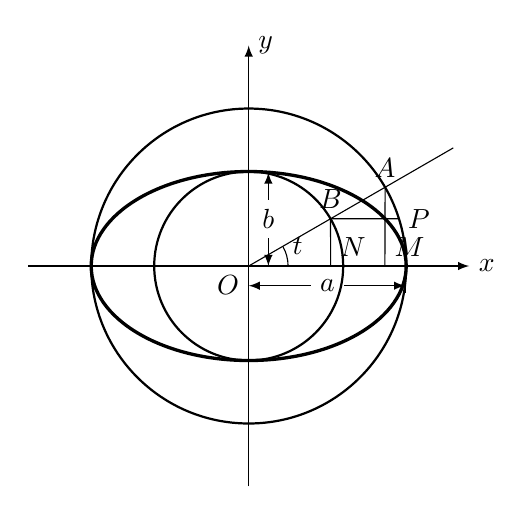
\begin{tikzpicture}[>=latex]
    \draw[<->|](0,-.25)--node[fill=white]{$a$}(2,-.25);
    \draw[<->|](.25,0)--node[fill=white]{$b$}(.25,1.2);
\draw[->](-2.8,0)--(2.8,0)node[right]{$x$};
\draw[->](0,-2.8)--(0,2.8)node[right]{$y$};
\draw[thick](0,0) circle (2);
\draw[thick](0,0) circle (1.2);
\draw[very thick](0,0) ellipse [x radius=2, y radius=1.2];
\node at (0,0)[below left]{$O$};
\draw(0,0)--(30:3);
\draw(30:1.2)node[above]{$B$}--(1.04,0)node[above right]{$N$};
\draw(30:2)node[above]{$A$}--(1.73,0)node[above right]{$M$};
\draw(.5,0) arc (0:30:.5)node[right]{$t$};
\draw(30:1.2)--(1.9,.6)node[right]{$P$};

\end{tikzpicture}
    \caption{}
\end{figure}

曲线$C$可以有许多参数表示法,就好象同一条路可以有许多不同走法,例如抛物线$y^2=2px$可以用在其上的点$(x,y)$的切线的斜率作参数,由于
$2yy'=2p$, 所以抛物线$y^2=2px$的参数方程是
\[x=\frac{p}{2(y')^2},\qquad y=\frac{p}{y'}\]
其中$y'\in (-\infty,0)\cup (0, \infty)$.

如果用$\frac{1}{y'}=\cot\theta$作参数,那么它的参数方程是
\[x=\frac{p}{2}\cot^2 \theta,\qquad y=p\cot\theta\]

我们也可以用$\frac{y}{2p}=\frac{x}{y}=\lambda,\quad \lambda\in (-\infty, \infty)$作参数,于
是又得一参数方程
\[x=2p\lambda^2,\qquad y=2p\lambda\]


\begin{example}
讨论由参数方程
\[x=\sin t,\qquad y=\cos^2 t,\quad t\in[0,2\pi]\]
所定义的曲线$C$.
\end{example}

\begin{solution}
因为$\sin^2 t+\cos^2 t=1 $,所以曲线$C$在抛物线
\begin{equation}
    x^2+y=1
\end{equation}
上.反过来,抛物线(2.12)并不与曲线$C$一致,我们要说明限制在长方形区域$R=\{-1\le x\le 1,\; 0\le y\le 1\}$内的抛物线(2.12)上的部分是曲线$C$(图2.14).

\begin{figure}[htp]
    \centering
\begin{tikzpicture}[>=latex, scale=1.5]
    \draw[->](-2,0)--(2,0)node[right]{$x$};
    \draw[->](0,-1.5)--(0,2)node[right]{$y$};
\node at (0,0)[below left]{$O$};
\draw(-1,0) rectangle (1,1);
\draw[domain=-1.5:1.5, samples=100, very thick, dashed]plot(\x, {1-\x*\x});
\draw[domain=-1:1, samples=100, very thick]plot(\x, {1-\x*\x});
\node at (-1,0)[below left]{$(-1,0)$};
\node at (1,0)[below right]{$(1,0)$};
\node at (0,1)[above right]{$(0,1)$};
\end{tikzpicture}
    \caption{}
\end{figure}

事实上,$x=\sin t$在闭区间$[0,2\pi]$上处处连续,且在闭区间$\left[\frac{\pi}{2},\frac{3\pi}{2}\right]$上由1单调递减到$-1$,因此根据反函数存在定理,对于每一个$x\in[-1,1]$,存在唯一的一个$t$,使得$\sin t=x$成立,从而得到
\[y=1-x^2=1-\sin^2 t=\cos^2 t\in [0,1]\]
这就说明了,点$(x,1-x^2)\; (x\in [-1, 1])$在曲线$C$上,而且只有这些点在曲线$C$上,换言之,在(2.12)上的除去这些点的其它任何一点不在曲线$C$上.
\end{solution}

在参数方程$x=\varphi(t)$, $y=\psi(t)$中,由于$t$轴是有序的,我们可以用明显的方式把曲线$C$的点规定一个次序或“指向”,即如果$t_1<t_2$,那么由$t_1$映射的点在由$t_2$映射的点的前面.例如例2.38的曲线上的动点$P$随着$t$增加的方向这样运动:$P$点在$t=0$时,由点$(0,1)$开始移动到在$t=\frac{\pi}{2}$时的$(1,0)$点,然后沿原路线返回移动到$t=\pi$时的$(0,1)$点,再继续移动到在$t=\frac{3\pi}{2}$时的$(-1, 0)$点,最后又返回到在$t=2\pi$时的$(0, 1)$点.

如果函数$\varphi(t)$, $\psi(t)$的定义域是$t$轴上的闭区间$[a,b]$, 而且在这区间上的$t$的不同值对应曲线$C$上不同的点,
那么我们称$C$为\textbf{简单弧},例2.38中的抛物线,由上面知道不是简单弧,而抛物线$x=t$, $y=t^2,\; t\in [0, 1]$是简单弧的一个例子.

如果曲线$C$上的始点$P(\varphi(a),\psi(a))$与终点$P(\varphi(b),\psi(b))$相同,并且除$t=a$和$t=b$外,在$[a,b]$上没有另外一对不同值对应曲线上同一点,那么曲线$C$叫做\textbf{简单闭曲线}.$x=a\cos t$, $y=a\sin t,\; t\in [-\pi,\pi]$就是简单的闭曲线.

有时我们使用$y=f(x)$表示曲线$C$或$C$的一部分是方便的,如果$C$用参数方程$x=\varphi(t)$, $y=\psi(t)$给出,而对于曲线的一部分$t_2\le t\le t_1$, 函数$\varphi(t),\psi(t)$中的一个,譬如说$x=\varphi(t)$是单调的和连续的,那么这样的表示法总是可能的,办法是先由$x=\varphi(t)$解出它的反函数$t=\varphi^{-1}(x)$, 再代入$y=\psi(t)$中,便得到
\[y=\psi\left(\varphi^{-1}(t)\right)=f(x)\]
即$y=f(x)$是由$y=\psi(t)$和$t=\varphi^{-1}(x)$复合而成的复合函数.

要求曲线$C$的斜率,我们不必重新建立$y$对$x$的函数关系$y=f(x)$, 再去求导,只须由方程组
\begin{equation}
    \begin{cases}
        x=\varphi(t)\\ y=\psi(t)
    \end{cases}
\end{equation}
当$\frac{\dd\varphi}{\dd t}\ne 0$时,按照复合函数求导法则可以直接得到$f'(x)$.

事实上,当$\varphi'(t)\ne 0$时,$t=\varphi^{-1}(x)$的导数存在,并且是$\frac{\dd t}{\dd 
x}=\frac{1}{\varphi'(t)}$.

按照复合函数求导法则,得到
\[f'(x)=\frac{\dd y}{\dd t}\cdot \frac{\dd t}{\dd x}=\frac{\psi'(t)}{\varphi'(t)}\]
于是,当$\frac{\dd\varphi}{\dd t}\ne 0$时,就得到曲线$C$的斜率:
\begin{equation}
    \frac{\dd y}{\dd x}=\frac{\psi'(t)}{\varphi'(t)}
\end{equation}
当$\frac{\dd\psi}{\dd t}\ne 0$时,就得到
\begin{equation}
    \frac{\dd x}{\dd y}=\frac{\varphi'(t)}{\psi'(t)}
\end{equation}
因此,只要$[\varphi'(t)]^2+[\psi'(t)]^2\ne 0$, 切线总是存在的:如果$\psi'(t)=0$, 切线是水平的;如果$\varphi'(t)=0$, 切线是垂直的.

当曲线由参数方程组(2.13)给出,那么曲线上点$(x_0,y_0)$处的切线方程为
\begin{equation}
    (y-y_0)\frac{\dd x}{\dd t}-(x-x_0)\frac{\dd y}{\dd t}=0
\end{equation}

法线的斜率是$-\frac{1}{y'_x}$,因此法线方程为
\begin{equation}
    (x-x_0)\frac{\dd x}{\dd t}+(y-y_0)\frac{\dd y}{\dd t}=0
\end{equation}

\begin{example}
求椭圆$\begin{cases}
    x=a\cos t\\ y=b\sin t
\end{cases}$在点$t$的切线方程和法线方程.
\end{example}



\begin{solution}
椭圆在点t的切线方程,按照(2.16)得到
\[(y-b\sin t) (-a\sin t )-(x-a\cos t)(b\cos t)=0\]
    化简得
 \[   y ( - a\sin t) - x(b\cos t)+ab=0\]
    两边除以$-ab$, 得到在点$t$的切线方程
\[\frac{x}{a}\cos t+\frac{y}{b}\sin t=1\]

在点$t$的法线方程,按照(2.17)得到
\[(x-a\cos t) (-a\sin t)+(y-b\sin t)(b\cos t)=0\]
    化简得
\[   -ax\sin t+by\cos t+ (a^2-b^2) \sin t\cdot \cos t=0\]
    或
    \[xa\sin t-yb\cos t-\frac{c^2}{2}\sin 2t=0\]
\end{solution}    

\begin{example}
    求曲线$\begin{cases}
        x=t^2\\y=t^3
    \end{cases}$
    在点$t$的切线方程,并求此切线与曲线的另一交点的坐标.
\end{example}

\begin{solution}
在点$t$的切线方程是
\[(y-t^3)(2t)-(x-t^2)(3t^2)=0\]

若$t\ne 0$, 则得切线方程
  \[  2y-3tx+t^3=0\]
    设此切线与曲线交于$(T^2,T^3)$点,于是数$T$满足等式
   \[ 2T^3-3tT^2+t^3=0\]
    这是$T$的三次方程,它表示切线与曲线相交于三个点,由于切点的$t$值是它的二重根,根据根和系数的关系,得
\[2t+T=-(-3t)\quad \Rightarrow\quad T=-\frac{1}{2}t\]
故切线与曲线的另一交点的坐标是$\left(\frac{1}{4}t^2,-\frac{1}{6}t^3\right)$

如果再假定$\varphi''(t)$,$\psi''(t)$存在,则$y$对$x$的二阶导数可按照复合函数求导法及商的导数法来求:
\begin{align*}
    y''=\frac{\dd y'}{\dd x}&=\frac{\dd y'}{\dd t}\cdot \frac{\dd t}{\dd x}\\
    &=\frac{\dd }{\dd t}\left(\frac{\psi'(t)}{\varphi'(t)}\right)\cdot \frac{1}{\varphi'(t)}\\
    &=\frac{\varphi'(t)\psi''(t)-\psi'(t)\varphi''(t)}{\big\{\varphi'(t)\big\}^3}
\end{align*}
\end{solution}

\begin{ex}
\begin{enumerate}
    \item 设$x=\frac{1}{2}p\lambda^2$, $y=p\lambda$是抛物线以$\lambda$为参数的方程,求在
    点$\lambda$的切线方程和法线方程.
    \item 过点$(x_0,y_0)$作抛物线$y^2=2px$的两条切线,设切点的参数为$\lambda_1$和$\lambda_2$, 求证
    \[\begin{cases}
        p(\lambda_1+\lambda_2)=2y_0\\
        p_1\lambda_1\lambda_2=2x_0
    \end{cases}\]
    \item 过抛物线$y^2=2px$的定长为$c$的弦的两端作切线,求切线交点的轨迹方程.
    
    \item 求曲线
    $\begin{cases}
        x=t (1-t^2) \\ y=1+t^2
    \end{cases}$在点$t$的切线方程.

\item 曲线$y^2=x^3$上点$P(t^2,t^3)$的切线交$x$轴于$T$点,过$T$
点与$PT$垂直的直线交$y$轴于$N$点,求证$\frac{ON^2}{OT}$是一个与
$t$无关的常数,这里$O$是原点.
\item 如果曲线$ay^2=x^3$上$P(at^2,at^3)$点的切线交曲线于另一点$Q$, 交$y$轴于$R$点,
\begin{enumerate}
    \item 求$Q$点坐标;
    \item 如果
由点$P$引$x$轴的垂线的垂足为$N$点,求证:$OQ$和$RN$的斜率的绝对值相等.
\end{enumerate}
\item \begin{enumerate}
    \item 求以$a$为参数的抛物线系
\[y+\frac{35}{16}a=\frac{a^3}{3}\left(x+\frac{3}{4a}\right)^2\]
的顶点的轨迹方程.
\item 证明对应于参数$a$的抛物线与双曲线$xy=-\frac{7}{6}$ 
相切于点$\left(\frac{1}{a},-\frac{7a}{6}\right)$,又与双曲线$xy=\frac{10}{3}$, 相切
于点$\left(-\frac{2}{a},-\frac{5}{3}a\right)$.
\end{enumerate} 

\item 试证曲线
$x=a(\cos t+t\sin t)$, $y=a(\sin t-t\cos t)$的每
条法线都与圆$x^2+y^2=a^2$相切

\item 若$x=\sec\theta$ 和$y=2\tan\theta$,
\begin{enumerate}
    \item 求$\frac{\dd y}{\dd x}$和$\frac{\dd^2 y}{\dd x^2}$以$\theta$表示之;
\item 求证:$y^3\frac{\dd^2 y}{\dd x^2}+16=0$
\end{enumerate}

\item 求证过椭圆$x=a\cos\varphi$, $y=b\sin\varphi$上两点$\varphi_1$、$\varphi_2$的切线
的交点的坐标为
$\left(a\frac{\cos\frac{\varphi_1+\varphi_2}{2}}{\cos\frac{\varphi_1-\varphi_2}{2}}, b\frac{\sin\frac{\varphi_1+\varphi_2}{2}}{\cos\frac{\varphi_1-\varphi_2}{2}}\right)$
\end{enumerate}
\end{ex}

\subsection{微分与变率(微商)}

\subsubsection{微分的概念}

当函数$y=f(x)$的自变量$x$在点$x_0$处得到一个微小的改变量$\Delta x=x-x_0$时,函数$y$的值得到相应的改变量,即
\begin{equation}
    \Delta y=f (x_0+\Delta x) -f (x_0) 
\end{equation} 
函数的改变量$\Delta y$最能表现函数的特征,无论函数变化的大小,或者是函数在某一点的递增或递减的变化趋势,都是由它来刻画的.

从数的观点来看,一个变量就是一个可以取很多不同的值的符号,所以我们也可以把$\Delta x$看成一个新变量,这样$\Delta y$就是$x_0$和$\Delta x$这两个变量的函数.如

\begin{example}
    设$y=x^3$,那么
\[\Delta y=(x_0+\Delta x)^3-x^3_0 =3x_0^2\Delta x+3x_0(\Delta x)^2+(\Delta x)^3\]
\end{example}

\begin{example}
    设$f(x)=x^2-\frac{1}{x}$,那么
\begin{align*}
    \Delta y&=\left[(x+\Delta x)^2-\frac{1}{x+\Delta x}\right]-\left[x^2-\frac{1}{x}\right]\\
    &=2x\Delta x+(\Delta x)^2+\frac{\Delta x}{x(x+\Delta x)}
\end{align*} 
\end{example}

从上面的例子看出,通常$\Delta y=f(x_0+\Delta x)-f(x_0)$是一个很复杂的关系,但是如果函数$f(x)$在点$x_0$存在变率$f'(x_0)$, 我们可以把$\Delta y$分解成一个的线性部分和一个比$\Delta x$变小得更快的微量部分.事实上
\begin{equation}
 f'(x_0)=\lim_{\Delta x\to 0}\frac{f(x_0+\Delta x)-f(x_0)}{\Delta x}
\end{equation}
我们用$\varepsilon(x_0,\Delta x)$表示$\frac{\Delta 
y}{\Delta x}$与$f'(x_0)$的差,那么,我们可以写出
\begin{equation}
\frac{f(x_0+\Delta x)-f(x_0)}{\Delta x}=f'(x_0)+\varepsilon(x_0,\Delta x)
\end{equation}
这里因为(2.19),而有$\Lim_{\Delta x\to 0}\Delta x \cdot \varepsilon(x_0,\Delta x)=0$.

将(2.20)的两边乘以$\Delta x$,我们得到
\begin{equation}
    f(x_0+\Delta x)-f(x_0)=f'(x_0)\Delta x+\Delta x\cdot \varepsilon(x_0,\Delta x)
\end{equation}
这个等式右边的第一项是与$\Delta x$成比例的量,其比例常数是$f(x)$在点$x_0$的变率$f'(x_0)$, 而第二项$\varepsilon(x_0,\Delta x)\Delta x$和$\Delta x$比较起来,当$|\Delta x|$很小时,$|\varepsilon(x_0,\Delta x)\cdot \Delta x|$就更小,从极限的观点来看,就是
\[\lim_{\Delta x\to 0} \frac{\varepsilon(x_0,\Delta x)\cdot \Delta x}{\Delta x} =\lim_{\Delta x\to 0}\varepsilon(x_0,\Delta x)   =0\]
这也就是说,$\varepsilon(x_0,\Delta x)\cdot \Delta x$比$\Delta x$变小得更快.因此,若$f'(x_0)\ne 0$, (2.21)中的线性部分$f'(x_0)\Delta x$, 当$|\Delta x|$很小时就是函数改变量$f(x_0+\Delta x)-f(x_0)$的很好的近似值,它的误差等于$\varepsilon(x_0,\Delta x)\cdot \Delta x$, 由于这个与$\Delta x$成比例的部分是$\Delta y$的\textbf{主要部分},我们把$f'(x_0)\Delta x$叫做函数$f(x)$在$x=x_0$处\textbf{微分}.

\begin{blk}
    {定义} 设函数$y=f(x)$是可微的,我们称$f'(x)\Delta x$为函数$y=f(x)$在点$x$处与自变量的改变量$\Delta x$相对应的微分,记作$\dd y$, 于是
\begin{equation}
   \dd y=f' (x) \Delta x 
\end{equation}
\end{blk}

因为函数$f(x)=x$的导数等于1, 所以对于任何$x$来说,微分$\dd f(x)$便等于$\dd x=(x')\Delta x=\Delta x$. 因此,习惯上,常以$\dd x$代替$\Delta x$, 于是(2.22)就可以写成
\begin{equation}
    \dd y=f'(x)\dd x
\end{equation}
从而
\[f' (x) =\frac{\dd y}{\dd x}\]
即变率等于微分的商,这也就是称变率(导数)为微商的根据.

下面我们用前面的例2.41和例2.42将$\dd y$和$\Delta y$的值作个比较.


\begin{example}
\[y=x^3,\qquad \dd y=3x^2\dd x,\qquad \Delta y=3x^2\dd x+(3x+\dd x)(\dd x)^2\]

当$x=1$时,$\dd y=3\dd x$, $\Delta y=3\dd x+(3+\dd x)(\dd x)^2$.

\begin{center}
\begin{tabular}{cccccc}
    \hline
$\dd x$ & 10& 1& 0.1 & 0.01& $\cdots$\\
    \hline
$\dd y$& 30&3&0.3& 0.03&$\cdots$\\
\hline
$\Delta y$& 1330& 7&0.331&0.030301&$\cdots$\\
    \hline
\end{tabular}
\end{center}
我们注意到$|\dd x|$愈小,$\dd y$与$\Delta y$的值愈靠近,而且 $\Delta y$与$\dd y$的差的绝对值比$\dd x$的绝对值变小得更快.
\end{example}

\begin{example}
\[f(x)=x^2-\frac{1}{x},\qquad \dd f(x)=f'(x)\dd x=\left(2x+\frac{1}{x^2}\right)\dd x\]
\[\Delta y=2x\dd x+(\dd x)^2+\frac{\dd x}{x(x+\dd x)}\]
令$x=2$,则$\dd y=4.25\dd x$, $\Delta y=\left[4+\dd x+\frac{1}{2(2+\dd x)}\right]\dd x$
\begin{center}
    \begin{tabular}{cccccc}
        \hline
    $\dd x$ & 1& 0.5& 0.1 & 0.01& $\cdots$\\
        \hline
    $\dd y$& 4.25&2.13&0.425& 0.0425&$\cdots$\\
    \hline
    $\Delta y$& 5.17& 2.35&0.434&0.0426&$\cdots$\\
        \hline
    \end{tabular}
    \end{center}
上面的例子验证了我们在前面讨论的结论:当自变量的改变量$\Delta x$很小时,可以用微分$\dd y$来近似地代替函数改变量
$\Delta y$.
\end{example}

\begin{example}
    半径为$r$的金属圆片加热膨胀,求当半径从$r$变到$r+\Delta r$时,圆面积$S$变化大小和此时圆面积$S$与$\Delta r$相应的微分$\dd S$, 并试用几何图形解释所得的结果.
\end{example}

\begin{solution}
    已知圆面积$S=\pi r^2$, 设$\Delta S$是半径从$r$变到$r+\Delta r$时圆面积改变量,即圆环的面积(图2.15),则
\begin{align*}
    \Delta S=\pi(r+\Delta r)^2-\pi r^2&=\pi\left[2r\Delta r+(\Delta r)^2\right]\\
    &=\frac{1}{2}\left[2\pi r+2\pi(r+\Delta r)\right]\Delta r
\end{align*}
此时,$\dd S=2\pi r\Delta r$.

\begin{figure}[htp]\centering
	\begin{minipage}[t]{0.48\textwidth}
		\centering
        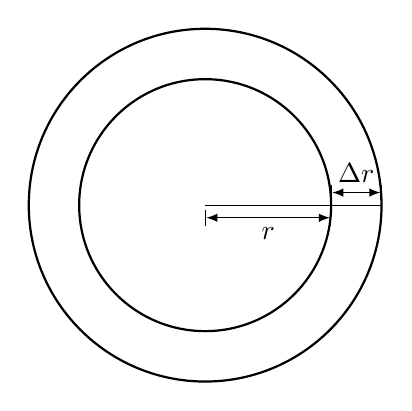
\begin{tikzpicture}[>=latex, scale=.8]
\draw[thick](0,0) circle(2);
\draw[thick](0,0) circle(2.8);
\draw(0,0)--(2.8,0);
\draw[|<->|](0,-.2)--node[below]{$r$}(2,-.2);
\draw[|<->|](2.8,.2)--node[above]{$\Delta r$}(2,.2);
    \end{tikzpicture}
    \caption{}
\end{minipage}
\begin{minipage}[t]{0.48\textwidth}
    \centering
\begin{tikzpicture}[>=latex, scale=.8]
\tkzDefPoints{-1.5/0/A, 1.5/0/B, 2.7/1.2/C, -2.7/1.2/D}
\tkzDrawPolygon(A,B,C,D)
\tkzDefPoints{1.5/1.2/E, -1.5/1.2/F}
\tkzDrawPolygon[pattern=north east lines](A,D,F)
\tkzDrawPolygon[pattern=north west lines](B,C,E)
\node at (0,1.2)[above]{$2\pi(r+\Delta r)$};
\node at (0,0)[below]{$2\pi r$};
\draw[|<->|](3,0)--node[fill=white]{$\Delta r$}(3,1.2);
\end{tikzpicture}
\caption{}
\end{minipage}
\end{figure}

把圆沿半径剖开,把圆周拉直,圆环就“变成”一个梯形,它的两个底边长分别是$2\pi r$, $2\pi(r+\Delta r)$, 高为$\Delta r$(图2.16),其中的矩形面积就是微分$\dd S=2\pi r\cdot \Delta r$, 它表示圆面积$S$在从$r$到$r+\Delta r$的整段变化过程中都以同一瞬时变率$(\pi r^2)'=2\pi r$作匀速变化所产生的面积增量.图2.16中的两个小直角三角形的面积表示$\Delta S$与$\dd S$的误差,即
\[\Delta S-\dd S=\pi  (\Delta r)^2\]
它比$|\Delta r|$更快地变小,即
\[\lim_{\Delta r\to 0}\frac{\Delta S-\dd S}{\Delta r}=\lim_{\Delta r\to 0}\pi(\Delta r)=0\]
\end{solution}

\subsubsection{微分的几何意义}

从几何的观点来说,变率的根本想法就是以直代曲,即以在点$x_0$处的切线$y=f(x_0)+f'(x_0)(x-x_0)$来逼近曲线$y=f(x)$的微段.因此,$f'(x_0)\Delta x$的几何意义可以从图2.17看出.

\begin{figure}[htp]
    \centering
    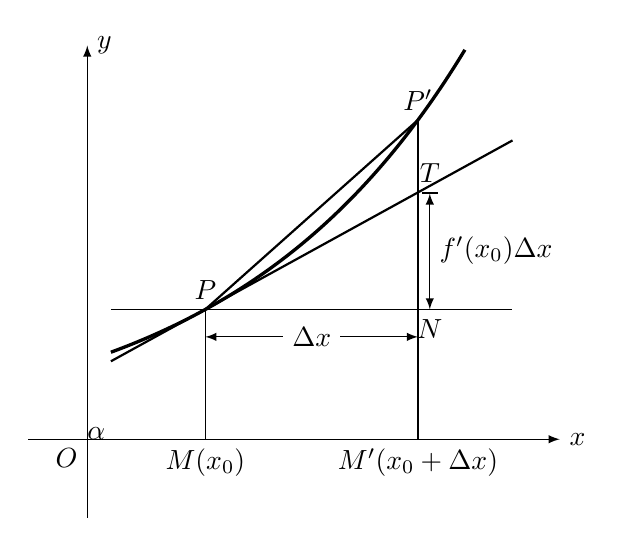
\begin{tikzpicture}[>=latex, xscale=3]
\draw[->](-.25,0)--(2,0)node[right]{$x$};
\draw[->](0,-1)--(0,5)node[right]{$y$};
\node at (0,0)[below left]{$O$};
\draw[domain=.1:1.6, samples=100, very thick]plot(\x, {exp(\x)});
\draw(.5,0)node[below]{$M(x_0)$}--(.5,1.65)node[above]{$P$};
\draw(1.4,0)node[below]{$M'(x_0+\Delta x)$}--(1.4,4.055)node[above]{$P'$};
\draw(.1,1.65)--(1.8,1.65);
\draw[thick](1.4,4.055)--(.5,1.65);
\draw[domain=.1:1.8, samples=10, thick]plot(\x, {1.65*\x+0.825});
\draw[<->](.5,1.3)--node[fill=white]{$\Delta x$}(1.4,1.3);
\draw[<->|](1.45,1.65)node[below]{$N$}--node[right]{$f'(x_0)\Delta x$}(1.45,3.135)node[above]{$T$};
\tkzDefPoints{.5/1.65/P, 1.4/1.65/N, 1.4/3.135/P'}
%\tkzMarkAngle[mark=none, size=.3](N,P,P')
\tkzLabelAngle[pos=.2](N,P,P'){$\alpha$}
    \end{tikzpicture}
    \caption{}
\end{figure}

在直角三角形$TPN$中,$PN=\Delta x$, $\tan\alpha=f'(x_0)$, 故
\[NT=PN\cdot \tan\alpha=\Delta x\cdot f'(x_0)=f'(x_0)\Delta x\]
也就
是切线函数$y=f (x_0) +f' (x_0) (x-x_0)$的相应改变量.至于函数的改变量则是曲线$y=f(x)$本身
的纵坐标在这一段的改变量,在图2.17中用线段$NP'$来代表.所以$f(x)$相应于这一段的微分就是以曲线的切线改变量代替函数的改变量.从图2.17可以看出,当$|\Delta x|$减小时,$TP'$跟着减小,但$TP'$比$|\Delta x|$要变小得更快.

回顾上面的讨论,微分的意义是,当$|\Delta x|$充分小时,曲线$y=f(x)$在点$x_0$的切线
\[y=f (x_0) +f' (x_0) (x-x_0)\]
的改变量$\dd y=f'(x_0)\Delta x=f'(x_0)(x-x_0)$, 就是相应于函数改变量$\Delta y=f(x_0+\Delta x)-f(x_0)$的微分,它可以近似地表达函数改变量,而差是一个比$|\Delta x|=|x-x_0|$变小得更快的微量.因此我们得到
\[\Delta y\approx \dd y\qquad \text{或}\qquad f(x_0+\Delta x)-f(x_0)\approx f'(x_0)\Delta x\]
上式可改写为
\[f (x_0+\Delta x) \approx f (x_0) +f' (x_0) \Delta x\]
可见$f(x)$在$x_0+\Delta x$点的函数值,可以通过它在$x_0$的函数值$f(x_0)$加上一个与$\Delta x$成正比例的量$f'(x_0)\Delta x$来表达,比例系数就是$f$在点$x_0$的微商.上面的公式常用来作近似计算.

\begin{example}
    计算$\sqrt{101}$
\end{example}


\begin{solution}
设$y=\sqrt{x}$,令$x_0=100$, $\Delta x=1$,则
\[\dd y=\frac{\Delta x}{2\sqrt{x_0}}=\frac{1}{2\sqrt{100}}=\frac{1}{20}=0.05\]
因此:
\[\sqrt{101}\approx \sqrt{100}+\dd y=10+0.05=10.05\]
\end{solution}



\begin{example}
一个立方体形状的盒子,它的设计边长等于4(dm), 但允许误差为0.05(dm), 求盒子体积的可能误差.
\end{example}


\begin{solution}
设盒子的边长由$x$改为$x+\dd x$, 那么盒子体积的改变量是
\[\Delta V= (x+\dd x)^3-x^3\]
但是
\[\Delta V\approx \dd V=3x^2\dd x\]
令$x=4$, $\dd x=\pm 0.05$, 那么
\[\dd V=3\x16\x (\pm 0. 05) =\pm 2.4\]
因此,体积的可能误差近似地等于$\pm 2.4({\rm dm})^3$.
\end{solution}

\begin{example}
    证明当$|x|$很小时,$\ln(1+x)\approx x$.
\end{example}

\begin{solution}
    设$f(x)=\ln(1+x)$, 令 $x_0=0$, $\Delta x=x$,则
\[\dd f (x) =f' (x_0) \Delta x=\frac{1}{1+x_0}\Delta x=x\]
因此:
\[f (x_0+\Delta x) =\ln (1+x) \approx \ln 1+x=x\]
即:$\ln(1+x)\approx x$
\end{solution}


\begin{example}
    当$|x|$很小时,导出近似公式:$\tan x\approx x$.
\end{example}


\begin{solution}
    设$f(x)=\tan x$, 令 $x_0=0$, $\Delta x=x$, 则
\[\dd f (x) =\sec^2x_0 \dd x=\sec^2 0\cdot x=1\cdot x=x\]
因此:
\[f (x_0+\Delta x) =\tan x\approx \tan 0+x=x\]
即:$\tan x\approx x$.
\end{solution}

\begin{example}
如图2.18, 加工锥形工件时,已知工件两头直径分别为$d_1,d_2$, 长度为$\ell$, 当斜角$\alpha$很小时,导出近似公式:
\[\alpha=28.6^{\circ}\x\frac{d_1-d_2}{\ell}\]
\end{example}

\begin{figure}[htp]
    \centering
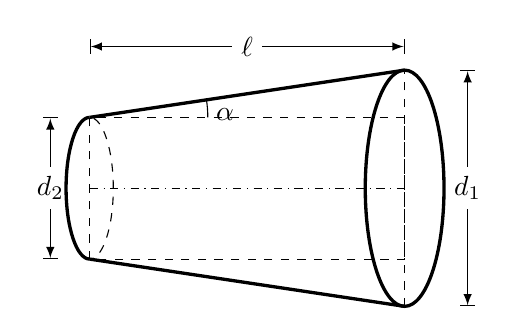
\begin{tikzpicture}[>=latex]
    \draw[|<->|](-0.5,.9)--node[fill=white]{$d_2$}(-.5,-.9);
\draw[|<->|](4.8,1.5)--node[fill=white]{$d_1$}(4.8,-1.5);
\draw[very thick](4,0) ellipse [x radius=.5, y radius=1.5];
\draw[dashed](0,0) ellipse [x radius=.3, y radius=.9];
\draw[dashed](0,-.9) rectangle (4,.9);
\draw[very thick](0,-.9)--(4,-1.5);\draw[very thick](0,.9)--(4,1.5);
\draw[dashdotted](0,0)--(4,0);
\draw[dashed](4,-1.5)--(4,1.5);
\draw[|<->|](0,1.8)--node[fill=white]{$\ell$}(4,1.8);
\draw[very thick] (0,.9) arc [start angle =90, end angle =270, x radius=.3, y radius=.9] ;
\draw (1.5,.9) arc (0:9:1.5)node[below right]{$\alpha$};
\end{tikzpicture}  
    \caption{}
\end{figure}

\begin{solution}
由图:$\tan\alpha=\frac{d_1-d_2}{2\ell}$. 当$\alpha$很小时,根据$\tan\alpha\approx \alpha$,得到:
\[\alpha\approx \frac{d_1-d_2}{2\ell}\]
又:$1\text{弧度}=\left(\frac{180}{\pi}\right)^{\circ}\approx 57.3^{\circ}$,因此:
\[\alpha\approx 57.3^{\circ}\x \frac{d_1-d_2}{2\ell}\approx 28.6^{\circ}\x \frac{d_1-d_2}{\ell}\]
\end{solution}

\subsubsection{微分的运算}

如果函数$f(x)$可微,即导数$f'(x)$存在,求函数的微分只要求出导数再乘以自变量的改变量$\Delta x$就行了,求已知函数的微分或求导数的方法都叫做微分法.

我们已经知道当$x$是自变量时,$\dd x=\Delta x$, 原来的微分表达式$\dd y=f'(x)\Delta x$就可以改写为$\dd y=f'(x)\dd x$, 例如$\dd(\sin x)=\cos x \dd x$. 所以我们可以根据函数的和、积、商的求导数法则得到函数的和、积、商的求微分法则,即
\begin{enumerate}
    \item $\dd(cu)=c\dd u$
    \item $\dd(u\pm v)=\dd u\pm \dd v$
    \item $\dd(uv)=v\dd u+u\dd v$
    \item $\dd\left(\frac{u}{v}\right)=\frac{v\dd u-u\dd v}{v^2}$
\end{enumerate}
这里只证明最后一个法则,其余请读者自证.

\begin{proof}
\begin{align*}
\dd\left(\frac{u}{v}\right)=\left(\frac{u}{v}\right)'\dd x&=\frac{u'v-uv'}{v^2}\dd x\\
&=\frac{v(u'\dd x)-u(v'\dd x)}{v^2}\\
&=\frac{v\dd u-u\dd v}{v^2}
\end{align*}
\end{proof}


现在我们来研究求复合函数的微分法则.

如果$y=f(x)$, $x=\varphi (t)$, 那么$y$是$t$的复合函数$y=f(\varphi (t))$, 这时$x$和$y$的微分根据定义都要以$t$为自变量来确定.在这情况下,须注意$\dd x\ne \Delta x$, 比如若$x=t^2$, 则$\dd x=2t\dd t$, 而$\Delta x=(t+\Delta t)^2-t^2=2t\Delta t+(\Delta t)^2$, 显然$\dd x\ne \Delta x$, 对于复合函数$y=f(\varphi (t))$的微分,我们有下面重要定理.

\begin{blk}
    {定理} 设$y=f(x)$, $x=\varphi (t)$都是可微函数,$x$是中间变量,那么关系式
$\dd y=f (x) \dd x$
仍成立.
\end{blk}

\begin{proof}
   \[ \dd y=[f(\varphi (t))]'\dd t\]
根据复合函数求导数法则有
\[[f (\varphi  (t) ) ] '=f' (\varphi  (t) ) \cdot \varphi ' (t)\]
因此
\[\dd y=f' (\varphi  (t) ) \cdot \varphi' (t) \dd t\]

因为$x=\varphi  (t)$, $\dd x=\varphi ' (t) \dd t$,最后得到
\[\dd y=f' (x) \dd x\]
\end{proof}

这个定理是说不论$x$是自变量或是中间变量,函数$f(x)$
的微分形式不变,只须注意,若$x$是中间变量,$\dd x$不是任意增量$\Delta x$, 而是$x$的微分,$\dd y$不能写成$f'(x)\Delta x$即$\dd y\ne f'(x)\Delta x$, 这个性质叫做\textbf{微分不变性}.有了微分不变性,我们在作微分运算时,就无需指明对哪一个变量的微分,而在求函数的变率时,总要指明对中间变量求导数还是对自变量求导数.另外,求复合函数的导数法则用微分符号写出,就是
\[\frac{\dd y}{\dd t}=\frac{\dd y}{\dd x}\cdot \frac{\dd x}{\dd t}\]
它就成为简单的代数恒等式了.

\begin{example}
    求由方程$y^3=x^2+xy+y^2$确定的隐函数的导数$\frac{\dd y}{\dd x}$.
\end{example}

\begin{solution}
    对等式两边求微分得到
\[3y^2\dd y=2x\dd x+ (x\dd y+y\dd x) +2y\dd y\]
移项
\[(3y^2-x-2y)\dd y=(2x+y)\dd x\]
最后得到
\[\frac{\dd y}{\dd x}=\frac{2x+y}{3y^2-x-2y}\]
\end{solution}

\begin{example}
    求$\dd\sin [\tan(x^2-x+1)]$.
\end{example}


\begin{solution}
\begin{align*}
    \dd\sin \left[\tan(x^2-x+1)\right]&=\cos\left[\tan(x^2-x+1)\right]\dd \tan(x^2-x+1)\\
    &=\cos\left[\tan(x^2-x+1)\right]\cdot \sec^2 (x^2-x+1)\cdot \dd (x^2-x+1)\\
    &=\cos\left[\tan(x^2-x+1)\right]\sec^2(x^2-x+1)\cdot (2x-1)\dd x 
\end{align*}
\end{solution}
(例2.52的计算中,将微分符号“$\dd$”逐步顺着复合函数
的层次从$\sin$到$\tan$到$x^2-x+1$, 由外到里,尤如剥笋.)


\begin{ex}
\begin{enumerate}
    \item 边长4cm的正方形铁皮,在加热中边长增加了0.001cm, 
求此时刻面积的可能误差$\Delta S$, 和可能误差的近似值$\dd s$, 又正方形的面积近似值是多少?
\item 半径为10cm的球,在冷却中$R$缩短了0.001cm, 求此时
刻体积的微分$\dd V$和体积的近似值.
\item 当$|x|$很小时,导出下列近似公式:
\begin{multicols}{2}
\begin{enumerate}
    \item  $\sqrt{1+x} \approx 1+\frac{x}{2}$
\item $e^{x} \approx 1+x$
\item  $(1+x)^{n} \approx 1+n x$
\item  $\sqrt[n]{1+x} \approx 1+\frac{1}{n} x$
\item  $\sin x \approx x$
\item  $\arcsin x \approx x$
\item  $\ln (1+\sin x) \approx x$
\end{enumerate}
\end{multicols}

\item  计算下列各式的值:
\begin{multicols}{2}
\begin{enumerate}
\item  $\sqrt[3]{1.02}$
\item  $\sqrt[3]{0.998}$
\item   $e^{-0.1}$
\item   $\tan 0.01$ 
\item   $\sin 0.1^{\circ}$
\item   $\ln 1.0021$   
\end{enumerate}
\end{multicols}

\item 求下列函数的徽分:
\begin{multicols}{2}
\begin{enumerate}
    \item $y=\frac{x+5}{x^{2}-2}$
    \item  $y=\left(\sqrt{1+x^{2}}\right)^{n}$
    \item  $y=\ln (\sin \sqrt{x})$
    \item  $y=\sin ^{3}(\sqrt{x})$
    \item  $y=\arcsin \sqrt{2 x}$
    \item  $y=\arctan (\cos x)$ 
    \item $y=\sin (\ln x)$
    \item $y=x^{n} \ln (n x)$
    \item $y=e^{x} \ln x$
    \item $y=\left(e^{x}+e^{-x}\right)^{2}$
\end{enumerate}
\end{multicols}

\item 一直圆锥内接于半径等于$R$的球中,球心在直圆锥的内部
且到圆锥底面的距离等于$p$, 若$p$增加一个微量$x$而球半径$R$不变,求证圆锥体积的增量约等于$\frac{\pi}{3}(R+p)(R-3p) x$.
\item 直圆锥的底面半径为$r$ cm, 高为$h$ cm, 若半径$r$和高$h$分别
有一个增量$\rho$ cm和$\lambda$ cm, 求证圆锥体积的增量近似地等于$\left(\frac{2\rho}{r}+\frac{\lambda}{h}\right)$.
\end{enumerate}
\end{ex}

\subsection*{习题2.2}
\begin{enumerate}
    \item 求下列函数的导函数:
	\begin{enumerate}
    	\begin{multicols}{2}
			\item $f(x)=2 x^{3}-3 x^{3}+4 x-5 $
			\item $f(x)=x^{5}-6 x^{2}+13$
			\item $f(x)=\frac{x^{3}-4 x}{x^{2}+1} $
			\item $f(x)=\cos m x \sin n x$       
    	\end{multicols}

		\item $f(x)=\left[\sin x+\cos x+\left(x^{2}+x+1\right)\right]^{2}$
		\item $f(x)=\tan\left[\sin x+\cos x+\left(x^{2}+x+1\right)\right]$
		\begin{multicols}{2}
			\item $f'(x)=\cot \left(x^{2}+1\right)$
			\item $f(x)=\sqrt{a^{2}+b^{2} x^{2}}$
			\item $f(x)=\sqrt[3]{x^{4}+x^{2}+1}$
			\item $f(x)=\cos \left(\sqrt[3]{3 x^{4}+5 x^{2}+6}\right)$
			\item $f(x)=(\sqrt{x}+1)\left(\frac{1}{\sqrt{x}}-1\right)$
			\item $f(x)=x \sin x+\cos x$
			\item $f(x)=2^{\sin ^{2}\tfrac{1}{x}} $
			\item $f(x)=x^{\sin x}$       
		\end{multicols}
		\begin{multicols}{2}
		\item $f(x)=e^{-x^{2}} \cos \left(e^{-x^{2}}\right) $
		\item  $f(x)=\arctan\sqrt{x^{2}-2 x}$
		\item  $f(x)=x e^{1-\cos x}$
		\item  $f(x)=x \arccos x-\sqrt{1-x^{2}}$
		\item  $f(x)=(\sin x)^{\cos x}$
		\item  $f(x)=\sqrt[5]{\frac{x-5}{\sqrt[5]{x^{2}+2}}}$
		\end{multicols}
		\item  $f(x)=x-\ln \left(2 e^{x}+1+\sqrt{e^{2 x}+4 e^{x}+1}\right)$
		\begin{multicols}{2}
		\item $f(x)=\sqrt{x \sqrt{x \sqrt{x}}}$
		\item  $f(x)=\log _{a} e ^{\sin ^{2} x+1}$
		\end{multicols}
		\item  $f(x)=\ln \tan  \frac{x}{2}-\cot x \cdot \ln (1+\sin x)-x$
	\end{enumerate}

\item 验证函数$f(x)=e^x \sin x$满足方程
\[f'' (x) -2f' (x) +2f (x) =0.\]

\item 验证函数$f(x)=\frac{x-3}{x+4}$满足方程
\[2 [f' (x) ]^2= [f (x) -1] f'' (x).\]

\item $P$点在直线上运动,在时刻$t$, 点$P$与直线上的定点$O$的距离由方程
$s^2=a^2+V^2t^2$
给出,其中$a$和$V$是常量,试用$s$表示$P$点在时刻$t$的速度和加速度.

\item 在$xy$平面上,求通过点$P(-3, 6)$且与曲线$y=x^3-5x^2+x+5$
相切,并且切点的横坐标满足$x\ge 0$的切线方程.

\item 求证方程$16x^4-24x^2+16x-3=0$在$(0, 1)$内有
一个三重根,又在$(-2,-1)$内有一个单根.

\item 设三次函数$y=x^3-3ax^2+bx+c$ (其中$a,b,c$是
常数).
\begin{enumerate}
    \item 该曲线与直线$y=2x-1$切于点$(2, 3)$, 试用$a$的式子表示$b,c$;
    \item 另外,该曲线还与$y=2x+3$相切,试确定$a,b,c$的值.
\end{enumerate}
\item 在中午十二点整,甲船以6公里/小时的速率向东行,乙船在甲船之北16公里,以8公里/小时的速率向南行,在下午一点整两船相近之速率为多少?在下午两点整两船相离之速率是多少?
\item 已知圆心为$O$, 半径为1的圆与直线$\ell$相切于点$A$, 一动点$P$自切点$A$沿直线$\ell$向右移动时,取弧$\wideparen{AC}$的长为$\frac{2}{3}AP$,
直线$PC$与直线$AO$交于点$M$(图2.19), 又知当$AP=\frac{3\pi}{4}$时,点$P$的速率为$v$, 求这时$M$点的速率.

\begin{figure}[htp]
    \centering
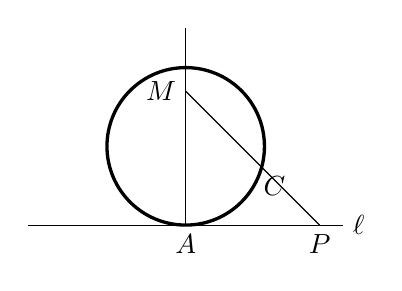
\begin{tikzpicture}
\draw(-2,0)--(2,0)node[right]{$\ell$};
\draw[very thick](0,1) circle (1);
\draw(0,0)node[below]{$A$}--(0,2.5);
\draw(0,1.7)node[left]{$M$}--(1.7,0)node[below]{$P$};
\node at (30:1)[right]{$C$};
\tkzDefPoints{0/1/O}
\tkzLabelPoints[left](O)
\tkzDrawPoints(O)

\end{tikzpicture}    
    \caption{}
\end{figure}

\item 溶液自深18cm, 顶直
径12cm的正圆锥形漏斗中漏入一直径为10cm的圆柱形筒中,开始时漏斗中盛满了水,已知当溶液在漏斗中深为12cm时,其水平面下落速率为1cm/s, 问此时圆柱形筒中水平面上升之速率为多少?
\item 求曲线$y=\arctan\ln x$与$x$轴的交角.
\item 设质点$P$在时刻$t$的位移方程是
\[x=\frac{58}{240}+A\cos\left(\sqrt{24}gt+\alpha\right)\]
其中$A,\alpha$是待定常数,$g\approx 9.8{\rm m/s}$,且知当$t=0$时,$x=0$, $\frac{\dd x}{\dd t}=0$,求$A$和$\alpha$.


\begin{figure}[htp]
    \centering
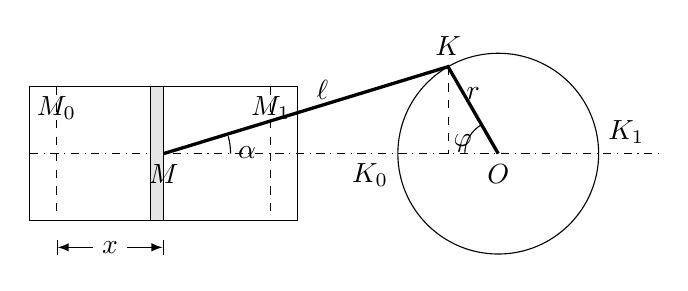
\begin{tikzpicture}[>=latex, scale=1.7]
    \draw[dashdotted] (-3.5,0)--(1.2,0);
    \draw (-3.5,.5) rectangle (-1.5,-.5);
    \draw (0,0) circle (.75);
    \node at (-.75,0)[below left]{$K_0$};
    \node at (.75,0)[above right]{$K_1$};
\draw [fill=gray!20](-2.5,.5) rectangle (-2.6,-.5);
\draw[very thick] (0,0)node[below]{$O$}--node[above]{$r$}(90+30:.75)node[above]{$K$}--node[above right]{$\ell$}(-2.5,0)node[below]{$M$};
\draw [dashed](-3.3,.5)node[below]{$M_0$}--(-3.3,-.5);
\draw [dashed](-1.7,.5)node[below]{$M_1$}--(-1.7,-.5);
\draw (-.25,0) arc (180:180-60:.25)node[below left]{$\varphi$};
\draw[dashed] (90+30:.75)--(-.75/2,0);
\draw[|<->|] (-3.3,-.7)--node[fill=white]{$x$}(-2.5,-.7);

\draw (-2,0) arc (0:15:.5)node[below right]{$\alpha$};


\end{tikzpicture}
    \caption{}
\end{figure}



\item 图2.20表示曲柄机构装置的图样,连接杆$MK$
的长$\ell=125$cm, 曲柄$OK$的长$r=25$cm, 连杆与汽缸的轴$OM$成$\alpha$角,曲柄与同一轴成$\varphi$角.
\begin{enumerate}
    \item 求用$\varphi$的式子表示活塞$M$的位移$x$的公式;
    \item 如果$\frac{\dd \varphi}{\dd t}=\omega$ ($\omega$
    是常量),求活塞$M$的速率.
\end{enumerate}
\item 在抛物线$y=ax^2+bx+c\; (a\ne 0)$上两点作切线,
它们在何处相交?
\item 求抛物线$y^2=4ax$在点$(a\lambda^2, 2a\lambda)$的切线方程,并求它的两条互相垂直的切线的交点的轨迹方程.
\item 
\begin{enumerate}
    \item 求曲线$4y^3=27x^2$ 在点$(2t^3, 3t^2)$的切
线方程;
\item 求互相垂直的两条切线的交点的轨迹方程.
\end{enumerate}

\item 计算$\sqrt{\frac{2.037^2-1}{2.037^2+1}}$的近似值.
\item 计算$\cos151^{\circ}$的近似值.
\item 设$f(x)=e^{0.1x(1-x)}$, 试计算$f(1.05)$的近
似值.
\item 若球体积的相对误差$\frac{\Delta V}{V}=0.01$, 试计算球半径的
相对误差$\frac{\Delta R}{R}$约等于多少?
\end{enumerate}


\section{微商运算的初步应用{}---{}函数的增减与极值}

\subsection{局部极值和中值定理}
我们在第一章中曾说明在闭区间$[a,b]$上连续的函数必有最大值和最小值.函数$f$在闭区间$M=[a,b]$上的最大值的大小涉及到两个因素,既依赖于$f$,也依赖于$M$.

如图2.21,若$N=[c,d]\subset M=[a,b]$,则
\[
\max_N f \le \max_M f.
\]
相应地,
\[
\min_N f \ge \min_M f.
\]
在这两种情形里都可能出现严格不等式(即不带等号的不等式).

\begin{figure}[htp]
    \centering
    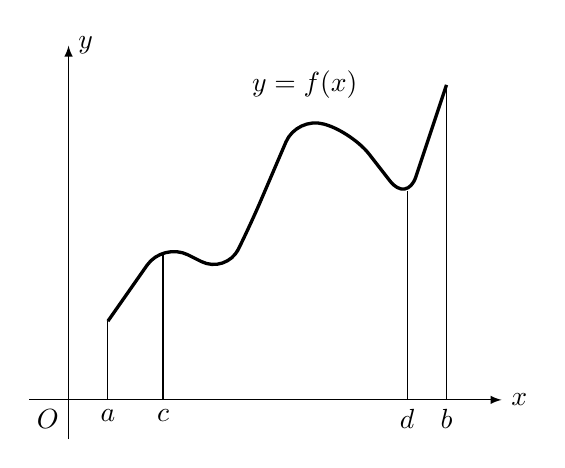
\begin{tikzpicture}[>=latex]
        \draw[->](-.5,0)--(5.5,0)node[right]{$x$};
        \draw[->](0,-.5)--(0,4.5)node[right]{$y$};
        \node at (0,0)[below left]{$O$};
        \draw[rounded corners=10pt, very thick](.5,1)--(1.2,2)--(2,1.6)--(2.3,2.2)--(2.9,3.6)--(3.6,3.4)--(4.3,2.5)--(4.8,4);
        \node at (3,4){$y=f(x)$};
        \draw(.5,1)--(.5,0)node[below]{$a$};
        \draw(1.2,1.85)--(1.2,0)node[below]{$c$};
        \draw(4.3,2.65)--(4.3,0)node[below]{$d$};
        \draw(4.8,4)--(4.8,0)node[below]{$b$};
        \end{tikzpicture}
    \caption{}
\end{figure}

现在我们将阐明一种只决定于$f$的性质的局部极大与极小的概念.

\begin{blk}
    {定义} 设函数$f$在点$x$的某个$\delta>0$的邻域,即$(x-\delta,x+\delta)$内有定义,如果对于充分小的$|\Delta x|<\delta$, 能使$x+\Delta x\in (x-\delta,x+\delta)$, 而且对于一切$x'=x+\Delta x\in (x-\delta,x+\delta)$, 都有
\[f(x+\Delta x)\le f(x)\quad \text{或}\quad f(x+\Delta x)\ge f(x)\]
那么函数$f$在点$x$达到局部极大值(或局部极小值).
\end{blk}

\begin{blk}
    {费马定理} 如果函数$f$在区间$(a,b)$上有定义,并且在这个区间内的一点$c$取局部极大值(或极小值),又若$f$在$c$点可微,那么
    \[f' (c) =0\]
\end{blk}

\begin{proof}
    为确定起见,设$f(x)$在点$c\in (a,b)$取最大值、于是对于一切点$x\in (a,b)$, 就有
\[
f (x) \le f (c). 
\]
由导数定义:
\[\lim_{x\to c}\frac{f (x) -f (c)}{x-c} =f' (c) \]
并且极限$f'(c)$的存在与$x$是从右边还是从左边趋向$c$无关.

\begin{enumerate}
    \item 如果$x>c$,我们有$\frac{f (x) -f (c)}{x-c}\le 0$,从而
\[\lim_{x\to c^+}\frac{f (x) -f (c)}{x-c}\le 0\]
\item 如果$x<c$,我们有$\frac{f (x) -f (c)}{x-c}\ge 0$,从而
\[\lim_{x\to c^-}\frac{f (x) -f (c)}{x-c}\ge 0\]
\end{enumerate}
根据假设$f$在$c$点可微,因此这两个极限必相等,且应等于$f'(c)$, 这表示$f'(c)\ge 0$和$f'(c)\le 0$, 由此得:$f' (c) =0$.

$f$在$c$点有局部极小值的情形留给读者自证.
\end{proof}

\begin{blk}
  {罗尔定理} 如果函数$f$在闭区间$[a,b]$上连续,在开区间$(a,b)$内可微,且在两端点的函数值相等,即$f(a)=f(b)$, 那么至少存在一个点$c$, $c\in (a,b)$, 使$f'(c)=0$.  
\end{blk}

\begin{proof}
如果$f$在$[a,b]$上恒为常数,无疑对于任何
$c\in (a,b)$有$f'(c)=0$. 因此,可设$f$在$[a,b]$中不为常数,此时$f$在$[a,b]$上的最大值$M$和最小值$m$至少有一个不等于$f(a)=f(b)$, 为确定起见,不妨设$M\ne f(a)=f(b)$.故$f$在$[a,b]$上的最大值$M$不会在$a$点或$b$点达到,这时根据闭区间上连续函数的性质,在$(a,b)$内至少有一点$c$, 使$f(c)=M$, 于是,由费马定理,即得$f'(c)=0$. 

本定理的几何意义如图2.22, 曲线$y=f(x)$在$a,b$处有相同高度,如果在点$c$处、曲线达到最高度,并有切线存在,那么,曲线在该处的切线与$x$轴平行.同样,在曲线的最低点处的切线也与$x$轴平行.
\end{proof}

\begin{figure}[htp]
    \centering
    \begin{minipage}[t]{0.48\textwidth}
    \centering
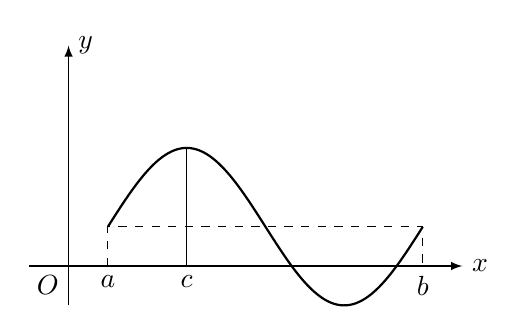
\begin{tikzpicture}[>=latex, scale=1]
    \draw[->](-.5,0)--(5,0)node[right]{$x$};
    \draw[->](0,-.5)--(0,2.8)node[right]{$y$};
    \node at (0,0)[below left]{$O$};
    \draw[domain=.5:4.5, samples=100, thick]plot(\x, {sin((\x-.5)*pi/2 r)+.5});
    \draw[dashed](.5,0)node[below]{$a$}--(.5,.5)--(4.5,.5)--(4.5,0)node[below]{$b$};
    \draw(1.5,0)node[below]{$c$}--(1.5,1.5);
\end{tikzpicture}
    \caption{}
    \end{minipage}
    \begin{minipage}[t]{0.48\textwidth}
    \centering
    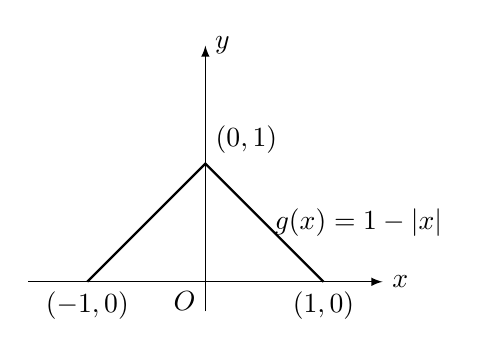
\begin{tikzpicture}[>=latex, scale=1.5]
        \draw[->](-1.5,0)--(1.5,0)node[right]{$x$};
        \draw[->](0,-.25)--(0,2)node[right]{$y$};
        \draw[thick](-1,0)node[below]{$(-1,0)$}--(0,1)node[above right]{$(0,1)$}--node[right]{$g(x)=1-|x|$}(1,0)node[below]{$(1,0)$};
        \node at (0,0)[below left]{$O$};
    \end{tikzpicture}
    \caption{}
    \end{minipage}
    \end{figure}


\begin{rmk}
    注意 如果罗尔定理中的条件不被满足,结论就不成立.例如$g(x)=1-|x|$在$[-1, 1]$上连续,且$g(-1)=g(1)=0$, 但在$x=0$处,$g'(x)$不存在,对于这个$g$, 在$(-1,1)$中就设有$c$能使$g'(c)=0$. 它的图象如图2.23所示,
\end{rmk}

\begin{blk}
    {拉格朗日中值定理} 如果函数$f$在闭区间$[a,b]$上连续,在开区间$(a,b)$内可导,那么在$(a,b)$内至少有一点$c$, 使得
\[f'(c)=\frac{f(b)-f(a)}{b-a}\]
\end{blk}

罗尔定理是拉格朗日定理的特殊情形,我们借助于罗尔定理来证明这个重要的定理.

\begin{proof}
 我们作一个辅助函数$\Phi$使它具有函数f的性质:即它在$[a,b]$上连续且在$(a,b)$内可微,同时满足$\Phi (a)=\Phi (b)$. 为此,设$\Phi  (x) =f (x) +k (x-a)$, 并由条件$\Phi (a)=\Phi (b)$来决定参数$k$. 

因为当$x=a$时,有$\Phi (x)=f(a)$; 当$x=b$时,有$\Phi (b)=f(b)+k(b-a)$, 所以
\[k=-\frac{f (b) -f (a)}{b-a}\]
这样得到的函数
\[\Phi  (x) =f (x) -\frac{f (b) -f (a) }{b-a}(x-a)\]
就满足罗尔定理中的所有的条件,由罗尔定理,至少存在一点$c\in (a,b)$使得$\Phi '(c)=0$,
但
\[\Phi ' (x) =f' (x) -\frac{f (b) -f (a)}{b-a}\]
所以
\[\Phi ' (c) =f' (c) -\frac{f (b) -f (a)}{b-a} =0\]
即
\[f' (c) =\frac{f (b) -f (a)}{b-a}\]
\end{proof}

为了便于应用,拉格朗日定理的结论,通常写成如下形式:
\begin{equation}
   f (b) -f (a) =f' (c) (b-a),\qquad a<c<b 
\end{equation}
在上式中,令$b=a+h$,$c=a+\theta h$,$0<\theta<1$,得到中值定理的另一形式:
\begin{equation}
    f (a+h) -f (a) =hf' (a+\theta h) ,\qquad 0<\theta<1
\end{equation}

中值定理的几何意义如图2.24所示.在闭区间$[a,b]$上有一条连续的曲线,且过曲线$y=f(x)$上每一点(端点除外),都可以作出一条切线,那么在曲线上至少有一点$M(c, f( c)),\; c\in (a,b)$, 使得过点$M$的切线与弦$AB$平行.

\begin{figure}[htp]
    \centering
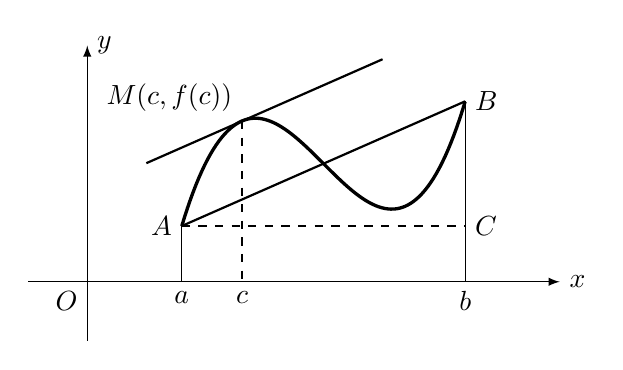
\begin{tikzpicture}[>=latex, scale=1.5]
\draw[->](-.5,1)--(4,1)node[right]{$x$};
\node at (0,1)[below left]{$O$};
\draw[->](0,.5)--(0,3)node[right]{$y$};
\draw[domain=.8:3.2, samples=100, very thick]plot(\x, {(\x-1)*(\x-2)*(\x-3)+2});
\draw(.8,1)node[below]{$a$}--(.8,1.472)node[left]{$A$};
\draw(3.2,1)node[below]{$b$}--(3.2,2.528)node[right]{$B$};
\draw[thick](.8,1.472)--(3.2,2.528);
\draw[dashed](.8,1.472)--(3.2,1.472)node[right]{$C$};
\draw[dashed](1.31,2.3603)node[above left]{$M(c,f(c))$}--(1.31,1)node[below]{$c$};

\draw[domain=.5:2.5, samples=10, thick]plot(\x, {0.44*\x+1.784});

\end{tikzpicture}
    \caption{}
\end{figure}



\begin{example}
求$f(x)=1+\frac{4}{x}$在$(1, 4)$内满足中值定理$f(b)-f(a)=f'(c)\cdot (b-a)$的点$c$的值.
\end{example}


\begin{solution}
    显然$f$在$[1, 4]$上连续,又$f'(x)=-\frac{4}{x^2}$, 故$f$在$(1, 4)$内可微,根据中值定理,存在点$c\in (1, 4)$, 使得
\[    f (4) -f (1) = (4-1) f' (c)\]
成立.

$\because\quad f (4) =2,\quad f (1) =5$,

$\therefore\quad 2-5=3 \left(-\frac{4}{c^2}\right),$
即:$c^2=4$,得$c=\pm 2$.

又$\because\quad 2\in (1, 4),\quad -2\notin (1, 4)$,

$\therefore\quad c=2$. 于是
\[    f (4) -f (1) = (4-1) f' (2) \]
\end{solution}

\begin{example}
    设$f(x)=a_0+a_1x+a_2x^2+\cdots+a_nx^n$, 求证在$f'(x)=0$的相邻二根之间,至多有$f(x)=0$的一个根.   
\end{example}

\begin{proof}
因为多项式函数处处连续和可微,所以若在$f'(x)=0$的两相邻实根$x_1,x_2$之间有$f(x)=0$的二实根$\alpha,\beta\; (\alpha<\beta)$, 那么根据罗尔定理,至少存在$f'(x)=0$的一个根$c$, 使得$\alpha<c<\beta$.但是$(\alpha,\beta)\subset (x_1,x_2)$,于是$x_1<c<x_2$,由此得出矛盾,所以在$f'(x)=0$的相邻两根之间,至多有$f(x)=0$的一个根.
\end{proof}

\begin{example}
    求证不等式$\frac{h}{1+h}<\ln(1+h)<h$,
    对于$h\in (-1, 0)\cup (0,+\infty)$成立.
\end{example}


\begin{proof}
    设$f(x)=\ln x$, 于是$(\ln x)'=\frac{1}{x}$. 由于$\ln x$在区间$[a,b],\; (0<a<b)$上连续且在$(a,b)$内可微,根据中值定理$(a,b)$内存在$c$,使得:
\begin{equation}
    \ln b-\ln a=\frac{1}{c}(b-a),\quad a<c<b
\end{equation}

若$h>0$, 令$a=1$, $b=1+h$, 于是$c=1+\theta h$, 这样(2.26)可写成
\[\ln (1+h) =\frac{h}{1+\theta h},\quad 0<\theta<1\]
若把上式中的$\theta$看作变数,由0变到1, 那么$\ln(1+h)=\frac{h}{1+\theta h}=\frac{1}{\frac{1}{h}+\theta}$
便由$h$递减到$\frac{h}{1+h}$,所以
\[h>\ln(1+h)>\frac{h}{1+h},\quad h>0\]

若$-1<h<0$,令$a=1+h$,$b=1$,于是$c=1+\theta h$,这样
(2.26)可以写成
\[\ln1-\ln (1+h) =\frac{-h}{1+\theta h}\]
仍得
\[\ln (1+h) =\frac{h}{1+\theta h}\]
同样可证
\[h> \ln (1+h) >\frac{h}{1+h}\]
因此,当$h>-1$且$h\ne 0$时,不等式
\[\frac{h}{1+h}<\ln(1+h)<h\]
成立.
\end{proof}



\begin{ex}
\begin{enumerate}
    \item 曲线$y=x^2$上的某点的切线平行于连接横坐标为$a,b$两点的弦,求出此点.
    \item 曲线$y=\frac{1}{x}$上的某点的切线平行于连接横坐标为$a,b\;(0<a<b)$两点的弦,求出此点.
    \item 若$\varphi(x)=(x-a)^m(x-b)^n$,验证罗尔定理成立.
    \item 用罗尔定理证明,无论$m$为何值,多项式函数$f_m(x)=x^3-3x+m$在$[0, 1]$之间至多有一个根.
    \item 证明下列不等式:
\begin{enumerate}
    \item $|\sin x-\sin y|\le |x-y|$
    \item $\frac{a-b}{a}<\ln \frac{b}{a}<\frac{a-b}{b},\quad 0<b<a$
    \item $\frac{h}{1+h^2}<\arctan h<h,\quad h>0$
    \item 若$0<m<1$,且$x>1$,则:$\frac{m(x-1)}{x^{1-m}}<x^m-1<m(x-1)$
    
    (提示:利用中值定理形式1,取$b=x,\; a=1$)
    \item 若$h>-1$,$h\ne 0$,$n>1$,则:$(1+h)^{\tfrac{1}{n}}<1+\frac{h}{n}$
    \item 若$h>-1$,$h\ne 0$,则:$1-\frac{h}{2}<\frac{1}{\sqrt{1+h}}<1-\frac{h}{2\sqrt{(1+h)^3}}$
\end{enumerate}
\item 说明方程$3x^5-25x^3+60x-20=0$有三个实数根,给出根所在的区间,使每个区间只含一个根.
\end{enumerate}
\end{ex}

\subsection{函数的增减与极值——中值定理的应用}

\subsubsection{函数的增减性}

我们已经学过增函数与减函数的概念,现在要阐明导数的正负与函数的增减的关系.

读者已经知道常量的导数等于零,现在反过来问:如果
函数$f$在给定区间上的导数永远是零,那么这个函数在这个区间上就是一个常量?由拉格朗日定理可得到肯定的回答.

\begin{blk}
  {定理1} 如果函数$f$在开区间$(a,b)$上的每一点的导数等于零,即$f'(x)=0$, 那么函数$f$在$(a,b)$上是一个常数.  
\end{blk}

\begin{proof}
  我们从区间$(a,b)$中固定某一点$x_0$, 再取其它的任何一点$x\in (a,b)$. 对于区间$[x_0,x]$或$[x,x_0]$, 函数$f$满足拉格朗日定理条件,因此,我们可以写出
  \[f (x) -f (x_0) =f' (c) (x-x_0),\qquad c\in (x_0,x)\text{ 或 }(x,x_0)\]
  也就是$c\in (a,b)$, 依已知条件$f'(c)=0$, 因而对任何一点$x\in (a,b)$, $f(x)=f(x_0)=$常数.  
\end{proof}



\begin{example}
    求证:如果$x>1$,那么$2\arctan x+\arcsin\frac{2x}{1+x^2}=\pi$成立.
\end{example}

\begin{proof}
设$f(x)=2\arctan x+\arcsin\frac{2x}{1+x^2}$,因为当$x>1$时,$\left|\frac{2x}{1+x^2}\right|<1$,故对于所指定的$x$值的范围,$f(x)$有定义,又因为:
\begin{align*}
    f'(x)&=2(\arctan x)'+\left(\arcsin\frac{2x}{1+x^2}\right)'\\
    &=\frac{2}{1+x^2}+\frac{1}{\sqrt{1-\left(\frac{2x}{1+x^2}\right)^2}}\cdot \left(\frac{2x}{1+x^2}\right)'\\
    &=\frac{2}{1+x^2}+\frac{1}{\sqrt{1-\left(\frac{2x}{1+x^2}\right)^2}}\cdot \frac{(1+x^2)\cdot 2-2x(2x)}{(1+x^2)^2}\\
    &=\frac{2}{1+x^2}+\frac{2(1-x^2)}{(x^2-1)(1+x^2)}\\
    &=2\left(\frac{1}{1+x^2}-\frac{1}{1+x^2}\right)=0
\end{align*}
所以:
\[2\arctan x+\arcsin\frac{2x}{1+x^2}=c\; \text{(常数)}\]
另一方面,因为
\[f\left(\sqrt{3}\right)=2\arctan\sqrt{3}+\arcsin\frac{\sqrt{3}}{2}=\frac{2\pi}{3}+\frac{\pi}{3}=\pi\]
因此:
\[2\arctan x+\arcsin\frac{2x}{1+x^2}=\pi,\quad (x>1)\]
\end{proof}


\begin{blk}
    {定理2} 若$f(x)$在$[a,b]$连续,在$(a,b)$内$f'(x)>0$ (或$f'(x)<0$),那么$f(x)$在$[a,b]$上严格递增(或严格递减).
\end{blk}


\begin{proof}
    设$a\le x_1<x_2\le b$,由于在闭区间$[x_1,x_2]$上满足拉格朗日定理的条件,因此,在开区间$(x_1,x_2)$上可以找到点$c$,使得
\[f(x_2)-f(x_1)=(x_2-x_1)f'(c)\quad (x_1<c<x_2)\]
根据条件,如果在$(a,b)$内,$f'(x)>0$ (或$f'(x)<0$), 那么$f'(c)>0$ (或$f'(c)<0$), 从而
\[f(x_2)-f(x_1)>0\quad (\text{或}<0)\]
因为对于任意$x_1$和$x_2$ (其中$a\le x_1<x_2\le b$),上面不等式成立,所以$f(x)$在$[a,b]$上严格递增(或严格递减).
\end{proof}

定理2的几何意义是明显的,$f'(x)$是函数图象上点$x$处的切线的斜率$\tan\theta$, 这里$0\le\theta \le \pi$. 这斜率的符号指出切线是向上或向下倾斜的,而曲线本身也就随着它向上升或向下降.

如果$f'(x)$在个别的$x$值等于零,其他条件不变,则定理
2仍然成立,这一点很容易证实,就是把区间$[a,b]$用使$f'(x)=0$的点来分成若干个小区间,再在每个小区间上分别应用定理2. 图2.25和2.26表示定理2的几何意义.

\begin{figure}[htp]
    \centering
    \begin{minipage}[t]{0.48\textwidth}
    \centering
    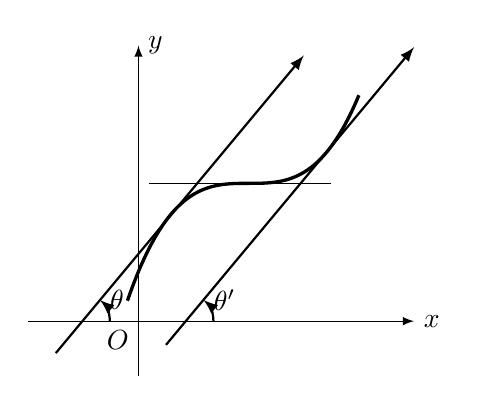
\begin{tikzpicture}[>=latex, scale=.7]
  \draw[->](-2,0)--(5,0)node[right]{$x$};
\draw[->](0,-1)--(0,5)node[right]{$y$};
\node at (0,0)[below left]{$O$};
\draw[domain=-.2:4, samples=100, very thick]plot(\x, {.2*(\x-2)^3+2.5});
\draw[->, domain=-1.5:3, thick, samples=10]plot(\x, {1.2*\x+1.22});
\draw[->, domain=.5:5, thick, samples=10]plot(\x, {1.2*\x-1.03});
\draw(.2,2.5)--(3.5,2.5);
\draw[->, thick](.86+.5,0) arc (0:50.2:.5)node[right]{$\theta'$};
\draw[->, thick](-1.02+.5,0) arc (0:50.2:.5)node[right]{$\theta$};
    \end{tikzpicture}
    \caption{}
    \end{minipage}
    \begin{minipage}[t]{0.48\textwidth}
    \centering
    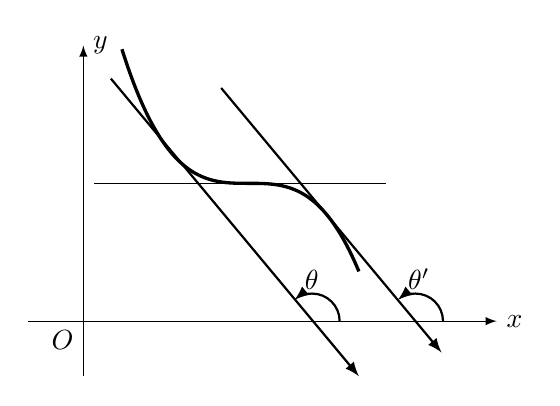
\begin{tikzpicture}[>=latex, scale=.7]
  \draw[->](-1,0)--(7.5,0)node[right]{$x$};
\draw[->](0,-1)--(0,5)node[right]{$y$};
\node at (0,0)[below left]{$O$};
\draw[domain=.7:5, samples=100, very thick]plot(\x, {-.2*(\x-3)^3+2.5});
\draw[->, domain=2.5:6.5, thick, samples=10]plot(\x, {-1.2*\x+7.23});
\draw[->, domain=.5:5, thick, samples=10]plot(\x, {-1.2*\x+5});
\draw(.2,2.5)--(5.5,2.5);
\draw[->, thick](6.025+.5,0) arc (0:129.8:.5)node[above right]{$\theta'$};
\draw[->, thick](4.15+.5,0) arc (0:129.8:.5)node[above right]{$\theta$};


    \end{tikzpicture}
    \caption{}
    \end{minipage}
  \end{figure}



\begin{example}
证明$\tan x>x,\quad 0<x<\frac{\pi}{2}$
\end{example}


\begin{proof}
我们只须证明$\tan x-x>0,\; 0<x<\frac{\pi}{2}$.为此,设$f(x)=\tan x-x,\; x\in\left(0,\frac{\pi}{2}\right)$,因为$f(x)$在$\left[0,\frac{\pi}{2}\right)$
上连续,且在$\left(0,\frac{\pi}{2}\right)$内$f'(x)=\sec^2x-1=\tan^2 x>0$,依定理2, $f(x)$在$\left[0,\frac{\pi}{2}\right)$上递增,所以有
\[f (x) > f (0) =\tan 0-0=0,\quad x\in \left(0,\frac{\pi}{2}\right)\]
即:$\tan x-x>0$,
也就是$\tan x>x,\quad 0<x<\frac{\pi}{2}$.
\end{proof}

\begin{example}
        求证当$x>0$时,有
$e^x> 1+\ln (1+x) $.
\end{example}


\begin{proof}
设$f(x)=e^x-1-\ln(1+x)\; (x>0)$, 则
\[f' (x) =e^x-\frac{1}{1+x},\qquad 
f''(x) =e^x +\frac{1}{(1+x)^2}\] 
    显然,当$x>0$时,$f''(x)>0$, 又$f'(x)$在$[0,\infty)$上连续,由定理2, $f'(x)$在$[0,\infty)$上递增,所以
\[f' (x) > f' (0) =e^0-\frac{1}{1+0}=0\quad  (x> 0) \]
又$f(x)$在$[0, \infty)$连续,同理$f(x)$在$[0, \infty)$上递增,所以当$x>0$时,有
\[f (x) > f (0) =e^0-1-\ln (1+0) =0\]
即:
\[e^x-1-\ln(1+x)>0\quad \text{或}\quad e^x>1+\ln(1+x)\]
\end{proof}


\begin{example}
    确定$f(x)=2x^3-9x^2+12x+5$的递增区间和递减区间,并画出这个函数图象的草图.
\end{example}


\begin{solution}
  \[  f'(x)=6x^2-18x+12=6(x-1)(x-2)\]

  当$x<1$或$x>2$时,$f'(x)>0$, 所以$f(x)$在区间$(-\infty,1)$和$(2,+\infty)$内递增;

  当$1<x<2$时,$f'(x)<0$,所以$f(x)$在区间$(1,2)$内递减.
  
  图象的$y$截距$f(0)=5$,为确定图象的$x$截距,根据例2.54和连续函数中间值定理,由计算的结果
  \[f(-1)=-18,\quad f(1)=10,\quad f(2)=9,\quad f(+\infty)>0\]
  得知$f(x)$在$(1, 2)$和$(2,+\infty)$内没有零点,即图象在$x>1$的范围内与$x$轴不相交:由于$f(x)$在$x<1$的区间内递增,并且$f(-1)\cdot f(0)<0$, 故$f(x)$的图象在
  $x<1$的范围内与$x$轴只有一个交点,它的横坐标在区间$(-1,0)$内.

  把$f(x)$的递增、递减情况列成下表,就更加醒目.

  \begin{center}
\begin{tabular}{c|ccccc}
\hline
$x$ & $(-\infty,1)$& 1& $(1,2)$ & 2& $(2,+\infty)$\\
\hline
$f'(x)$ & $+$ &0&$-$&0&$+$\\
$f(x)$ & $\nearrow$ &10&$\searrow$ &9&$\nearrow$ \\
\hline
\end{tabular}
  \end{center}
图象的草图如图2.27.

\begin{figure}[htp]
    \centering
\begin{tikzpicture}[>=latex, yscale=.3]
\draw[->](-2,0)--(4,0)node[right]{$x$};
\draw[->](0,-2)--(0,15)node[right]{$y$};
\draw[domain=-1:3, samples=300, very thick]plot(\x, {2*\x^3-9*\x^2+12*\x+5});
\draw[dashed](1,0)node[below]{1}--(1,10);
\draw[dashed](2,0)node[below]{2}--(2,9);
\draw(-1,0)node[below]{$-1$}--(-1,.2);
\end{tikzpicture}
    \caption{}
\end{figure}
\end{solution}

\begin{ex}
\begin{enumerate}
    \item     若$|f(x)-f(y)|\le (x-y)^n,\; n>1$,
   求证$f$是一常数.
    \item 若$f'(x)=g'(x)$, $x\in(-\infty,+\infty)$, 求证$f(x)=g (x) +c$.
    \item 证明在任何区间内,函数$x-\sin x$是增函数,又$\alpha$为何
    值,函数$\alpha x-\sin x$是增函数,$\alpha x-\sin x$为减函数?
    \item 证明$\frac{x}{\sin x}$在$\left(0,\frac{\pi}{2}\right]$内是增函数.
    \item 若$x>0$, 求证
\begin{multicols}{2}
  \begin{enumerate}
\item  $\cos x-1+\frac{1}{2}x^2> 0$
\item $\sin x-x+\frac{1}{6}x^3> 0$
\item  $x-\frac{x^2}{2}<\ln (1+x)<x$
\end{enumerate}  
\end{multicols}

\item 证明下列不等式当$0<x<\frac{\pi}{2}$时成立:
\begin{multicols}{2}
    \begin{enumerate}
        \item $\tan x> x+\frac{x^3}{3}$
        \item $\frac{\sin x}{x}> \frac{2}{\pi}$
    \end{enumerate}
\end{multicols}

\item 已知$x+e^x=y+e^y$, 问$\sin x=\sin y$是否为真?
\item 若$a>b$, 求证$a^3-3a^2+3a>b^3-3b^2+3b$.
\item 设$f(0)=0$, 且$f'$在$[0,+\infty)$内递增,证明
$ g(x) =\frac{f (x)}{x}$在$(0,+\infty)$内递增.
\item 
\begin{enumerate}
    \item 已知$a,b$为实数,并且$e<a<b$,其中$e$是自然对数的底,证明:$a^b>b^a$.
    \item 如果正实数$a,b$满足$a^b=b^a$, 且$a<1$, 则$a=b$.
\end{enumerate}

\item 证明:对于所有$x\in\left(0,\frac{\pi}{2}\right]$, 有不等式
$(\sin x)^{-2}\le x^{-2}+1-\frac{4}{\pi^2}$
成立.
\end{enumerate}
\end{ex}


\subsubsection{函数的极大值与极小值}

从例2.59我们看到$x=1$和$x=9$分别是函数$f(x)=2x^3-9x^2+12x+5$取到极大值$f(1)=10$和极小值$f(2)=9$的点,我们称$x=1$为极大点,$x=9$为极小点,以后,极大值与极小值统称为\textbf{极值},极大点与极小点统称为\textbf{极值点}.

下面我们来讨论如何确定一个函数的极值.
\begin{enumerate}
    \item 若$x_0$是$f(x)$的极值点,且$f(x)$在点$x_0$可微,那么总存在$x_0$的一个邻域,使$f(x)$在点$x_0$的邻域中满足费马条件,因而必有$f'(x_0)=0$. 例如例2.59, $f'(1)=f' (2) =0$.
    \item 若$f(x)$在$x_0$不可微,这时$x_0$也可能是极值点,例如,$f(x)=|x|$, 它在$x_0=0$这一点不可微,但从图2.28即可看出$x_0=0$是它的极小点.
\end{enumerate}

\begin{figure}[htp]
    \centering
    \begin{minipage}[t]{0.48\textwidth}
    \centering
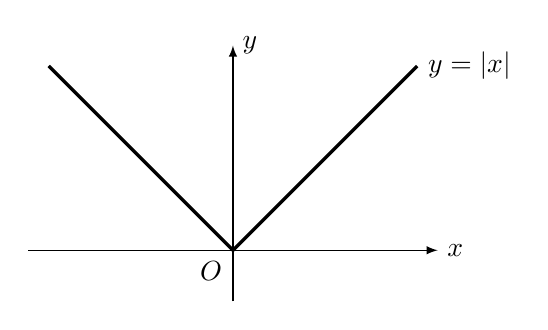
\begin{tikzpicture}[>=latex, scale=1.3]
    \draw[->](-2,0)--(2,0)node[right]{$x$};
\draw[->](0,-.5)--(0,2)node[right]{$y$};
\draw[very thick](-1.8,1.8)--(0,0)node[below left]{$O$}--(1.8,1.8)node[right]{$y=|x|$};
\end{tikzpicture}
    \caption{}
    \end{minipage}
    \begin{minipage}[t]{0.48\textwidth}
    \centering
    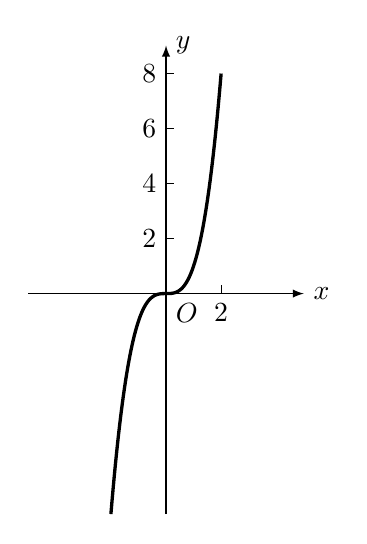
\begin{tikzpicture}[>=latex, scale=.35]
        \draw[->](-5,0)--(5,0)node[right]{$x$};
\draw[->](0,-8)--(0,9)node[right]{$y$};
\draw[domain=-2:2, samples=100, very thick]plot(\x, {\x^3});
\node at (0,0)[below right]{$O$};
\foreach \x in {2,4,6,8}
{
    \draw(0,\x)node[left]{$\x$}--(.3,\x);
}
\draw(2,0)node[below]{2}--(2,.3);
    \end{tikzpicture}
    \caption{}
    \end{minipage}
    \end{figure}


这就告诉我们连续函数的极值点应该从它的导函数$f'(x)$的零点和$f(x)$的不可微点中去找,但是,$f'(x)$的零点和$f(x)$的不可微点只是$f(x)$可能达到极值的点,并不一定是极值点,例如$f(x)=x^3$, $x=0$是$f'(x)=3x^2$的零点,然而在整个区间$(-\infty,+\infty)$上,$f'(x)\ge 0$, 而且只在$x=0$时,$f'(x)=0$, 即函数$f(x)=x$在$(-\infty,+\infty)$上严格递增,因而$x=0$不是极值点,它的图象如图2.29, 在$y$轴的左侧,图象位于切线$y=0$的下方;而在$y$轴的右侧,图象位于切线$y=0$的上方,我们把方程$f'(x)=0$的根称为函数$f(x)$的\textbf{驻点}.

又如函数
\[g(x)=\begin{cases}
    \frac{1}{2}(x-1), & x\in[1,2]\\
    \frac{3}{2}(x-2)+ \frac{1}{2}(2-1), & x\in[2,3]\\
 (x-3) +\frac{1}{2}(2-1) + \frac{3}{2}(3-2), & x\in[3,4]
\end{cases}\]
的图象是折线,如图2.30, 易知
\[g' (x) > 0,\quad x\in (1, 2) \cup (2, 3) \cup (3, 4) \]
但$g'(2)$和$g'(3)$不存在,由于$g(x)$在$[1, 4]$上严格递增,所以$x=2$, $x=3$都不是极值点.

\begin{figure}[htp]
    \centering
\begin{tikzpicture}[>=latex]
    \draw[->](-.5,0)--(5,0)node[right]{$x$};
    \draw[->](0,-.5)--(0,4)node[right]{$y$};
\draw[domain=1:2, samples=5, very thick]plot(\x, {.5*(\x-1)});
\draw[domain=2:3, samples=5, very thick]plot(\x, {1.5*(\x-2)+.5});
\draw[domain=3:4, samples=5, very thick]plot(\x, {(\x-3)+2});
\foreach \x in {1,2,3,4}
{
    \node at (\x,0)[below]{$\x$};
}
\draw[dashed](2,0)--(2,.5);
\draw[dashed](3,0)--(3,2)node[above left]{$y=g(x)$};
\draw[dashed](4,0)--(4,3);
\node at (0,0)[below left]{$O$};
\end{tikzpicture}
    \caption{}
\end{figure}

综上讨论,我们得到函数$f$取极值的必要条件:

\begin{blk}
    {定理1(极值的必要条件)}若$f(x)$在$[a,b]$上连续,$x_0$是$f(x)$的极值点,那么$x_0$只可能是$f'(x)$的零点或$f(x)$的不可微点.
\end{blk}

下面给出极值点的两个充分性判别法.

\begin{blk}
  {定理2} 如果函数$f$在$x_0$的邻域内连续,并且在$(x_0-\delta,x_0)$和$(x_0,x_0+\delta)\; (\delta>0)$可微:
\begin{itemize}
    \item 在$(x_0-\delta,x_0)$内,$f'(x)<0\; (>0)$;
    \item 在$(x_0,x_0+\delta)$内,$f'(x)>0\; (<0)$;
\end{itemize}
那么,$x_0$是$f$的局部极小点(极大点).
\end{blk}

\begin{proof}
按照前一节中定理2, $f$在$(x_0-\delta,x_0)$内严格递减(递增),而在$(x_0,x_0+\delta)$内严格递增(递减),故$f(x_0)$必为极小值(极大值).
\end{proof}

\begin{rmk}
    这个定理并不要求函数$f$在点$x_0$处存在导数,如果导数存在,那么根据费马定理,它等于零.
\end{rmk}


\begin{example}
    讨论$y=\sqrt[3]{(x-1)(x+2)^2}$的极值,并绘出图象的草图.
\end{example}

\begin{solution}
将$y=\sqrt[3]{(x-1)(x+2)^2}$的两边立方,得
\begin{align*}
    y^3&= (x-1) (x+2)^2\\
    3y^2\cdot y'&= (x+2)^2+ (x-1)\cdot 2\cdot  (x+2)\\
    &= (x+2) [x+2+2(x-1)]\\
    &=3x (x+2) 
\end{align*}

$\therefore\quad 
y'=\frac{x (x+2)}{y^2}=\frac{x (x+2)}{\sqrt[3]{(x-1)^2(x+2)^4}}$
即
\[y'=\frac{x}{\sqrt[3]{(x-1)^2(x+2)}}\quad 
(x\ne 1,\; x\ne -2)\]
\begin{itemize}
    \item 当$x=0$时,$y'=0$, 函数图象在点$x=0$处有水平切线;
    \item 当$x=-2$和1时,$y'$不存在,但是由$\Lim_{x\to 1}y'=+\infty$和$\Lim_{x\to -2^+}y'=-\infty$, 而$\Lim_{x\to -2^-}y'=+\infty$得知函数图象在点$x=1$和$x=-2$处有平行$y$轴的切线,所以函数的可能的极值点是$x=-2, 0, 1$这三个点.
\end{itemize}

为确定曲线的$y$截距,令$x=0$, 得$y=-\sqrt[3]{4}4\approx -1.59$; 为确定它的$x$截距,令$y=0$, 得$x=-2$和$x=1$, 现列表讨论它的增减性与极值如下:
\begin{center}
\begin{tabular}{c|ccccccc}
\hline
$x$ &$(-\infty,-2)$ & $-2$ & $(-2,0)$ & 0&$(0,1)$& 1& $(1,+\infty)$\\
\hline
$y'$ & $+$ & 不存在 & $-$ &0&$+$&不存在&$+$\\
$y$ & $\nearrow$ &极大值&$\searrow$ &极小值&$\nearrow$ &0&$\nearrow$\\ 
&&&0&&$-\sqrt[3]{4}\approx -1.59$\\
\hline
\end{tabular}
\end{center}

函数$y=\sqrt[3]{(x-1)(x+2)^2}$的图象如图2.31.
\begin{figure}[htp]
    \centering
\begin{tikzpicture}[>=latex]
    \draw[->](-4,0)--(3,0)node[right]{$x$};
    \draw[->](0,-3)--(0,3)node[right]{$y$};
\draw[domain=-4:-2.001, samples=100, very thick]plot(\x, {-exp(1/3*ln(1-\x)+2/3*ln(-\x-2))});

\draw[domain=-1.999:.999, samples=100, very thick]plot(\x, {-exp(1/3*ln(1-\x)+2/3*ln(\x+2))});
\draw[domain=1.001:2.25, samples=100, very thick]plot(\x, {exp(1/3*ln(\x-1)+2/3*ln(\x+2))});
\draw[very thick](1,.4)--(1,-.4);

\node at (-2,0) [above]{$-2$};
\node at (1,0) [below right]{$1$};
\draw(2,0)node[below]{$2$}--(2,.1);
\draw(-3,0)node[below]{$-3$}--(-3,.1);
\draw(-1,0)node[below]{$-1$}--(-1,.1);
\draw[dashed](-2,-3)--(-2,3);
\draw[dashed](1,-3)--(1,3);
\end{tikzpicture}
    \caption{}
\end{figure}
\end{solution}

\begin{blk}
{定理3} 设函数$f(x)$在区间$(a,b)$中有二阶连续的导函数,又$c\in (a,b)$, 使得$f' (c) =0$,
\begin{enumerate}
    \item 如果$f''(c)<0$, 则$c$是$f(x)$的一个极大点.
    \item 如果$f''(c)>0$, 则$c$是$f(x)$的一个极小点.
\end{enumerate}
\end{blk}

\begin{proof}
设$f''(c)<0$, 由于$f''(x)$的连续性,故存在点$c$的一个$\delta>0$的邻域$(c-\delta,c+\delta)\subset (a,b)$, 使得$f''(x)<0$, $x\in (c-\delta,c+\delta)$. 按前节定理2, $f'(x)$在$(c-\delta,c+\delta)$中是递减的,又由于$f'(c)=0$, 因此,
$f'(x)$在点$c$处由正变为负,由前面的定理2, $c$是$f(x)$的极大点.

当$f''(c)>0$时,同理可证$c$是$f(x)$的一个极小点.

为说明定理3的应用,我们求例2.60的二阶导函数:
\begin{align*}
   y''&=\frac{y^2 (2x+2) -x (x+2) \cdot 2y\cdot y'}{y^4}\\
&=\frac{2 [ (x+1) y-x (x+2) y']}{y^3} 
\end{align*}

从例2.60知,当$x=0$时,$y'=0$. 又$f(a)=-\sqrt[3]{4}$. 故在$x=0$处
\[y''_{x=0}=\frac{2\left[(0+1)\left(-\sqrt[3]{4}\right)-0\right]}{-4}=\frac{\sqrt[3]{4}}{2}>0\]
由定理3, $x=0$是函数$y=\sqrt[3]{(x-1)(x+2)^2}$的极小点.
\end{proof}




\begin{example}
    讨论$y=x^3+ax^2+bx+c$的极值.
\end{example}


\begin{solution}
\[y=x^3+ax^2+bx+c,\qquad 
    y'=3x^2+2ax+b\]

$ \Delta=a^2-3b$是导函数的判别式.
    我们可以分$\Delta>0$, $\Delta=0$和$\Delta<0$的三种情形讨论$y'$的正负区间.
\begin{enumerate}
    \item 若$\Delta>0$, 则
\[    y'=3x^2+2ax+b=3 (x-x_1) (x-x_2)\]
    这里$x_1=\frac{1}{3}\left(-a-\sqrt{a^2-3b}\right)$和$x_2=\frac{1}{3}\left(-a+\sqrt{a^2-3b}\right)$
    是导函数$y'$的二个实根.
\begin{enumerate}
    \item 当$x\in (-\infty,x)\cup (x_2,+\infty)$时,$y'>0$;
    \item 当$x\in (x_1,x_2)$时,$y'<0$
\end{enumerate}
    所以,$x_1$是$y$的一个极大点,$x_2$是$y$的一个极小点.
    
\item 若$\Delta=0$, 则
    \[y'=3x^2+2ax+\frac{a^2}{3}=3\left(x+\frac{a}{3}\right)^2\]
这里,$y'$虽然在$-\frac{a}{3}$处等于0, 但$y'$在$-\frac{a}{3}$的左、右两侧都取正值,即$y=x^3+ax^2+bx+c$是一个递增函数.因此,$-\frac{a}{3}$不是$y$的极值点.
\item 若$\Delta<0$, 则对于任意$x\in\mathbb{R}$, 恒有\[y'=3x^2+2ax+b=3 \left(x+\frac{a}{3}\right)^2+\frac{3b-a^2}{3}> 0\]
因此,$y=x^3+ax^2+bx+c$是一个增函数,也是没有极值点.
\end{enumerate}    
\end{solution}

\begin{ex}
\begin{enumerate}
    \item 先求出$f'(x)$, 然后由$f'(x)$的正负去讨论$f(x)$的增减与极值,并画出函数图象的草图:
\begin{multicols}{2}
    \begin{enumerate}
        \item $f (x) =2x^3+9x^2-24x+5$
        \item $f (x) =x^4-6x^2-8x+15$
        \item $f (x) =-x^5-5x^4$
        \item $f (x) = (x-1)^3$
     \item  $f (x) =|x^2-1|$
     \item $f (x) = (x^2-1)^3+1$
    \end{enumerate}
\end{multicols}
\item 讨论$f(x)=\frac{x^2-2x-3}{x^2+1}$的增减和极值,并画函数图象的草图.
    \item 求$f(\theta)=\sin\theta-\frac{1}{2}\sin2\theta$在$(-\pi,\pi)$内的极大值和极
    小值.
    \item 
\begin{enumerate}
    \item 求两条曲线$y=\frac{4e^x+2e^{-x}}{3}$和$y=e^{-x}$的交点的坐标;
    \item 求函数$y=\frac{4e^x+2e^{-x}}{3}$的极值点,又它在此点取极大值,还是极小值?
\end{enumerate}

\item 讨论函数$y=x^2e^{-x^2}$的增减与极值.
\item 求$f(x)=x^x\; (x>0)$的极值,并说明此极值是极大值
还是极小值.
\item 求函数$\frac{\ln x}{x}$的极大值,

\item 函数$f(x)=\frac{ax+b}{(x-1)(x-4)}$在点$(2,-1)$有一极值,
求$a,b$并证明此极值是极大值.
\item 证明$f(x)=\left(\alpha-\frac{1}{\alpha}-x\right)(4-3x^2)$仅有一个极大值
和一个极小值,且它们的差是$\frac{4}{9}\left(\alpha+\frac{1}{\alpha}\right)^3$, 又此差值的绝对值的最小值是多少?
\item 函数$f(x)=x(x-1)(x-a)$有绝对值相等,符号相反的
极大值与极小值,试确定常数$a$的值.
\item 求曲线$y=e^{-x}\sin x$上的极值点,并证明极值点上的纵坐
标成等比数列,又该等比数列的公比是多少?  
\end{enumerate} 
\end{ex}


\subsubsection{函数的最大值和最小值}
在实践中有一类“最大”、“最小”、“最省”的问题,例如生产搪瓷杯时,就要考虑在一定容积下,杯子的高和直径取多大时,用料最省.又如把一根圆木锯成矩形截面横梁时,怎样选取矩形的长和宽才能使横梁强度最大?这类“最大”、“最小”、“最省”等问题,在数学上叫做最大值、最小值问题.

我们曾在第一章中指出过“在闭区间$[a,b]$上连续的函数$f(x)$总是具有最大值和最小值”,但是,微积分并未提供确定函数$f(x)$的最大值、最小值的直接方法.如果我们讨论的函数$f(x)$在$(a,b)$上有连续的一阶导数,那么只要求出$f(x)$在$(a,b)$内的驻点,即$f'(x)=0$的根,就可以求出$f(x)$的局部极值.显然,$f(x)$在$[a,b]$上的最大值和最小值一定出现在局部极大值、局部极小值和端点值之中,从几何上来说,最大值、最小值如果不是位于定义区间的端点上,则分别是曲线的波峰和波谷.从图2.33可以看到局部极大值可能小于局部极小值.

\begin{figure}[htp]
    \centering
\begin{tikzpicture}[>=latex]
        \draw[->](-.5,0)--(5,0)node[right]{$x$};
        \draw[->](0,-.5)--(0,4.5)node[right]{$y$};
        
        \node at (0,0);
        \draw plot[smooth] coordinates{(.5,4)(1,2.5)(1.9, 3.5)(3.2, .8)(4,1.5)(4.4,1)};
%        \pscurve[linewidth=2pt](.5,4)(1,2.5)(1.9, 3.5)(3.2, .8)(4,1.5)(4.4,1)
%        };
        \draw[dashed](.5,4)--(.5,0)node[below]{$a$};
        \draw[dashed](4.4,1)--(4.4,0)node[below]{$b$};
\end{tikzpicture}
    \caption{}
\end{figure}

下面给出求函数$f(x)$在$[a,b]$上最大值和最小值的法则,这个法则适用于在$[a,b]$上连续,在$(a,b)$内可
微的函数$f(x)$,并且$f'(x)$最多在有限个点上等于零.
\begin{enumerate}
    \item 求$f(x)$在$(a,b)$内的驻点,即解$f'(x)=0$;
    \item 计算$f(x)$在驻点和端点的函数值,并把这些值加以比较,其中最大的一个为最大值,最小的一个为最小值.
\end{enumerate}

假如$f'(x)$在$(a,b)$内有一个驻点$c$, 且在整个$(a,b)$
上,$f''(x)<0\; (>0)$, 那么点$c$是最大值(最小值)点.

事实上,如果$f''(x)<0,\; x\in (a,b)$, 那么函数$f'(x)$在$[a,b]$上递减,因而$c$是其唯一的驻点,由中值定理知:

当$a\le x<c$时,$f'(x)-f'(c)=(x-c)\cdot f''(\xi)$,这里$x<\xi<c$.

$\because\quad f' (c) =0,\quad f'' (\xi)<0,\quad x-c<0$,

$\therefore\quad f'(x)>0$

同理说明当$c<x\le b$时,$f'(x)<0$.再根据$f(x)$在$[a,c]$上递增而在$[c,b]$上递减.故当$x\ne c$时有$f(x)<f(c)$.由此可知$c$是最大值点.当$f''(x)<0$时,也可以进行同样的论证.

如果$f(x)$在$[a,b]$内有不可微的点,而且这种点只有有限个,那么求最大值和最小值的法则改为求出三种点的对应函数值再加以比较,即$f(x)$的驻点的函数值,$f(x)$的不可微点的函数值,最后还有端点的函数值$f(a)$和$f(b)$, 这些值中最大的就是最大值,最小的就是最小值.

在实际问题中,如果在$(a,b)$内部,$f(x)$只有一个驻点$c$, 而且从实际问题本身又可以知道在$(a,b)$内必定有最大值或最小值,那么$f(c)$就是所要求的最大值或最小值,不需要算出$f(a)$, $f(b)$了.

\begin{example}
求函数$f(x)=x^{\tfrac{2}{3}}-(x^2-1)^{\tfrac{1}{3}}$在区间$[-2,2]$上的最大值和最小值.
\end{example}


\begin{solution}
\begin{align*}
f'(x)&=\frac{2}{3}x^{-\tfrac{1}{3}}-\frac{1}{3}(x^2-1)^{-\tfrac{2}{3}}\cdot 2x\\
&=\frac{2}{3} \frac{(x^2-1)^{\tfrac{2}{3}}-x^{\tfrac{4}{3}}}{x^{\tfrac{1}{3}}(x^2-1)^{\tfrac{2}{3}}}    
\end{align*}
    故$f(x)$的驻点是$\pm\frac{1}{\sqrt{2}}$, 不可微点是$x=0$, $x=\pm 1$, 且这些点都在$[-2, 2]$内,因此$f(x)$的极值点可能是
\[-1,\quad \frac{-1}{\sqrt{2}},\quad  0,\quad \frac{1}{\sqrt{2}},\quad  1\]
    由于$f(x)$是偶函数,故仅需计算
\[    f (0) =1,\qquad f\left(\frac{1}{\sqrt{2}}\right) =4,\qquad f (1) =1\]
    又在端点$x=2$处的函数值$f(2)=\sqrt[3]{4}-\sqrt[3]{3}$, 把上面这些函数直相互比较,可见$f(x)$在$[-2, 2]$中的最大值为$\sqrt[3]{4}\approx 1.59$, 最小值为$\sqrt[3]{4}-\sqrt[3]{3}\approx 1.59-1. 44\approx 0.15$.
\end{solution}

\begin{example}
    设$a>0$, 证明
$    f (x) =\frac{1}{1+|x|}+\frac{1}{1+|x-a|}$
    的最大值是$\frac{2+a}{1+a}$.
\end{example}    

\begin{proof}
把$f(x)$写成分段函数
\[f(x)=\begin{cases}
    \frac{1}{1-x}+\frac{1}{1+a-x}, & x<0\\
    \frac{1}{1+x}+\frac{1}{1+a-x}, & 0\le x\le a\\
    \frac{1}{1+x}+\frac{1}{1+x-a}, & x>a
\end{cases}\]
于是
\[f‘(x)=\begin{cases}
    \frac{1}{(1-x)^2}+\frac{1}{(1+a-x)^2}, & x<0\\
    \frac{-1}{(1+x)^2}+\frac{1}{(1+a-x)^2}, & 0\le x\le a\\
    \frac{-1}{(1+x)^2}+\frac{1}{(1+x-a)^2}, & x>a
\end{cases}\]
因而$f(x)$在$(-\infty, 0]$上递增,而在$[a,+\infty)$上递减,由此得知$f(x)$在$[0,a]$上的最大值也就是在$\mathbb{R}$上的最大值.

设对于$(0,a)$内的$x$有$f'(x)=0$, 则
\[(1+x)^2- (1+a-x)^2=0\]
上式唯一解是$x=\frac{a}{2}$. 
因为$f\left(\frac{a}{2}\right)=\frac{4}{2+a}$, $f(0)=f(a)=\frac{2+a}{1+a}$,
并且
\[\frac{2+a}{1+a}-\frac{4}{2+a}= \frac{a^2+4a}{(1+a) (2+a)}>0\quad  (a>0)\]
所以$f(x)$的最大值是$\frac{2+a}{1+a}$.
\end{proof}

\begin{example}
    用铁皮做体积为$V$的圆柱形封闭容器,如何使材料最省?
\end{example}


\begin{solution}
\textbf{解法1:} 设圆柱形底面半径为$r$, 高为$h$, 于是需用材料即圆柱表面积
\[S=2\pi rh+2\pi r^2\]
但$V=\pi r^2h$为已知,因此,$h=\frac{V}{\pi r^2}$,
从而问题变为求函数$S(r)=\frac{2V}{r}+2\pi r^2\; (0<r<+\infty)$的最小值.

根据经验,当$r$很小时,$S$很大,又当$r$很大时,$S$也很大,因此在$(0,+\infty)$内必有$r$的一个值使$S$最小,即它是$S'(r)=0$的一个根,由
\[S' (r) =-\frac{2V}{r^2}+4\pi r=0\]
得唯一正根$r=\sqrt[3]{\frac{V}{2\pi}}$.
从这个实际问题知道,当$r=\sqrt[3]{\frac{V}{2\pi}}$
时,$S$为最小,这时相应的高为
\[h=\frac{V}{\pi r^2}=\frac{2\pi r^3}{\pi r^2}=2r=2\sqrt[3]{\frac{V}{2\pi}}\]
这说明圆柱的高和直径相等时,用料最省.

\textbf{解法2:}  我们可以不先将下面两个式子中的$h$消去,再求$\frac{\dd S}{\dd r}=0$的根
\begin{align}
    S&=2\pi r h+2\pi r^2\\
    \pi r^2 h&=V
\end{align}
而是保留辅助变量$h$,将
(2.27), (2.28)对$r$求导数,只须记着$V$是常量,$h$是$r$的函数,于是由$\frac{\dd S}{\dd r}=0$,得
\begin{equation}
    \frac{\dd S}{\dd r}=2\pi\left(h+r\frac{\dd h}{\dd r}+2r\right)=0
\end{equation}
由(2.28)得
\begin{equation}
    \pi\left(2rh+r^2\frac{\dd h}{\dd r}\right)=0
\end{equation}
由此得:
\[\frac{\dd h}{\dd r}=-\frac{2h}{r}\]
将它代入(2.29),得
\[2r\left[h+r\left(-\frac{2h}{r}\right)+2r\right]=0\]
所以:$2r=h$. 

同样地说明了圆柱的高和直经相等时,用料最省.
\end{solution}


\begin{example}
由半径为$\ell$的圆铁皮,剪去一个扇形,把剩下的部分围成一个圆锥形容器,为了使用所得圆锥容器有最大的容积,问剪去扇形的中心角应该多大?
\end{example}

\begin{figure}[htp]
    \centering
\begin{tikzpicture}[>=latex]
\begin{scope}[scale=1.5]
\draw[pattern=north east lines](0,0)--(-135:1.5) arc (-135:135:1.5)--(0,0);
\draw[<->](-135:.2) arc (-135:135:.2);
\node at (.5,0)[fill=white]{$x$};
\node at (1,1)[above right]{$x\ell=2\pi r$};
\tkzDefPoint(-30:1.5){A}
\tkzDefPoint(-30:2){B}
\tkzDrawCircle(B,A)
\draw[->](B)--node[above]{$r$}+(10:.5);
\draw[decorate,decoration={brace,mirror,raise=2pt}](135:1.5)--node[below left]{$\ell$}(0,0);


\end{scope}
\begin{scope}[xshift=7cm, scale=.7]
\draw[dashed](0,-2) ellipse [x radius=1.5cm, y radius=.5cm];
\draw[thick](-1.5,-2)--(0,3)--node[above right]{$\ell$}(1.5,-2);
\draw[dashed](0,3)--node[left]{$h$}(0,-2)--node[below]{$r$}(1.5,-2);
\draw[thick](1.5,-2) arc [start angle =0, end angle=-180, x radius=1.5cm, y radius=.5cm];
\end{scope}


\end{tikzpicture}
    \caption{}
\end{figure}


\begin{solution}
    设剪去扇形后,所剩材料的圆心角为$x$(弧度),扇形的弧长为$x\ell$, 由它围成一个圆锥,其底面半径为$r$, 母线长为$\ell$, 高为$h$, 如图2.34. 于是
\[r=\frac{\ell x}{2\pi}\]
圆锥高为
\[h=\sqrt{\ell^2-r^2}=\sqrt{\ell^2-\left(\frac{\ell x}{2\pi}\right)^2}=\frac{\ell }{2\pi}\sqrt{4\pi^2-x^2}\]
因此圆锥的体积为
\begin{align*}
    V&=\frac{1}{3}\pi r^2 h\\
    &=\frac{1}{3}\pi\left(\frac{\ell x}{2\pi}\right)^2\cdot \frac{\ell}{2\pi}\sqrt{4\pi^2-x^2}\\
    &=\frac{\ell^3 x^2}{24\pi^2}\sqrt{4\pi^2-x^2}\quad (0\le x\le 2\pi)
\end{align*}
由于$V(0)=0$, $V(2\pi)=0$, 故在$(0, 2\pi)$内必有一个值$x_0$使$V$的值最大,因而使$V'(x_0)=0$. 由于
\begin{align*}
    V'(x)&=\frac{\ell^3}{24\pi^2}\left[2x\sqrt{4\pi^2-x^2}+\frac{1}{2}x^2(4\pi^2-x^2)^{-\tfrac{1}{2}}\cdot (-2x)\right]\\
    &=\frac{\ell^3}{24\pi^2}\left(\frac{8\pi^2 x-3x^3}{\sqrt{4\pi^2-x^2}}\right)
\end{align*}
令$V'(x)=0$, 即$8\pi^2 x-3x^3=0$, 解得
\[x_1=0,\quad x_2=-2\pi\sqrt{\frac{2}{3}}, \quad x_3=2\pi\sqrt{\frac{2}{3}}\]
这里只有$x_3=2\pi\sqrt{\frac{2}{3}}\in (0, 2\pi)$, 故知$x=2\pi\sqrt{\frac{2}{3}}$是$V(x)$在$[0, 2\pi]$内的唯一的极大点,因而也是最大点.于是最后得到结论,剪去扇形的圆心角为
\[2\pi-2\pi\sqrt{\frac{2}{3}}=\frac{2}{3}\pi\left(3-\sqrt{6}\right)\; \text{(弧度)}\]
时,才能使所围成的容器有最大的容积.
\end{solution}

\begin{example}
    求证:若$p>q>1$,又$x\ge 0$且$x\ne 1$,则$\frac{x^p-1}{p}>\frac{x^q-1}{q}$.
\end{example}

\begin{proof}
设$f(x)=\frac{x^p-1}{p}-\frac{x^q-1}{q}\; (x\ge 0)$,则:
\[f'(x)=x^{p-1}-x^{q-1}=x^{p-1}\left(x^{p-q}-1\right)\quad (p>q>1)\]
    函数的增、减如下表所示:
\begin{center}
\begin{tabular}{c|cccc}
\hline
$x$&0&$(0,1)$&1& $(1,+\infty)$\\
\hline
$f'(x)$&0&$-$&0&$+$\\
$f''(x)$&$\frac{1}{q}-\frac{1}{p}$&$\searrow$&极小值0& $\nearrow$\\ 
\hline
    \end{tabular}
\end{center}

$\because\quad f(0)=\frac{1}{q}-\frac{1}{p}>0=f(1)$

$\therefore\quad f(1)=0$不仅是极小值也是最小值.于是:
\[f(x)=\frac{x^p-1}{p}-\frac{x^q-1}{q}\ge 0\quad (x\ge 0)\]
因为$x\ne 1$,所以
\[\frac{x^p-1}{p}>\frac{x^q-1}{q}\quad (x\ge 0,\; x\ne 1)\]
\end{proof}

\begin{example}
 (光的折射定律)设有两种介质,$X'X$是它们的交界线,光由一种介质中的某点$A$走向另一种介质中的某点$B$. 又设当光走过交界线$X'X$时,它的速度由$v_1$变成$v_2$. 依据物理学中的一个基本原理“光由$A$到达$B$时,所采取的途径要使用的时间为最小”,如果两种介质是均匀的(例如一为空气,一为水),那么$v_1,v_2$都是常数,从而光在这两种介质中所走的路径是两段直线$AP$, $PB$, $P$表示光达到交界线时与这条线的交点,如果$AB$不与$X'X$垂直,一般$APB$不是直线,我们来定出$AP$, $BP$与$X'X$的法线的夹角$\theta_1$和$\theta_2$的关系.
\end{example}

    \begin{figure}[htp]
    \centering
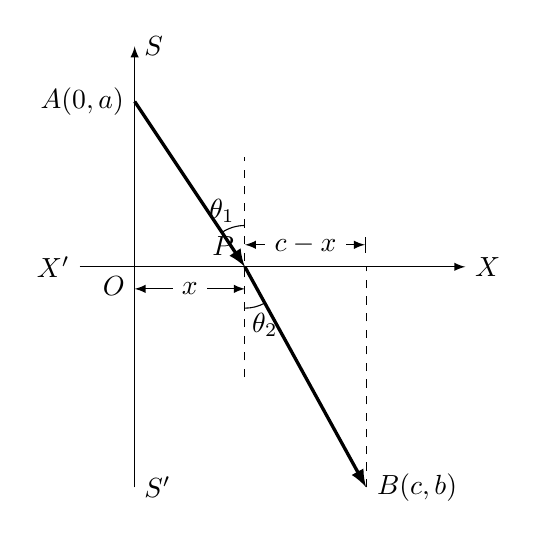
\begin{tikzpicture}[>=latex, scale=.7]
\draw[->](-1,0)node[left]{$X'$}--(6,0)node[right]{$X$};
\draw[->](0,-4)node[right]{$S'$}--(0,4)node[right]{$S$};
\node at (0,0)[below left]{$O$};
\draw[->, very thick](0,3)node[left]{$A(0,a)$}--(2,0)node[above left]{$P$};
\draw[->, very thick](2,0)--(4.2,-4)node[right]{$B(c,b)$};
\draw[dashed](2,-2)--(2,2);
\draw[<->](0,-.4)--node[fill=white]{$x$}(2,-.4);
\draw[|<->](4.2,.4)--node[fill=white]{$c-x$}(2,.4);
\draw[dashed](4.2,-4)--(4.2,0);
\draw(2,.75) arc (90:90+33.7:.75)node[above]{$\theta_1$};
\draw(2,-.75) arc (-90:-90+28.8:.75)node[below]{$\theta_2$};


\end{tikzpicture}
    \caption{}
\end{figure}

\begin{solution}
如图2.35建立坐标系,$A$点坐标是$(0,a)$, $B$点的坐标是$(c,b)$, 设$P$点的坐标是$(x,0)$, 光由$A$到$P$所需时间是$\frac{\sqrt{a^2+x^2}}{v_1}$,从$P$到$B$所需时间是$\frac{\sqrt{b^2+(c-x)^2}}{v_2}$, 
则整个时间$t(x)$是
\[t (x) =\frac{\sqrt{a^2+x^2}}{v_1}+\frac{\sqrt{b^2+(c-x)^2}}{v_2}\]

为了使$t(x)$极小,应使$t'(x)=0,\; x\in (0,c)$. 由$t(x)$得
\begin{align*}
    t' (x) &=\frac{x}{v_1\sqrt{a^2+x^2}}-\frac{c-x}{v_2\sqrt{b^2+(c-x)^2}}\\
    t'' (x) &=\frac{-x^2}{v_1(a^2+x^2)^{\tfrac{3}{2}}}+\frac{1}{v_1\sqrt{a^2+x^2}}+\frac{1}{v_2\sqrt{b^2+(c-x)^2}}-\frac{(c-x)^2}{v_2\left[b^2+(c-x)^2\right]^{\tfrac{3}{2}}}\\
    &=\frac{a^2}{v_1(a^2+x^2)^{\tfrac{3}{2}}}+\frac{b^2}{v_2\left[b^2+(c-x)^2\right]^{\tfrac{3}{2}}}>0.
\end{align*}
既然$t'(0)<0$, $t'(c)>0$, 及$t'$是严格递增的,故在$(0,c)$内有唯一的$x_0$, 使得
\[t'(x_0)=0\]
从而当$x=x_0$时,$t(x_0)$是极小值也是最小值,于是由$t'(x_0)=0$得到
\[\frac{x_0}{v_1\sqrt{a^2+x^2_0}}=\frac{c-x_0}{v_2\sqrt{b^2+(c-x_0)^2}}\]
即
\[\frac{\sin\theta_1}{v_1}=\frac{\sin\theta_2}{v_2}\]
这就是光的折射定律.
\end{solution}

\begin{ex}
\begin{enumerate}
    \item 由$y=0$, $x=8$, $y=x^2$围成一曲边三角形$OAB$, 在曲边$\wideparen{OB}$上,求一点使得过此点所作$y=x^2$的切线与$OA$、$AB$所围成的三角形面积最大.
    \item 椭圆$\frac{x^2}{a^2}+\frac{y^2}{b^2}=1$的内接矩形中怎样的矩形面积最大?又此最大的矩形面积比椭圆的内接正方形的面积大多少?
    \item 设$\triangle ABC$是定圆的内接三角形,其中$A$、$B$两点固定,$C$点在圆周上变动,试求其面积最大时的位置.
    \item 要做一个底面为长方形的带盖箱子,其体积为72立方厘米,其底边成$1:2$的关系,问各边的长怎样,才能使表面积最小?
    \item 设有底为等边三角形的直棱柱,体积为$V$, 要使其总面积为最小,问底边长应为多少?
    \item 设正三棱锥的侧面积为$S$, 问当侧面与底面所成角$\alpha$为何值时,其体积最大?
    \item 平面上通过一个已知点$P(1, 4)$引一条直线,要使它在两个坐标轴上的截距都为正,且它们的和为最小,求这条直线的方程.
    \item 直圆柱内接于半径为$R$的球中,当圆柱的高为何值时,其
    体积最大.
    \item 三个点$A$, $B$和$C$不在同一直线上,$\angle ABC=60^{\circ}$, 汽车以80公里/小时的速度由$A$向$B$行驶,同时火车以50公里/小时的速度由$B$向$C$行驶.若$AB=200$公里,问运动开始几小时后汽车与火车的距离最小?
    \item 船航行一昼夜的耗费由两部分组成:一为固定部分,设为$a$元;另一为变动部分,设它与速度立方成比例,试问船应以怎样的速度$v$行驶为最经济?
    \item 在某种产品的制造过程中,次品率$y$依赖于日产量$x$, 即$y=y(x)$, 已知
\[y(x)=\begin{cases}
    \frac{1}{101-x},& 0\le x\le 100,\\
    1,& x>100
\end{cases}\]
其中$x$为正整数.又该厂每生产一件产品可盈利$A$元,但每生产出一件次品就要损失$\frac{A}{3}$元.问为了获得最大盈利,该厂的日产量应定为多少?
\item 抛物线$y=x^2$上的哪一点到直线$x-y-2=0$的距离最短?\item 一弹在空中飞行(不计空气阻力),其弹道方程为
\[y=mx-\frac{(m^2+1)x^2}{800}\]
这里原点取在此弹发射之点,其中$m$为曲线在原点处的切线斜率.
\begin{enumerate}
    \item 若要此弹击中同一水平面上最远距离的目标;
    \item 若要此弹击中300米远处一直立墙壁上的最大高度,问$m$之值各为多少?
\end{enumerate}
\item 若直角三角形的周长$2p$一定,求它的面积的最大值.
\end{enumerate}  
\end{ex}

\subsection{函数的凸性与拐点}
上面已经讨论了函数的增减性与极值,这对于我们了解函数的性质与图象形状有很大的帮助.现在我们还要进一步考察函数在什么区间是向上凸的,什么区间是向下凸的,以及上凸函数和下凸函数的一些性质.

\begin{blk}
    {定义1} 函数$f$在区间$(a,b)$内,称为向下(上)凸的,指对于任意$c\in (a,b)$, 曲线位于在点$(c,f(c))$处的切线上(下)面(见图2.37和2.38).
\end{blk}    


\begin{figure}[htp]
    \centering
    \begin{minipage}[t]{0.48\textwidth}
    \centering
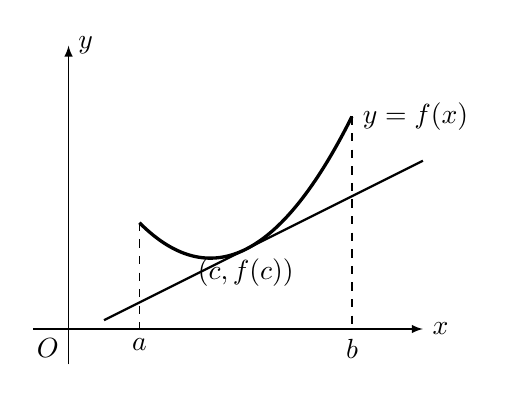
\begin{tikzpicture}[>=latex, scale=.9]
\draw[->](-.5,0)--(5,0)node[right]{$x$};
\draw[->](0,-.5)--(0,4)node[right]{$y$};
\draw[domain=1:4, samples=100, very thick]plot(\x,{0.5*(\x-2)^2+1})node[right]{$y=f(x)$};
\draw[dashed](1,1.5)--(1,0)node[below]{$a$};
\draw[dashed](4,3)--(4,0)node[below]{$b$};
\draw[domain=.5:5, samples=10,thick]plot(\x,{0.5*\x-0.125});
\node at (0,0)[below left]{$O$};
\node at (2.5,1.125)[below]{$(c,f(c))$};
\end{tikzpicture}
    \caption{}
    \end{minipage}
    \begin{minipage}[t]{0.48\textwidth}
    \centering
    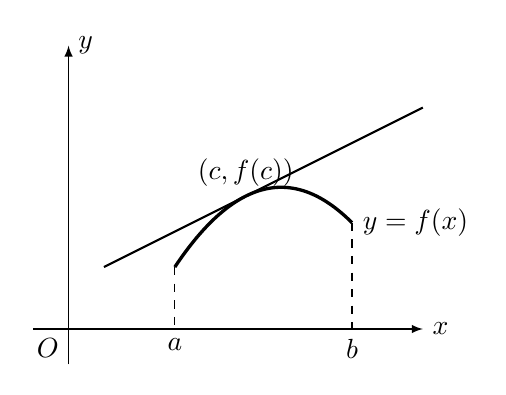
\begin{tikzpicture}[>=latex, scale=.9]
\draw[->](-.5,0)--(5,0)node[right]{$x$};
\draw[->](0,-.5)--(0,4)node[right]{$y$};
\draw[domain=1.5:4, samples=100, very thick]plot(\x,{-0.5*(\x-3)^2+2})node[right]{$y=f(x)$};
\draw[dashed](1.5,.875)--(1.5,0)node[below]{$a$};
\draw[dashed](4,1.5)--(4,0)node[below]{$b$};
\node at (2.5,1.875)[above]{$(c,f(c))$};
\draw[domain=.5:5, samples=10,thick]plot(\x,{0.5*\x+0.625});
\node at (0,0)[below left]{$O$};
    \end{tikzpicture}
    \caption{}
    \end{minipage}
    \end{figure}


\begin{blk}
    {定义2} 函数$f$的图象若经过某点$x=c$时,它的图象
$y=f(x)$由向上凸变为向下凸,或者由向下凸变为向上凸,则点$x=c$称为函数$f$的\textbf{拐点},如图2.39和2.40.
\end{blk}    
    

\begin{figure}[htp]
    \centering
    \begin{minipage}[t]{0.48\textwidth}
    \centering
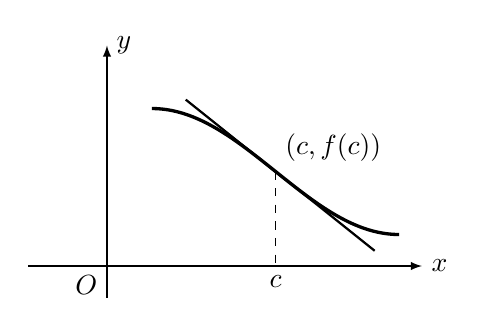
\begin{tikzpicture}[>=latex, yscale=.8]
    \draw[->](0,.5)--(5,.5)node[right]{$x$};
    \draw[->](1,0)--(1,4)node[right]{$y$};
    \draw[domain=.5*pi:1.5*pi, samples=100, very thick]plot(\x,{sin(\x r)+2});
    \node at (1,.5)[below left]{$O$};
\node at (3.1416, 2)[above right]{$(c,f(c))$};
\draw[domain=2:4.4, samples=10, thick]plot(\x,{-\x+5.1416});
\draw[dashed](3.1416,2)--(3.1416,.5)node[below]{$c$};
\end{tikzpicture}
    \caption{}
    \end{minipage}
    \begin{minipage}[t]{0.48\textwidth}
    \centering
    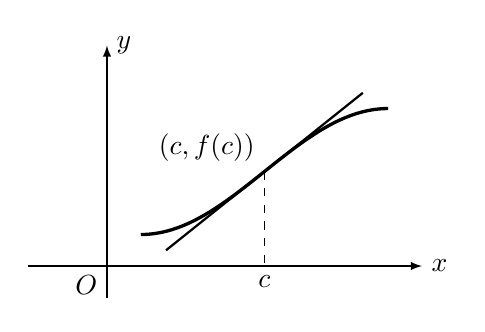
\begin{tikzpicture}[>=latex, yscale=.8]
   \draw[->](-3,.5)--(2,.5)node[right]{$x$};
    \draw[->](-2,0)--(-2,4)node[right]{$y$};
    \draw[domain=-.5*pi:.5*pi, samples=100, very thick]plot(\x,{sin(\x r)+2});
    \node at (-2,.5)[below left]{$O$};
\node at (0,2)[above left]{$(c,f(c))$};
\draw[domain=-1.25:1.25, samples=10, thick]plot(\x,{\x+2});   
\draw[dashed](0,2)--(0,.5)node[below]{$c$};

    \end{tikzpicture}
    \caption{}
    \end{minipage}
    \end{figure}


这时过$x=c$的点的切线,把曲线分成两部分,换言之,存在充分小的邻域$\delta>0$, 使得对于一切$x\in (c-\delta,c)$, 曲线位于在点$c$处的切线的一方,而对于$x\in (c,c+\delta)$, 曲线在该切线的另一方.

\begin{blk}
  {凸性判定定理} 设函数$f$在区间$(a,b)$内有二阶导数,则
\begin{enumerate}
    \item 函数f在区间$(a,b)$内为向下凸的充分必要条件是,对于每个$x\in (a,b)$, 有$f''(x)\ge 0$;
    \item 函数f在区间$(a,b)$内为向上凸的充分必要条件是,对于每个$x\in (a,b)$, 有$f''(x)\le 0$.
\end{enumerate}
\end{blk}

\begin{proof}
    假设曲线$y=f(x)$在$(a,b)$内是向下凸的,因为函数$f$在$(a,b)$内有二阶导数,则对于任意一点$c\in(a,b)$, $f'(c)$存在,曲线$y=f(x)$在点$x=c$处的切线方程是
\begin{equation}
    y=f (c) +f' (c) (x-c)
\end{equation}
    对于每个点$x\in (a,b)$, 曲线$y=f(x)$的对应点的纵坐
标与切线上的对应点的纵坐标之差用$g(x)$表示,如图2.41, 于是
\begin{equation}
   g (x) =f (x) -[f (c) +f' (c) (x-c)]=[f(x)-f (c) ] - (x-c) f' (c)  
\end{equation}
根据中值定理,得到
\[g (x) = (x-c) f' (d) - (x-c) f'(c)\]
这里$d\in (x,c)$或$(c,x)$. 又$g(x)=(x-c)\cdot [f'(d)-f'(c)]$, 再根据中值定理,得到
\begin{equation}
    g (x) = (x-c) (d-c)f''(e)
\end{equation}
这里$e\in (d,c)$或$(c,d)$.

于是对于一切$x\in (a,b)$, 点$(x,f(x))$不在切线(2.31)的下方的充要条件是$g(x)\ge 0$, 显然只有点$c$使$g(c)=0$. 根据等式(2.33), 并且注意到
\[(x-c)(d-c)>0\]
便知道$g(x)\ge 0$的充分必要条件是$f''(e)\ge 0$. 这里$e\in(a,b)$且随着$c$和$x$的不同值而改变.因此,依曲线向下凸的定义,曲线向下凸的充分必要条件是对于任意$x\in (a,b)$有$f''(x)\ge 0$.

用同样的方法便可说明曲线$y=f(x)$向上凸的充分必要条件是$f''(x)\le 0$.
\end{proof}

\begin{figure}[htp]
    \centering
    \begin{minipage}[t]{0.48\textwidth}
    \centering
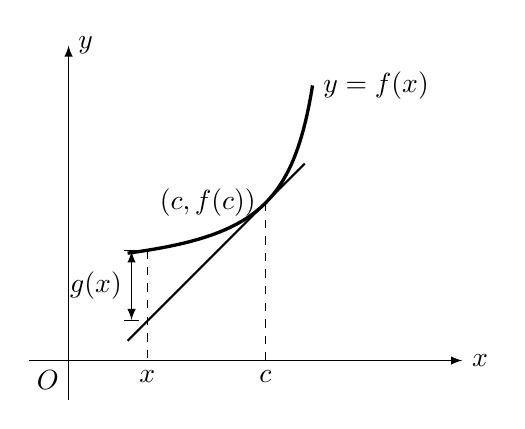
\begin{tikzpicture}[>=latex, scale=1]
    \draw[->](-.5,0)--(5,0)node[right]{$x$};
\draw[->](0,-.5)--(0,4)node[right]{$y$};
\draw[domain=.75:3.1, samples=100, very thick]plot(\x, {-1/(\x-3.5)+1})node[right]{$y=f(x)$};
\draw[domain=.75:3, samples=10, thick]plot(\x,{\x-0.5});
\draw[dashed] (2.5,2)node[left]{$(c,f(c))$}--(2.5,0)node[below]{$c$};
\draw[dashed] (1,1.4)--(1,0)node[below]{$x$};
\draw[|<->|](.8,1.4)--node[left]{$g(x)$}(.8,.5);
\node at (0,0) [below left]{$O$};
\end{tikzpicture}
    \caption{}
    \end{minipage}
    \begin{minipage}[t]{0.48\textwidth}
    \centering
    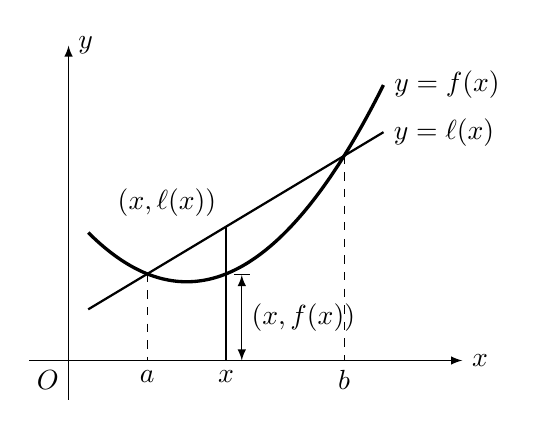
\begin{tikzpicture}[>=latex, scale=1]
       \draw[->](-.5,0)--(5,0)node[right]{$x$};
\draw[->](0,-.5)--(0,4)node[right]{$y$};
\draw[domain=.25:4, samples=100, very thick]plot(\x,{0.4*(\x-1.5)^2+1})node[right]{$y=f(x)$};
\draw[domain=.25:4, samples=10, thick]plot(\x,{.6*\x+.5})node[right]{$y=\ell(x)$};

\draw[dashed] (1,1.1)--(1,0)node[below]{$a$};
\draw[dashed] (3.5,2.6)--(3.5,0)node[below]{$b$};
\draw(2,0)node[below]{$x$}--(2,1.7)node[above left]{$(x,\ell(x))$};
\draw[<->|](2.2,0)--node[right]{$(x,f(x))$}(2.2,1.1);
\node at (0,0)[below left]{$O$};
    \end{tikzpicture}
    \caption{}
    \end{minipage}
    \end{figure}

向下凸或向上凸的函数的重要性质如下面的定理所述:

\begin{blk}
    {定理} 设$f$是$[a,b]$上二次可微函数,并且$f''(x)>0$, $x\in (a,b)$, 那么对于每一个满足$a<x<b$的$x$,有
\[f(x)<f(b)\cdot \frac{x-a}{b-a}+f(a)\cdot \frac{b-x}{b-a}\]
\end{blk}

这一定理有一个明显的几何意义(图2.42),用$\ell(x)$表示右端的一次函数:
\[\ell(x)=f(b)\cdot \frac{x-a}{b-a}+f(a)\cdot \frac{b-x}{b-a}\]
    它在$x=a$和$x=b$的值是$\ell(a)=f(a)$和$\ell(b)=f(b)$, 即与$f(x)$在这些点的值一致.因为$y=\ell(x)$的图象是$y=f(x)$在$[a,b]$上的割线,因此$[a,b]$上的向下凸函数$f$的图象$y=f(x)$位于该区间的割线的下面.





\begin{proof}
设$F(x)=f(x)-f(b)\frac{x-a}{b-a}-f(a)\frac{b-x}{b-a}$,
这里$x\in [a,b]$. 我们需要证明在$[a,b]$上,$F(x)\le 0$. 因为$F(x)$在$[a,b]$上连续,所以$F(x)$在$[a,b]$的某点达到它的最大值,用$c$表示最大值点,我们证明$c$是两端点之一.

假设$a<c<b$,那么$c$也是$F(x)$的极大值点.因此$F'(c)=0$. 又
\begin{align*}
    F'(x)&=f'(x)-\frac{f(b)}{b-a}+\frac{f(a)}{b-a}\\
    F''(x)&=f''(x)>0,\qquad x\in(a,b)
\end{align*}
因此我们得出结论,$F(c)$是$[a,b]$上的最小值,即对于
任意$x\in [a,b]$且$x\ne c$, 有
\[F (x) > F (c) =f (c) -\ell (c)\]
这与$c$是极大值点矛盾,因此,唯一的可能是$c$是一个端点$a$或$b$, 但是$f(a)=\ell(a)$, $f(b)=\ell(b)$, 这表明$F(x)=f(x)-\ell(x)$的最大值是0, 因此在$[a,b]$上除端点以外的所有其它点$x$, 有
\[F (x) =f (x) -f (b) \frac{x-a}{b-a}-f (a) \frac{b-x}{b-a}<0\]
即
\[f (x)<f (b) \frac{x-a}{b-a}+f (a) \frac{b-x}{b-a}\]
这就完成了向下凸函数定理的证明.
\end{proof}

对于向上凸函数有类似的定理,即:区间$[a,b]$上向上凸的函数的图象位于$[a,b]$的割线上面,用式子表示就是
\[f (x)>f (b) \frac{x-a}{b-a}+f (a) \frac{b-x}{b-a},\quad x\in(a,b)\]

\begin{example}
    求证 $\cos\pi x>1-2x,\quad x\in\left(0, \frac{1}{2}\right)$.
\end{example}


\begin{proof}
    设$f(x)=\cos\pi x$, $\ell (x)=1-2x$, 因为
\[f (0) =1=\ell (0) ,\qquad f \left(\frac{1}{2}\right) =0=\ell\left(\frac{1}{2}\right)\]
所以:$y=1-2x$是曲线$y=\cos\pi x$在$\left[0,\frac{1}{2}\right]$上的割线.

又$f'(x)=-\pi \sin\pi x$, $f''(x)=-\pi^2\cos\pi x$, 且当$x\in \left(0,\frac{1}{2}\right)$时,有$f''(x)<0$, 即$f(x)$在$\left(0,\frac{1}{2}\right)$内是向上凸
的.因此,$y=\cos\pi x$在$\left[0,\frac{1}{2}\right]$上的图象是在该区间的割
线$y=1-2x$的上面,从而
\[\cos\pi x>1-2x,\qquad x\in \left(0,\frac{1}{2}\right)\]
\end{proof}

下面给出拐点满足的必要条件.

\begin{blk}
    {定理} 如果$x=c$是曲线$y=f(x)$的拐点,并且$f''(c)$存在,则$f''(c)=0$.
\end{blk}

\begin{proof}
    因为$x=c$是曲线的拐点,即它是曲线$y=f(x)$向上凸和向下凸的分界点,依凸性判定定理,我们可以取$a<c<b$, 使得$f''(x)$在$(a,c)$内的函数值的符号与在$(c,b)$内的函数值的符号相反.

设$g(x)=f'(x),\; x\in (a,b)$, 于是$g'(x)=f''(x)$经过$c$点由负变正或由正变负,因此点$c$是$g(x)$在$(a,b)$内的唯一的极值点,又$g'(c)=f''(c)$存在,根据费马定理
\[g' (c) =f'' (c) =0\]
\end{proof}


\begin{example}
    讨论函数$f(x)=x^3$和$f(x)=x^4$有无拐点.
\end{example}


\begin{solution}
    $f(x)=x^3$有导数$f'(x)=3x^2$, $f''(x)=6x$, 显然$f'(0)=f''(0)=0$, 而且:
当$x>0$时,$f''(x)>0$; 当$x<0$时,$f''(x)<0$, 即曲线$y=x^3$在$(-\infty, 0)$内是向下凸的,而在$(0,+\infty)$区间内是向上凸的.因此,$x=0$是曲线的拐点而不是极值点.

又$f(x)=x^4$有导数$f'(x)=4x^3$, $f''(x)=12x^2$, 显然$f'(0)=f''(0)=0$, 并且对于每一个$x\ne 0$都有$f''(x)>0$, 因此这个曲线$y=x^4$是处处向下凸的,$x=0$不是曲线$y=x^4$的拐点而是一个极小点.
\end{solution}


下面给出判定拐点的充分条件.
    
\begin{blk}
   {定理(拐点的充分条件)} 设$f$在点$c$处连续,在点$c$附近(可以不包括$c$点)具有二阶导数,如果自变量$x$通过$c$时,二阶导数变号,则$x=c$是曲线$y=f(x)$的拐点.
\end{blk}

\begin{proof}
    我们可以取$c$点的一个邻域$(a,b)$使$f''(x)$在
$(a,c)$上的函数值的符号和在$(c,b)$上的相反,依凸性判定定理,$f$经过$c$时将由向上凸变为向下凸或者由向下凸变为向上凸,即$x=c$是曲线$y=f(x)$的拐点.
\end{proof}


\begin{example}
说明$x=0$是曲线$y=x^{\tfrac{1}{3}}$的拐点.
\end{example}

\begin{proof}
    设$f(x)=x^{\tfrac{1}{3}}$,则
\[f'(x)=\frac{1}{3x^{\tfrac{2}{3}}},\qquad f''(x)=\frac{-2}{9x^{\tfrac{5}{3}}}\]
显然$f'(0)$和$f''(0)$都不存在,但是当$x<0$时,$f''(x)>0$, 即曲线$y=x^{\tfrac{1}{3}}$向下凸;当$x>0$时,$f''(x)<0$, 即曲线$y=x^{\tfrac{1}{3}}$向上凸,因此点$x=0$是曲线的拐点.

由$\Lim_{x\to 0}f'(x)=\Lim_{x\to 0}\frac{1}{3x^{\tfrac{2}{3}}}=+\infty$知,曲线在点$x=0$处的切线就是$y$轴本身(见图2.43).
\end{proof}

\begin{figure}[htp]
    \centering
    \begin{minipage}[t]{0.48\textwidth}
    \centering
\begin{tikzpicture}[>=latex, scale=1]
    \draw[->](-2.5,0)--(2.5,0)node[right]{$x$};
\draw[->](0,-2)--(0,2)node[right]{$y$};
\draw[domain=-1.3:1.3, samples=100, very thick]plot({\x^3},\x)node[above]{$y=x^{\tfrac{1}{3}}$};
\node at (0,0) [above left]{$O$};
\end{tikzpicture}
    \caption{}
    \end{minipage}
    \begin{minipage}[t]{0.48\textwidth}
    \centering
    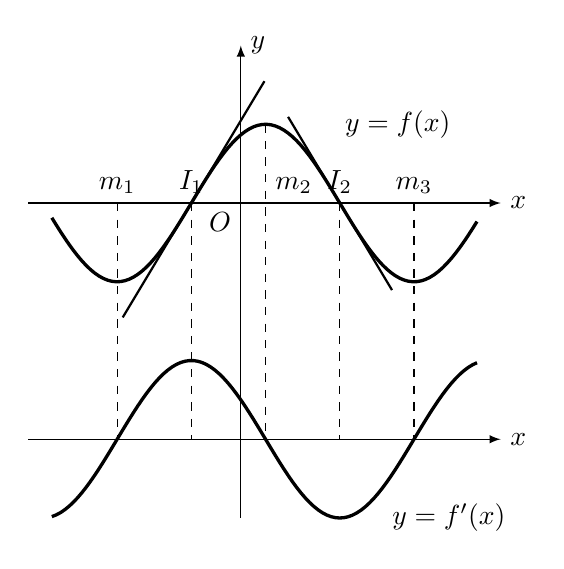
\begin{tikzpicture}[>=latex, xscale=.6]
       \draw[->](-4.5,0)--(5.5,0)node[right]{$x$};
\draw[->](0,-4)--(0,2)node[right]{$y$};
\draw[->](-4.5,-3)--(5.5,-3)node[right]{$x$};
\node at (0,0)[below left]{$O$};
\draw[domain=-4:5, samples=100, very thick]plot(\x, {sin((\x+pi/3)*180/pi)});
\draw[domain=-4:5, samples=100, very thick]plot(\x, {cos((\x+pi/3)*180/pi)-3});

\foreach \x/\xtext in {1.5*pi/m_3, -.5*pi/m_1, 0/I_1, pi/I_2}
{
   \draw[dashed](\x-pi/3, 0)node[above]{$\xtext$}--(\x-pi/3, -3);
}
\draw[dashed](.5*pi-pi/3, 1)--(.5*pi-pi/3, -3);
\node at (.5*pi-pi/3,0)[above right]{$m_2$};

\draw[domain=-2.5:.5, samples=10, thick]plot(\x, {\x+pi/3});
\draw[domain=1:3.2, samples=10, thick]plot(\x, {-\x+2*pi/3});
\node at (2,1)[right]{$y=f(x)$};
\node at (3,-4)[right]{$y=f'(x)$};
    \end{tikzpicture}
    \caption{}
    \end{minipage}
    \end{figure}

在图2.44中,函数$y=f(x)$的图象上的极值点$m_1$, $m_2$和$m_3$, 对应于函数$y=f'(x)$图象上的零点;$y=f(x)$的图象上的拐点对应于$y=f'(x)$的图象上的极值点.

\begin{ex}
\begin{enumerate}
    \item 讨论下列函数的极值、凸性及拐点,并出函数图象的
    草图;
\begin{multicols}{2}
\begin{enumerate}
    \item $f(x)=\frac{1}{1+x^2}$
    \item $y=(x-1)\sqrt[3]{x^2}$
\end{enumerate}
\end{multicols}
\item 如果函数$f(x)$在区间$(a,b)$内有二阶导数,并且向上凸,求证:对于满足条件$a\le x_1<x_2\le b$的任意两点$x_1,x_2$,恒有
\[f (\lambda x_1+ (1-\lambda) x_2) \ge \lambda f (x_1) + (1-\lambda)f (x_2) ,\quad  0\le\lambda\le 1\]
如果上面的函数在区间$(a,b)$内向下凸,则应有怎样的结论?
\item 求证函数
\begin{enumerate}
    \item $y=\log_ax \; (a>1)$在区间$(0,+\infty)$内是向上凸的;
    \item $f(x)=\sin x$在$[0,\pi]$内是向上凸的;
    \item $\log_a\frac{x_1+x_2}{2}\ge \frac{\log_a x_1+\log_a x_2}{2}\quad (x_1> 0,\; x_2>2)$
    \item $\sin\frac{x_1+x_2}{2}\ge \frac{\sin x_1+\sin x_2}{2}\quad  (0\le x_1,x_2\le \pi)$
\end{enumerate}

\item 如果函数$f(x)$在$(a,b)$内是向上凸的,求证:对于任意$a\le x_1<x_2<x_3\le b$,$\sum^3_{i=1}\lambda_i=1$,有
\[f(\lambda_1x_1+\lambda_2x_2+\lambda_3x_3)\ge \lambda_1f(x_1)+\lambda_2f(x_2)+\lambda_3f(x_3)\]

\item  求证对于任意正数$x_1,x_2,x_3$有
\[\ln\left(\frac{1}{6}x_1+\frac{1}{3}x_2+\frac{1}{2}x_3\right) \ge \ln \left(x_1^{\tfrac{1}{6}}x_2^{\tfrac{1}{3}}x_3^{\tfrac{1}{2}} \right)\]
\item  若$A,B,C$是任意三角形的三个内角,求证
\[\sin A+\sin B+\sin C\le \frac{3\sqrt{3}}{2}\]
又当$A,B,C$为何值时,上面等式成立?
\item  对于$a>0$, $b>0$, $0<\alpha<1$, $0<\beta<1$,$\alpha+\beta=1$,求证:
$a^{\alpha}b^{\beta}\le \alpha a+\beta b$成立.
(提示:利用对数函数是上凸函数)
\item  $f(x)=a_4x^4+a_3x^3+a_2x^2+a_1x+a_0$为具有正系数
的非零多项式,若为偶函数,求证$f(x)$在$(-\infty,+\infty)$内向下凸,且仅有一个极值.
\end{enumerate}
\end{ex}

\subsection{作函数的图象}
给出函数$y=f(x)$, 常常希望画出它的图象来,这对于许多问题是有用的,在初中我们所介绍的用列表法来描绘函数的图象,有很大的不精确性和盲目性,由于所取的点是有穷多个,很可能在所要画出的某两点之间的曲线有比较剧烈的变化,如果我们用比较平滑的曲线弧去连结,于是所得
曲线与实际相差很大.以前各节所介绍的函数性态可以帮助我们断定函数图象的主要特征,因此在取点之前,应先对函数的性态作一番讨论,兹将描绘曲线的一般步骤列出如下:

\begin{enumerate}
\item 确定函数的定义域;
\item 确定曲线关于坐标轴的对称性;
\item 确定曲线与坐标轴的交点(如果不易确定,不必强求);
\item 确定函数的增减性,极大值与极小值;
\item 确定函数的凸性与拐点;
\item 确定曲线的渐近线;
\item 需要时,还得由曲线方程计算出一些适当的点的坐标;
\item 把上面所得的结果,按自变量大小顺序列入一个表格内,以观察图形的大概形态,然后描绘成图.
\end{enumerate}

在用例子说明如何绘图之前,我们需要补充说明如何求曲线的渐近线.

\begin{blk}
    {定义}假设曲线$y=f(x)$不限制在有限平面内,即其上的点$P$可以趋于无穷远,如果曲线的点$P$到直线$\ell:\; ax+ty+c=0$的距离$d$, 当$P$沿曲线趋于无穷远时,
    $d\to 0$,
    那么我们称直线$\ell$为所给曲线的\textbf{渐近线}.
\end{blk}

\subsubsection{水平渐近线及其求法}

设$\ell_1:\; y=\alpha$是曲线$y=f(x)$的一条渐近线,曲线上的$P(x,f(x))$点到$\ell_1$的距离为
\[d=|\alpha-f(x)|\]
因$\ell_1$为渐近线,所以,当$x\to +\infty$或$x\to -\infty$时,应有$d\to 0$, 即
\[\lim_{x\to+\infty}f(x)=\alpha,\qquad \text{或}\qquad \lim_{x\to -\infty}f(x)=\alpha\]
反之,若上式成立,则$y=\alpha$必为$y=f(x)$的一条渐近线.

\subsubsection{铅直渐近线及其求法}

设$\ell_2:\; x=\beta$是曲线$y=f(x)$的一条渐近线,又$P(x,f(x))$为曲线上的任意一点,它到$x=\beta$的距离是
\[d=|\beta-x|\]
因为$\ell_2$是$y=f(x)$的渐近线,那么
\[\lim_{x\to\pm\beta} f (x) =\pm\infty\]
反之,若上式成立,则$\ell_2$为$y=f(x)$的一条渐近线.

例如,对于$y=\frac{1}{x}$, 当$x\to 0$, $y\to \pm\infty$,故$x=0$是$y=\frac{1}{x}$的一条渐近线.

\subsubsection{任意渐近线及其求法}

设直线$\ell_3:\; y=kx+b$是曲线$y=f(x)$的一条渐近线,曲线上任意一点$P(x,f(x))$到直线$\ell_3$的距离是
\[d=\left|\frac{kx+b-f(x)}{\sqrt{1+k^2}}\right|\]
因为$\ell_3$是渐近线,所以当$x\to\pm\infty$时,$d\to 0$, 即
\[kx+b-f (x) \to 0\]
我们必须用上式求出$k,b$, 才能确定$\ell_3$. 由于当$x\to\pm\infty$时,$\frac{1}{x}\to 0$, 所以
\begin{align*}
\lim_{x\to\pm\infty}\left[k+\frac{b}{x}-\frac{f(x)}{x}\right]&=\lim_{x\to\pm\infty}\frac{1}{x}[kx+b-f(x)]\\
&=\lim_{x\to\pm\infty}\frac{1}{x}\cdot \lim_{x\to\pm\infty}[kx+b-f(x)]=0
\end{align*}
由于$b$是常数,故有
\begin{align}
    k&=\lim_{x\to\pm\infty}\frac{f(x)}{x}\qquad \text{(渐近线方向)}\\
b&=\lim_{x\to\pm\infty}[f(x)-kx]
\end{align}

\begin{example}
求函数$f(x)=-3x^5+5x^3$的极值、拐点,并画出它的图象的草图.
\end{example}

\begin{solution}
\begin{enumerate}
\item 曲线的范围与截距:这函数$f$的定义域与值域都是无限的,它的曲线伸展在整个平面内,与$y$轴的交点是原点,而与$x$轴有三个交点,其零点是$0,\pm\sqrt{\frac{5}{3}}$.
\item 对称性:因为$f(-x)=-f(x)$, 所以曲线关于原点对称.
\item 函数的增、减与极值:
\[f' (x) =-15x^4+15x^2=-15x^2 (x-1) (x+1)\]
由此知$f(x)$的驻点是$-1, 0, 1$. $f'(x)$的符号变化的情
况是:
\begin{itemize}
    \item 当$x<1$时,$f'(x)<0$, 这时$f(x)$递减;
    \item 当$-1<x<1$时, $f'(x)>0$,这时$f(x)$递增;
    \item 当$x>1$时,$f'(x)<0$, 这时$f(x)$递减.
\end{itemize}
因此,$x=-1$是极小点,极小值$f(-1)=-2$; $x=1$是极大点,极大值$f(1)=2$.
\item 函数的凸性与拐点:
\[f''(x)=-60x^3+30x=-60x\left(x+\frac{\sqrt{2}}{2}\right)\left(x-\frac{\sqrt{2}}{2}\right)\]
拐点的可能值是$-\frac{\sqrt{2}}{2},0,\frac{\sqrt{2}}{2}$. 又$f''(x)$的符号变化情况是
\begin{itemize}
    \item 当$x<-\frac{\sqrt{2}}{2}$时,$f''(x)>0$, 此时曲线向下凸;
    \item 当$-\frac{\sqrt{2}}{2}<x<0$时,$f''(x)<0$, 此时曲线向上凸;
    \item 当$0<x<\frac{\sqrt{2}}{2}$时,$f''(x)>0$, 此时曲线向下凸;
    \item 当$x>\frac{\sqrt{2}}{2}$时,$f''(x)<0$, 此时曲线向上凸;
\end{itemize}
因此:$x=-\frac{\sqrt{2}}{2},0,\frac{\sqrt{2}}{2}$的点都是拐点.

\item 列表:今将讨论情况列成下表,并作图(如图2.45)
\end{enumerate}    
\begin{center}\small
    \begin{tabular}{cccccccccccc}
    \hline
    $x$ & &$-1$&&$-\frac{\sqrt{2}}{2}$&&0&&$\frac{\sqrt{2}}{2}$&&1\\
    \hline
    $f'(x)$& $-$ & 0&$+$&$+$&$+$&0&$+$&$+$&$+$&0&$-$\\
    $f''(x)$&$+$&$+$&$+$&0&$-$&0&$+$&0&$-$&$-$&$-$\\
    $f(x)$&下凸&极小值& $\nearrow$  & $-1.24$&上凸 & 0& 下凸 &1.24& 上凸 & 极大值 & $\searrow$  \\
    & $\searrow $ &$-2$&&&$\nearrow $&&$\nearrow $&&$\nearrow $&2\\
    \hline
    \end{tabular}
    \end{center}
    
\begin{figure}[htp]
    \centering
\begin{tikzpicture}[>=latex, xscale=1.5]
\draw[->](-2.5,0)--(2.5,0)node[right]{$x$};
\draw[->](0,-3)--(0,3)node[right]{$y$}; 
\draw[domain=-1.4:1.4, samples=200, very thick]plot(\x, {-3*\x^5+5*\x^3});
\foreach \x in {-1,-2,1,2}
{
    \draw(\x,.1)--(\x,0)node[below]{$\x$};
}
\node at (0,0)[below right]{$O$};
\draw[dashed](-.707,-1.24)--(-.707,0)node[above]{$-\tfrac{\sqrt{2}}{2}$};
\draw[dashed](.707,1.24)--(.707,0)node[below]{$\tfrac{\sqrt{2}}{2}$};
\node at (1.29,0)[above]{$\sqrt{\tfrac{5}{3}}$};

\end{tikzpicture}
    \caption{}
\end{figure}
\end{solution}


\begin{example}    
描绘函数$y=\frac{(x-3)^2}{4(x-1)}$的图象.
\end{example}

\begin{solution}
    这个函数在$x=1$这点没有定义,并且,当$x\to 1^-$时,$y\to -\infty$; 当$x\to 1^+$时,$y\to +\infty$, 所以$x=1$是曲线的铅直渐近线,曲线在$x=1$这点断开.
    
求导数,得
\[y'= \frac{(x+1) (x-3)}{4 (x-1)^2}\]

当$x<-1$时,$y'>0$; 当$-1<x<3$时,$y'>0$. 因此,$x=-1$是极大点;$x=3$是极小点.又极大值$f(-1)=-2$; 极小值$f(3)=0$

求二阶导数,得
\[y''=\frac{2}{(x-1)^3}\]
\begin{itemize}
    \item 当$x<1$时,$y''<0$, 曲线向上凸;
    \item 当$x>1$时,$y''>0$, 曲线向下凸,但是曲线在$x=1$这一
    点断开,因此$x=1$不是曲线的拐点.
\end{itemize}

又因为
\[y=\frac{(x-3)^2}{4(x-1)}=\frac{1}{4}(x-5)+\frac{1}{x-1}\]
\[\lim_{x\to \infty}\left[\frac{(x-3)^2}{4(x-1)}-\frac{1}{4}(x-5)\right]=\lim_{x\to\infty}\frac{1}{x-1}=0\]
这就是说曲线以$y=\frac{1}{4}x-\frac{5}{4}$为渐近线.

综合起来得到下面结果:
\begin{center}
    \begin{tabular}{cccccccccccc}
    \hline
    $x$ & &$-1$&&0&&1&&3&\\
    \hline
    $y'$& $+$ & 0&$-$&$-$&$-$&$\x$&$-$&0&$+$\\
    $y''$&$-$&$-$&$-$&$-$&$-$&$\x$&$+$&$+$&$+$\\
    $y$&$\nearrow$ &极大值& $\searrow$  & $\searrow$&$\searrow$ & $\x$& $\searrow$ & 极小值 & $\nearrow$  \\
    &  &$-2$&&$-\frac{9}{4}$&$-\infty $&&$+\infty$&0 &\\
    \hline
    \end{tabular}
    \end{center}

画出具体图形如图2.46.
\begin{figure}[htp]
    \centering
\begin{tikzpicture}[>=latex]
    \draw[->](-3.5,0)--(6.5,0)node[right]{$x$};
    \draw[->](0,-5)--(0,3)node[right]{$y$}; 
\draw[domain=-3.5:6.5, samples=10, thick]plot(\x, {0.25*\x -1.25});
\draw[domain=-3:.7, samples=100, very thick]plot(\x, {(\x-3)^2/(4*(\x-1))});
\draw[domain=1.3:6, samples=100, very thick]plot(\x, {(\x-3)^2/(4*(\x-1))});
\node at (0,0)[below left]{$O$};
\draw[dashed](1,-5)--(1,3);
\foreach \x in {1,2,3,4}
{
    \draw(\x,0)node[below]{$\x$}--(\x,.1);
}
\foreach \x in {-1,-2}
{
    \draw(0,\x)node[left]{$\x$}--(.1,\x);
}

\node at (2,-1)[ right]{$y=\frac{1}{4}x-\frac{5}{4}$};
\node at (3,1)[ right]{$y=\frac{(x-3)^2}{4(x-1)}$};

\end{tikzpicture} 
    \caption{}
\end{figure}
\end{solution}



\begin{ex}
\begin{enumerate}
    \item 讨论下列函数的极值、凸性和拐点, 并画出函数图象.
\begin{multicols}{2}
\begin{enumerate}
\item  $y=\frac{6(x-1)}{x^{2}+3}$
\item  $y=(x-1)^{3}-3(x-1)$
\item  $y=\frac{x^{4}}{2}-x^{2}$
\item  $y=1+4 x^{3}-3 x^{4}$
\item  $y=\sqrt{(x+2)^{2}\left(16-x^{2}\right)}$
\item  $y=x^{x}\quad (x>0.1)$
\item  $y=x e^{-x}$
\end{enumerate}
\end{multicols}

    \item 作下列函数的图象, 并画出渐近线及在拐点处的切线:
    \begin{multicols}{2}
        \begin{enumerate}
            \item $y=x+\frac{1}{x}$
            \item $y=\frac{x^{2}}{1+x^{3}}$
            \item $y=\frac{2 x}{1-x^{2}}$
            \item $y=\frac{x^{3}}{x^{2}-4}$
            \item $y=\frac{(x-5)(x+3)}{(x+2)^{2}}$
\end{enumerate}
\end{multicols}
\end{enumerate}
\end{ex}

\subsection*{习题2.3}
\begin{enumerate}
    \item 求函数$f(x)=x^3+ax^2-3bx+c$的图象关于原点对称时,$f(x)$在区间$-2\le x\le 2$上的最小值,其中$b>0$.
    
    \item 函数$f(x)=3x^2-ax^3$在区间$0\le x\le 2$上的最小值
    是$-4$, 求
\begin{enumerate}
    \item $a$的值
    \item $f(x)$在区间$0\le x\le 2$的最大值$M$
\end{enumerate}
\item 设$a,b$为实数,求函数$y=x^3-3ax^2+bx+1$在区间$0\le x\le 1$上单调增加时,点$(a,b)$存在范围,并用图表示出来.

\item 设$f(x)=x^3-5x^2+3x+a$, 在怎样的情况下对于
$x$的正值,总有$f(x)>0$成立?
\item 设$a$是常数,对于函数$f(x)=4x^3-3x+a$
\begin{enumerate}
    \item 求$y=f(x)$的极大值和极小值;
    \item 确定当方程$f(x)=0$有三个不相等的实根时,$a$值的范围.
\end{enumerate}

\item 讨论函数$y=\frac{x^3}{2 (x+2)}$的极值,凸向,拐点,渐近线,
并作出它的图象.

\item 求证$\pi<\frac{\sin\pi x}{x(1-x)}\le 4$.
\item 对于已知半径为$R$的球,求具有最小体积的外切圆锥
的体积.
\item 一长方体的对角线长$\sqrt{11}$cm,全面积为$14{\rm cm}^2$, 求它的体积的最大值,并求体积为最大时三边的长.
\item 一浮标由三部分组成,一个圆筒与两个相等的圆
锥,其中每一个圆锥的高等于圆筒的高,问当表面积一定时,什么样的形状会有最大的体积.
\end{enumerate}     


\begin{proof}
    设$F(x)=f(x)-f(b)\frac{x-a}{b-a}-f(a)\frac{b-x}{b-a}$,
    这里$x\in [a,b]$. 我们需要证明在$[a,b]$上,$F(x)\le 0$. 因为$F(x)$在$[a,b]$上连续,所以$F(x)$在$[a,b]$的某点达到它的最大值,用$c$表示最大值点,我们证明$c$是两端点之一.
    
    假设$a<c<b$,那么$c$也是$F(x)$的极大值点.因此$F'(c)=0$. 又
    \begin{align*}
        F'(x)&=f'(x)-\frac{f(b)}{b-a}+\frac{f(a)}{b-a}\\
        F''(x)&=f''(x)>0,\qquad x\in(a,b)
    \end{align*}
    因此我们得出结论,$F(c)$是$[a,b]$上的最小值,即对于
    任意$x\in [a,b]$且$x\ne c$, 有
    \[F (x) > F (c) =f (c) -\ell (c)\]
    这与$c$是极大值点矛盾,因此,唯一的可能是$c$是一个端点$a$或$b$, 但是$f(a)=\ell(a)$, $f(b)=\ell(b)$, 这表明$F(x)=f(x)-\ell(x)$的最大值是0, 因此在$[a,b]$上除端点以外的所有其它点$x$, 有
    \[F (x) =f (x) -f (b) \frac{x-a}{b-a}-f (a) \frac{b-x}{b-a}<0\]
    即
    \[f (x)<f (b) \frac{x-a}{b-a}+f (a) \frac{b-x}{b-a}\]
    这就完成了向下凸函数定理的证明.
    \end{proof}
    
    对于向上凸函数有类似的定理,即:区间$[a,b]$上向上凸的函数的图象位于$[a,b]$的割线上面,用式子表示就是
    \[f (x)>f (b) \frac{x-a}{b-a}+f (a) \frac{b-x}{b-a},\quad x\in(a,b)\]
    
    \begin{example}
        求证 $\cos\pi x>1-2x,\quad x\in\left(0, \frac{1}{2}\right)$.
    \end{example}
    
    
    \begin{proof}
        设$f(x)=\cos\pi x$, $\ell (x)=1-2x$, 因为
    \[f (0) =1=\ell (0) ,\qquad f \left(\frac{1}{2}\right) =0=\ell\left(\frac{1}{2}\right)\]
    所以:$y=1-2x$是曲线$y=\cos\pi x$在$\left[0,\frac{1}{2}\right]$上的割线.
    
    又$f'(x)=-\pi \sin\pi x$, $f''(x)=-\pi^2\cos\pi x$, 且当$x\in \left(0,\frac{1}{2}\right)$时,有$f''(x)<0$, 即$f(x)$在$\left(0,\frac{1}{2}\right)$内是向上凸
    的.因此,$y=\cos\pi x$在$\left[0,\frac{1}{2}\right]$上的图象是在该区间的割
    线$y=1-2x$的上面,从而
    \[\cos\pi x>1-2x,\qquad x\in \left(0,\frac{1}{2}\right)\]
    \end{proof}
    
    下面给出拐点满足的必要条件.
    
    \begin{blk}
        {定理} 如果$x=c$是曲线$y=f(x)$的拐点,并且$f''(c)$存在,则$f''(c)=0$.
    \end{blk}
    
    \begin{proof}
        因为$x=c$是曲线的拐点,即它是曲线$y=f(x)$向上凸和向下凸的分界点,依凸性判定定理,我们可以取$a<c<b$, 使得$f''(x)$在$(a,c)$内的函数值的符号与在$(c,b)$内的函数值的符号相反.
    
    设$g(x)=f'(x),\; x\in (a,b)$, 于是$g'(x)=f''(x)$经过$c$点由负变正或由正变负,因此点$c$是$g(x)$在$(a,b)$内的唯一的极值点,又$g'(c)=f''(c)$存在,根据费马定理
    \[g' (c) =f'' (c) =0\]
    \end{proof}
    
    
    \begin{example}
        讨论函数$f(x)=x^3$和$f(x)=x^4$有无拐点.
    \end{example}
    
    
    \begin{solution}
        $f(x)=x^3$有导数$f'(x)=3x^2$, $f''(x)=6x$, 显然$f'(0)=f''(0)=0$, 而且:
    当$x>0$时,$f''(x)>0$; 当$x<0$时,$f''(x)<0$, 即曲线$y=x^3$在$(-\infty, 0)$内是向下凸的,而在$(0,+\infty)$区间内是向上凸的.因此,$x=0$是曲线的拐点而不是极值点.
    
    又$f(x)=x^4$有导数$f'(x)=4x^3$, $f''(x)=12x^2$, 显然$f'(0)=f''(0)=0$, 并且对于每一个$x\ne 0$都有$f''(x)>0$, 因此这个曲线$y=x^4$是处处向下凸的,$x=0$不是曲线$y=x^4$的拐点而是一个极小点.
    \end{solution}
    
    
    下面给出判定拐点的充分条件.
        
    \begin{blk}
       {定理(拐点的充分条件)} 设$f$在点$c$处连续,在点$c$附近(可以不包括$c$点)具有二阶导数,如果自变量$x$通过$c$时,二阶导数变号,则$x=c$是曲线$y=f(x)$的拐点.
    \end{blk}
    
    \begin{proof}
        我们可以取$c$点的一个邻域$(a,b)$使$f''(x)$在
    $(a,c)$上的函数值的符号和在$(c,b)$上的相反,依凸性判定定理,$f$经过$c$时将由向上凸变为向下凸或者由向下凸变为向上凸,即$x=c$是曲线$y=f(x)$的拐点.
    \end{proof}
    
    
    \begin{example}
    说明$x=0$是曲线$y=x^{\tfrac{1}{3}}$的拐点.
    \end{example}
    
    \begin{proof}
        设$f(x)=x^{\tfrac{1}{3}}$,则
    \[f'(x)=\frac{1}{3x^{\tfrac{2}{3}}},\qquad f''(x)=\frac{-2}{9x^{\tfrac{5}{3}}}\]
    显然$f'(0)$和$f''(0)$都不存在,但是当$x<0$时,$f''(x)>0$, 即曲线$y=x^{\tfrac{1}{3}}$向下凸;当$x>0$时,$f''(x)<0$, 即曲线$y=x^{\tfrac{1}{3}}$向上凸,因此点$x=0$是曲线的拐点.
    
    由$\Lim_{x\to 0}f'(x)=\Lim_{x\to 0}\frac{1}{3x^{\tfrac{2}{3}}}=+\infty$知,曲线在点$x=0$处的切线就是$y$轴本身(见图2.43).
    \end{proof}
    
    \begin{figure}[htp]
        \centering
        \begin{minipage}[t]{0.48\textwidth}
        \centering
    \begin{tikzpicture}[>=latex, scale=1]
        \draw[->](-2.5,0)--(2.5,0)node[right]{$x$};
    \draw[->](0,-2)--(0,2)node[right]{$y$};
    \draw[domain=-1.3:1.3, samples=100, very thick]plot({\x^3},\x)node[above]{$y=x^{\tfrac{1}{3}}$};
    \node at (0,0) [above left]{$O$};
    \end{tikzpicture}
        \caption{}
        \end{minipage}
        \begin{minipage}[t]{0.48\textwidth}
        \centering
        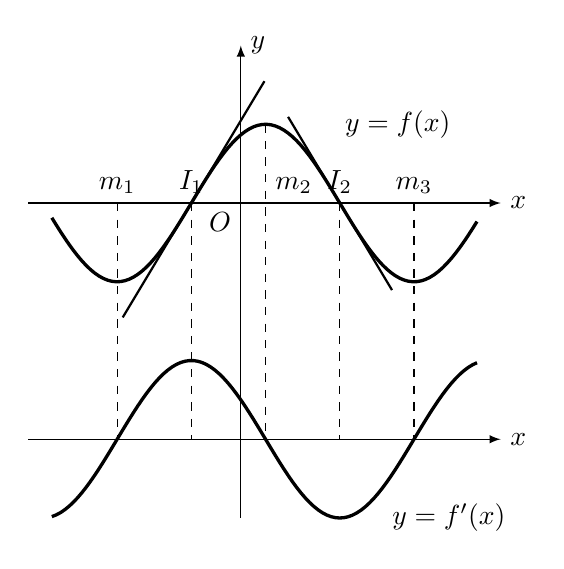
\begin{tikzpicture}[>=latex, xscale=.6]
           \draw[->](-4.5,0)--(5.5,0)node[right]{$x$};
    \draw[->](0,-4)--(0,2)node[right]{$y$};
    \draw[->](-4.5,-3)--(5.5,-3)node[right]{$x$};
    \node at (0,0)[below left]{$O$};
    \draw[domain=-4:5, samples=100, very thick]plot(\x, {sin((\x+pi/3)*180/pi)});
    \draw[domain=-4:5, samples=100, very thick]plot(\x, {cos((\x+pi/3)*180/pi)-3});
    
    \foreach \x/\xtext in {1.5*pi/m_3, -.5*pi/m_1, 0/I_1, pi/I_2}
    {
       \draw[dashed](\x-pi/3, 0)node[above]{$\xtext$}--(\x-pi/3, -3);
    }
    \draw[dashed](.5*pi-pi/3, 1)--(.5*pi-pi/3, -3);
    \node at (.5*pi-pi/3,0)[above right]{$m_2$};
    
    \draw[domain=-2.5:.5, samples=10, thick]plot(\x, {\x+pi/3});
    \draw[domain=1:3.2, samples=10, thick]plot(\x, {-\x+2*pi/3});
    \node at (2,1)[right]{$y=f(x)$};
    \node at (3,-4)[right]{$y=f'(x)$};
        \end{tikzpicture}
        \caption{}
        \end{minipage}
        \end{figure}
    
    在图2.44中,函数$y=f(x)$的图象上的极值点$m_1$, $m_2$和$m_3$, 对应于函数$y=f'(x)$图象上的零点;$y=f(x)$的图象上的拐点对应于$y=f'(x)$的图象上的极值点.
    
    \begin{ex}
    \begin{enumerate}
        \item 讨论下列函数的极值、凸性及拐点,并出函数图象的
        草图;
    \begin{multicols}{2}
    \begin{enumerate}
        \item $f(x)=\frac{1}{1+x^2}$
        \item $y=(x-1)\sqrt[3]{x^2}$
    \end{enumerate}
    \end{multicols}
    \item 如果函数$f(x)$在区间$(a,b)$内有二阶导数,并且向上凸,求证:对于满足条件$a\le x_1<x_2\le b$的任意两点$x_1,x_2$,恒有
    \[f (\lambda x_1+ (1-\lambda) x_2) \ge \lambda f (x_1) + (1-\lambda)f (x_2) ,\quad  0\le\lambda\le 1\]
    如果上面的函数在区间$(a,b)$内向下凸,则应有怎样的结论?
    \item 求证函数
    \begin{enumerate}
        \item $y=\log_ax \; (a>1)$在区间$(0,+\infty)$内是向上凸的;
        \item $f(x)=\sin x$在$[0,\pi]$内是向上凸的;
        \item $\log_a\frac{x_1+x_2}{2}\ge \frac{\log_a x_1+\log_a x_2}{2}\quad (x_1> 0,\; x_2>2)$
        \item $\sin\frac{x_1+x_2}{2}\ge \frac{\sin x_1+\sin x_2}{2}\quad  (0\le x_1,x_2\le \pi)$
    \end{enumerate}
    
    \item 如果函数$f(x)$在$(a,b)$内是向上凸的,求证:对于任意$a\le x_1<x_2<x_3\le b$,$\sum^3_{i=1}\lambda_i=1$,有
    \[f(\lambda_1x_1+\lambda_2x_2+\lambda_3x_3)\ge \lambda_1f(x_1)+\lambda_2f(x_2)+\lambda_3f(x_3)\]
    
    \item  求证对于任意正数$x_1,x_2,x_3$有
    \[\ln\left(\frac{1}{6}x_1+\frac{1}{3}x_2+\frac{1}{2}x_3\right) \ge \ln \left(x_1^{\tfrac{1}{6}}x_2^{\tfrac{1}{3}}x_3^{\tfrac{1}{2}} \right)\]
    \item  若$A,B,C$是任意三角形的三个内角,求证
    \[\sin A+\sin B+\sin C\le \frac{3\sqrt{3}}{2}\]
    又当$A,B,C$为何值时,上面等式成立?
    \item  对于$a>0$, $b>0$, $0<\alpha<1$, $0<\beta<1$,$\alpha+\beta=1$,求证:
    $a^{\alpha}b^{\beta}\le \alpha a+\beta b$成立.
    (提示:利用对数函数是上凸函数)
    \item  $f(x)=a_4x^4+a_3x^3+a_2x^2+a_1x+a_0$为具有正系数
    的非零多项式,若为偶函数,求证$f(x)$在$(-\infty,+\infty)$内向下凸,且仅有一个极值.
    \end{enumerate}
    \end{ex}
    
    \subsection{作函数的图象}
    给出函数$y=f(x)$, 常常希望画出它的图象来,这对于许多问题是有用的,在初中我们所介绍的用列表法来描绘函数的图象,有很大的不精确性和盲目性,由于所取的点是有穷多个,很可能在所要画出的某两点之间的曲线有比较剧烈的变化,如果我们用比较平滑的曲线弧去连结,于是所得
    曲线与实际相差很大.以前各节所介绍的函数性态可以帮助我们断定函数图象的主要特征,因此在取点之前,应先对函数的性态作一番讨论,兹将描绘曲线的一般步骤列出如下:
    
    \begin{enumerate}
    \item 确定函数的定义域;
    \item 确定曲线关于坐标轴的对称性;
    \item 确定曲线与坐标轴的交点(如果不易确定,不必强求);
    \item 确定函数的增减性,极大值与极小值;
    \item 确定函数的凸性与拐点;
    \item 确定曲线的渐近线;
    \item 需要时,还得由曲线方程计算出一些适当的点的坐标;
    \item 把上面所得的结果,按自变量大小顺序列入一个表格内,以观察图形的大概形态,然后描绘成图.
    \end{enumerate}
    
    在用例子说明如何绘图之前,我们需要补充说明如何求曲线的渐近线.
    
    \begin{blk}
        {定义}假设曲线$y=f(x)$不限制在有限平面内,即其上的点$P$可以趋于无穷远,如果曲线的点$P$到直线$\ell:\; ax+ty+c=0$的距离$d$, 当$P$沿曲线趋于无穷远时,
        $d\to 0$,
        那么我们称直线$\ell$为所给曲线的\textbf{渐近线}.
    \end{blk}
    
    \subsubsection{水平渐近线及其求法}
    
    设$\ell_1:\; y=\alpha$是曲线$y=f(x)$的一条渐近线,曲线上的$P(x,f(x))$点到$\ell_1$的距离为
    \[d=|\alpha-f(x)|\]
    因$\ell_1$为渐近线,所以,当$x\to +\infty$或$x\to -\infty$时,应有$d\to 0$, 即
    \[\lim_{x\to+\infty}f(x)=\alpha,\qquad \text{或}\qquad \lim_{x\to -\infty}f(x)=\alpha\]
    反之,若上式成立,则$y=\alpha$必为$y=f(x)$的一条渐近线.
    
    \subsubsection{铅直渐近线及其求法}
    
    设$\ell_2:\; x=\beta$是曲线$y=f(x)$的一条渐近线,又$P(x,f(x))$为曲线上的任意一点,它到$x=\beta$的距离是
    \[d=|\beta-x|\]
    因为$\ell_2$是$y=f(x)$的渐近线,那么
    \[\lim_{x\to\pm\beta} f (x) =\pm\infty\]
    反之,若上式成立,则$\ell_2$为$y=f(x)$的一条渐近线.
    
    例如,对于$y=\frac{1}{x}$, 当$x\to 0$, $y\to \pm\infty$,故$x=0$是$y=\frac{1}{x}$的一条渐近线.
    
    \subsubsection{任意渐近线及其求法}
    
    设直线$\ell_3:\; y=kx+b$是曲线$y=f(x)$的一条渐近线,曲线上任意一点$P(x,f(x))$到直线$\ell_3$的距离是
    \[d=\left|\frac{kx+b-f(x)}{\sqrt{1+k^2}}\right|\]
    因为$\ell_3$是渐近线,所以当$x\to\pm\infty$时,$d\to 0$, 即
    \[kx+b-f (x) \to 0\]
    我们必须用上式求出$k,b$, 才能确定$\ell_3$. 由于当$x\to\pm\infty$时,$\frac{1}{x}\to 0$, 所以
    \begin{align*}
    \lim_{x\to\pm\infty}\left[k+\frac{b}{x}-\frac{f(x)}{x}\right]&=\lim_{x\to\pm\infty}\frac{1}{x}[kx+b-f(x)]\\
    &=\lim_{x\to\pm\infty}\frac{1}{x}\cdot \lim_{x\to\pm\infty}[kx+b-f(x)]=0
    \end{align*}
    由于$b$是常数,故有
    \begin{align}
        k&=\lim_{x\to\pm\infty}\frac{f(x)}{x}\qquad \text{(渐近线方向)}\\
    b&=\lim_{x\to\pm\infty}[f(x)-kx]
    \end{align}
    
    \begin{example}
    求函数$f(x)=-3x^5+5x^3$的极值、拐点,并画出它的图象的草图.
    \end{example}
    
    \begin{solution}
    \begin{enumerate}
    \item 曲线的范围与截距:这函数$f$的定义域与值域都是无限的,它的曲线伸展在整个平面内,与$y$轴的交点是原点,而与$x$轴有三个交点,其零点是$0,\pm\sqrt{\frac{5}{3}}$.
    \item 对称性:因为$f(-x)=-f(x)$, 所以曲线关于原点对称.
    \item 函数的增、减与极值:
    \[f' (x) =-15x^4+15x^2=-15x^2 (x-1) (x+1)\]
    由此知$f(x)$的驻点是$-1, 0, 1$. $f'(x)$的符号变化的情
    况是:
    \begin{itemize}
        \item 当$x<1$时,$f'(x)<0$, 这时$f(x)$递减;
        \item 当$-1<x<1$时, $f'(x)>0$,这时$f(x)$递增;
        \item 当$x>1$时,$f'(x)<0$, 这时$f(x)$递减.
    \end{itemize}
    因此,$x=-1$是极小点,极小值$f(-1)=-2$; $x=1$是极大点,极大值$f(1)=2$.
    \item 函数的凸性与拐点:
    \[f''(x)=-60x^3+30x=-60x\left(x+\frac{\sqrt{2}}{2}\right)\left(x-\frac{\sqrt{2}}{2}\right)\]
    拐点的可能值是$-\frac{\sqrt{2}}{2},0,\frac{\sqrt{2}}{2}$. 又$f''(x)$的符号变化情况是
    \begin{itemize}
        \item 当$x<-\frac{\sqrt{2}}{2}$时,$f''(x)>0$, 此时曲线向下凸;
        \item 当$-\frac{\sqrt{2}}{2}<x<0$时,$f''(x)<0$, 此时曲线向上凸;
        \item 当$0<x<\frac{\sqrt{2}}{2}$时,$f''(x)>0$, 此时曲线向下凸;
        \item 当$x>\frac{\sqrt{2}}{2}$时,$f''(x)<0$, 此时曲线向上凸;
    \end{itemize}
    因此:$x=-\frac{\sqrt{2}}{2},0,\frac{\sqrt{2}}{2}$的点都是拐点.
    
    \item 列表:今将讨论情况列成下表,并作图(如图2.45)
    \end{enumerate}    
    \begin{center}\small
        \begin{tabular}{cccccccccccc}
        \hline
        $x$ & &$-1$&&$-\frac{\sqrt{2}}{2}$&&0&&$\frac{\sqrt{2}}{2}$&&1\\
        \hline
        $f'(x)$& $-$ & 0&$+$&$+$&$+$&0&$+$&$+$&$+$&0&$-$\\
        $f''(x)$&$+$&$+$&$+$&0&$-$&0&$+$&0&$-$&$-$&$-$\\
        $f(x)$&下凸&极小值& $\nearrow$  & $-1.24$&上凸 & 0& 下凸 &1.24& 上凸 & 极大值 & $\searrow$  \\
        & $\searrow $ &$-2$&&&$\nearrow $&&$\nearrow $&&$\nearrow $&2\\
        \hline
        \end{tabular}
        \end{center}
        
    \begin{figure}[htp]
        \centering
    \begin{tikzpicture}[>=latex, xscale=1.5]
    \draw[->](-2.5,0)--(2.5,0)node[right]{$x$};
    \draw[->](0,-3)--(0,3)node[right]{$y$}; 
    \draw[domain=-1.4:1.4, samples=200, very thick]plot(\x, {-3*\x^5+5*\x^3});
    \foreach \x in {-1,-2,1,2}
    {
        \draw(\x,.1)--(\x,0)node[below]{$\x$};
    }
    \node at (0,0)[below right]{$O$};
    \draw[dashed](-.707,-1.24)--(-.707,0)node[above]{$-\tfrac{\sqrt{2}}{2}$};
    \draw[dashed](.707,1.24)--(.707,0)node[below]{$\tfrac{\sqrt{2}}{2}$};
    \node at (1.29,0)[above]{$\sqrt{\tfrac{5}{3}}$};
    
    \end{tikzpicture}
        \caption{}
    \end{figure}
    \end{solution}
    
    
    \begin{example}    
    描绘函数$y=\frac{(x-3)^2}{4(x-1)}$的图象.
    \end{example}
    
    \begin{solution}
        这个函数在$x=1$这点没有定义,并且,当$x\to 1^-$时,$y\to -\infty$; 当$x\to 1^+$时,$y\to +\infty$, 所以$x=1$是曲线的铅直渐近线,曲线在$x=1$这点断开.
        
    求导数,得
    \[y'= \frac{(x+1) (x-3)}{4 (x-1)^2}\]
    
    当$x<-1$时,$y'>0$; 当$-1<x<3$时,$y'>0$. 因此,$x=-1$是极大点;$x=3$是极小点.又极大值$f(-1)=-2$; 极小值$f(3)=0$
    
    求二阶导数,得
    \[y''=\frac{2}{(x-1)^3}\]
    \begin{itemize}
        \item 当$x<1$时,$y''<0$, 曲线向上凸;
        \item 当$x>1$时,$y''>0$, 曲线向下凸,但是曲线在$x=1$这一
        点断开,因此$x=1$不是曲线的拐点.
    \end{itemize}
    
    又因为
    \[y=\frac{(x-3)^2}{4(x-1)}=\frac{1}{4}(x-5)+\frac{1}{x-1}\]
    \[\lim_{x\to \infty}\left[\frac{(x-3)^2}{4(x-1)}-\frac{1}{4}(x-5)\right]=\lim_{x\to\infty}\frac{1}{x-1}=0\]
    这就是说曲线以$y=\frac{1}{4}x-\frac{5}{4}$为渐近线.
    
    综合起来得到下面结果:
    \begin{center}
        \begin{tabular}{cccccccccccc}
        \hline
        $x$ & &$-1$&&0&&1&&3&\\
        \hline
        $y'$& $+$ & 0&$-$&$-$&$-$&$\x$&$-$&0&$+$\\
        $y''$&$-$&$-$&$-$&$-$&$-$&$\x$&$+$&$+$&$+$\\
        $y$&$\nearrow$ &极大值& $\searrow$  & $\searrow$&$\searrow$ & $\x$& $\searrow$ & 极小值 & $\nearrow$  \\
        &  &$-2$&&$-\frac{9}{4}$&$-\infty $&&$+\infty$&0 &\\
        \hline
        \end{tabular}
        \end{center}
    
    画出具体图形如图2.46.
    \begin{figure}[htp]
        \centering
    \begin{tikzpicture}[>=latex]
        \draw[->](-3.5,0)--(6.5,0)node[right]{$x$};
        \draw[->](0,-5)--(0,3)node[right]{$y$}; 
    \draw[domain=-3.5:6.5, samples=10, thick]plot(\x, {0.25*\x -1.25});
    \draw[domain=-3:.7, samples=100, very thick]plot(\x, {(\x-3)^2/(4*(\x-1))});
    \draw[domain=1.3:6, samples=100, very thick]plot(\x, {(\x-3)^2/(4*(\x-1))});
    \node at (0,0)[below left]{$O$};
    \draw[dashed](1,-5)--(1,3);
    \foreach \x in {1,2,3,4}
    {
        \draw(\x,0)node[below]{$\x$}--(\x,.1);
    }
    \foreach \x in {-1,-2}
    {
        \draw(0,\x)node[left]{$\x$}--(.1,\x);
    }
    
    \node at (2,-1)[ right]{$y=\frac{1}{4}x-\frac{5}{4}$};
    \node at (3,1)[ right]{$y=\frac{(x-3)^2}{4(x-1)}$};
    
    \end{tikzpicture} 
        \caption{}
    \end{figure}
    \end{solution}
    
    
    
    \begin{ex}
    \begin{enumerate}
        \item 讨论下列函数的极值、凸性和拐点, 并画出函数图象.
    \begin{multicols}{2}
    \begin{enumerate}
    \item  $y=\frac{6(x-1)}{x^{2}+3}$
    \item  $y=(x-1)^{3}-3(x-1)$
    \item  $y=\frac{x^{4}}{2}-x^{2}$
    \item  $y=1+4 x^{3}-3 x^{4}$
    \item  $y=\sqrt{(x+2)^{2}\left(16-x^{2}\right)}$
    \item  $y=x^{x}\quad (x>0.1)$
    \item  $y=x e^{-x}$
    \end{enumerate}
    \end{multicols}
    
        \item 作下列函数的图象, 并画出渐近线及在拐点处的切线:
        \begin{multicols}{2}
            \begin{enumerate}
                \item $y=x+\frac{1}{x}$
                \item $y=\frac{x^{2}}{1+x^{3}}$
                \item $y=\frac{2 x}{1-x^{2}}$
                \item $y=\frac{x^{3}}{x^{2}-4}$
                \item $y=\frac{(x-5)(x+3)}{(x+2)^{2}}$
    \end{enumerate}
    \end{multicols}
    \end{enumerate}
    \end{ex}
    
    \subsection*{习题2.3}
    \begin{enumerate}
        \item 求函数$f(x)=x^3+ax^2-3bx+c$的图象关于原点对称时,$f(x)$在区间$-2\le x\le 2$上的最小值,其中$b>0$.
        
        \item 函数$f(x)=3x^2-ax^3$在区间$0\le x\le 2$上的最小值
        是$-4$, 求
    \begin{enumerate}
        \item $a$的值
        \item $f(x)$在区间$0\le x\le 2$的最大值$M$
    \end{enumerate}
    \item 设$a,b$为实数,求函数$y=x^3-3ax^2+bx+1$在区间$0\le x\le 1$上单调增加时,点$(a,b)$存在范围,并用图表示出来.
    
    \item 设$f(x)=x^3-5x^2+3x+a$, 在怎样的情况下对于
    $x$的正值,总有$f(x)>0$成立?
    \item 设$a$是常数,对于函数$f(x)=4x^3-3x+a$
    \begin{enumerate}
        \item 求$y=f(x)$的极大值和极小值;
        \item 确定当方程$f(x)=0$有三个不相等的实根时,$a$值的范围.
    \end{enumerate}
    
    \item 讨论函数$y=\frac{x^3}{2 (x+2)}$的极值,凸向,拐点,渐近线,
    并作出它的图象.
    
    \item 求证$\pi<\frac{\sin\pi x}{x(1-x)}\le 4$.
    \item 对于已知半径为$R$的球,求具有最小体积的外切圆锥
    的体积.
    \item 一长方体的对角线长$\sqrt{11}$cm,全面积为$14{\rm cm}^2$, 求它的体积的最大值,并求体积为最大时三边的长.
    \item 一浮标由三部分组成,一个圆筒与两个相等的圆
    锥,其中每一个圆锥的高等于圆筒的高,问当表面积一定时,什么样的形状会有最大的体积.
    \end{enumerate}     
    
